\chapter[Numérique et sciences du réel]{Numérique et sciences du réel}
\label{chap:I}

\lettrine{D}{e nos jours, nombre de personnes possèdent un ordinateur}, que\linebreak ce soit
\parnote{Rappelons toutefois que certains n'ont toujours pas le bénéfice ou la maîtrise, même élémentaire, de tels outils : « fracture numérique » oblige, souvent équivalente de sociale.} 
une station de travail --- isolée ou en réseau, autrement dit et hors accès Internet, souvent synonyme de « à la maison » ou «~au tra\-vail~» ---, un ordinateur portable, une tablette, un \textit{smartphone}, un téléviseur voire une domotique connectés. Tous ces objets ont été créés sur le même modèle et strictement la même architecture conceptuelle.
\parnotes
\vspace*{1pt}

Il est clair que cette présentation générale mérite d'être soutenue par d'autres apports comme, entre autres, les origines du calcul automatisé ou l'évolution de la technologie des transistors. % (cf. \Cref{app:A}).

Pour certains, l'ordinateur reste encore « une boîte noire » mystérieuse --- parfois au sens propre comme figuré --- qui, lorsque tout fonctionne correctement, ne saurait souffrir d'une investigation plus poussée.
Néanmoins, disposer de quelques éléments d'information, tant des points de vue matériels que logiciels, s'avère bénéfique ; ne serait-ce que pour choisir en toute connaissance de cause son équipement, vis-à-vis de commerciaux en conseils, parfois, pour le moins orientés.

\vspace*{-0.5pt}
%----------
\section[Entrailles d'un ordinateur]{Entrailles d'un ordinateur}
\label{sec:I.1}

Sans chercher à entrer dans le détail du fonctionnement d'un ordinateur, il semble cependant utile de pouvoir observer ses différentes composantes et d'en décrire les fonctionnalités qui lui sont associées.

\vspace*{-0.5pt}
\subsection[Démontage et descriptif]{Démontage et descriptif d'un ordinateur}
\label{sub:I.1.1}

\caution[t]<secondcolor>{%
Erwan \textsc{Kerrien} est chercheur en imagerie médicale dans l’équipe \textsc{Inria} \href{https://www.inria.fr/equipes/magrit}{\textsc{Magrit}}. Ses travaux visent à enrichir l'environnement du chirurgien pendant l'opération : techniques de vision par ordinateur, réalité augmentée et simulation guidée par l'image. Chargé de mission en médiation scientifique au centre \textsc{Inria} \textsc{Nancy-Grand Est}, il anime de nombreuses initiatives. Il est un des concepteurs et auteurs du \textsc{Mooc} \textsc{Icn}.}{À propos de l'intervenant}
Dans la perspective de démythifier le sujet, il est d'abord proposé le démontage d'un ordinateur conventionnel 
--- type PC, pour \textit{Personal Computer} en anglais --- afin de montrer les organes qui le compose (cf. \cref{vid:I.1}).
Il est donc question d'explorer les divers éléments génériques d'un ordinateur, depuis les aspects extérieurs connus de tous, jusqu'aux plus intimes, qui en assurent son --- supposé --- bon fonctionnement.	

\subsubsection[Périphériques]{Périphériques}
\label{subsub:I.1.1.1}

Un ordinateur traditionnel répond à un canon préétabli de configuration, qui comprend \textit{a minima} une plus ou moins grosse boîte que l'on appelle \emph{unité centrale}, accompagnée d'un \emph{écran} --- également dénommé \emph{moniteur} en lien avec l'industrie audiovisuelle ou comme anglicisme direct ---, d'un \emph{clavier}, d'une \emph{souris} et, par exemple, d'une \emph{clef} ou d'un \emph{disque dur} de stockage nomade. Tous ces derniers éléments sont dénommés des \emph{\glspl{peripheral}}\sidenote{Périphériques externes : sous-entendu externes à l'unité centrale.} \emph{externes}.

\begin{marginvideo}
	[\label{vid:I.1}Éléments d'un ordinateur.]%
	\movie[width=\marginparwidth,showcontrols]%
		{
\includegraphics[width=\marginparwidth]{./Images/Pictograms/film-strip-dark-electric-blue.png}}%
		{./Videos/Chapter01/vidI-01-umount-computer-HD.mp4}%
	\launchvideo{./Videos/Chapter01/vidI-01-umount-computer-HD.mp4}
\end{marginvideo}

Les \glspl{peripheral} peuvent être disposés \emph{en entrée}, comme le clavier, la souris, une caméra ou un \textit{scanner} et permettre d'alimenter l'ordinateur en instructions et tâches à accomplir. Ils peuvent également être placés \emph{en sortie}, à l'instar d'un moniteur ou d'une imprimante et restituer le travail effectué par la machine. 

D'autres \glspl{peripheral} s'avèrent être à la fois\sidenote{Les écrans « tactiles » des équipements proposés depuis quelques années sur les téléphones mobiles, tablettes et autres ordinateurs portables sont aussi des \glspl{peripheral} d'entrée et de sortie : leur interface --- dite IHM pour Interface Homme-Machine --- permet dans un même temps, de lancer des instructions et d'en récupérer les résultats.} en entrée et en sortie, par exemple un disque dur externe où il est aussi bien possible d'y lire des informations en entrée et d'en inscrire en sortie.

L'ensemble constitué par les \glspl{peripheral} externes est ainsi branché à l'uni\-té centrale\sidenote{Dans le cas de la vidéo \Cref{vid:I.1}, ce type d'unité centrale est communément appelée une « tour ». Il existe désormais sur le marché une large variété de formats d'unité centrale : depuis les mini-PC de bureau  --- et \textit{barebones} à compléter ---, jusqu'aux stations audionumériques des studios d'enregistrement ou bien serveurs de 19 pouces prévus pour être compartimentés « en cascade » --- \textit{rackable} en anglais.} --- généralement à l'arrière ---, sur des prises que l'on appelle des \emph{ports}.
En retournant l'ordinateur, on voit tous les branchements envisageables d'une unité centrale. Ceux-ci sont essentiellement assurés par des ports physiques avec, pour chacun d'entre eux, un type particulier de connectique.

On distingue ainsi des ports \textit{USB}\sidenote{\textit{Universal Serial Bus}, conçu par \textsc{Compaq} et \textsc{MicroSoft} et diffusé à partir de 1996. Les normes ont évoluées des versions 1 à 3 de nos jours, dont la différence essentielle pour l'utilisateur est le débit du transfert des données. Source : \href{https://en.wikipedia.org/wiki/USB}{Wikipedia \faWikipediaW}.} pour notamment les \glspl{peripheral} dits de \emph{stockage de masse} comme les disques durs externes et autres clefs, mais également pour la souris, une caméra, etc. 

Bien que ce format soit maintenant devenu obsolète, on peut aussi trouver sur des machines plus anciennes un ou plusieurs port(s) \textit{PS/2}\sidenote{\textit{Personal System/2}, dont le nom provient des PC \textsc{Ibm} de troisième génération introduits en 1987. Source : \href{https://en.wikipedia.org/wiki/PS/2_port}{Wikipedia \faWikipediaW}.} pour y brancher un clavier ou une souris.

Bien entendu, on dispose également de ports « vidéo » sur lesquels sont connectés les écrans, soit aux formats \textit{VGA} ou  \textit{DVI}\sidenote{\textit{Digital Visual Interface}, développé par la société \textit{Digital Display Working Group} en 1999. Source : \href{https://en.wikipedia.org/wiki/Digital_Visual_Interface}{Wikipedia \faWikipediaW}.} --- là encore en désuétude ---, soit au format \textit{HDMI}\sidenote{Le format HDMI --- \textit{High Definition Multimedia Interface} --- est établi par un large \textit{consortium} de compagnies en 2002. Il est devenu un standard de transfert de données vidéo en haute définition très répandu aujourd'hui. Source : \href{https://en.wikipedia.org/wiki/HDMI}{Wikipedia \faWikipediaW}.} pour les moniteurs les plus récents en haute définition, voire en très haute définition (4K).

On peut enfin avoir des ports FireWire%\sidenote{Normé sous l’appellation IEEE 1394 --- l'IEEE est une association professionnelle de référence en électronique et informatique ---, le FireWire est un standard d'interface de transfert de données à haut débit proposé par \textsc{Apple} au début des années 1990. Comme pour le MIDI en audionumérique, l'USB a surclassé le FireWire en part de marché, bien que les performances techniques soient meilleures à l'origine. Source : \href{https://en.wikipedia.org/wiki/Institute_of_Electrical_and_Electronics_Engineers}{Wikipedia \faWikipediaW}.}
 --- format plutôt abandonné au profit de l'USB, notamment depuis la version 3 ---, mais surtout un port particulier, l'Ethernet%\sidenote{Normé ISO/IEC-802-3, Ethernet est un protocole de réseau à commutation de paquets --- \textit{local area networks} (LAN), \textit{metropolitan area networks} (MAN) et \textit{wide area networks} (WAN) --- qui a vu son réel essor à partir de 1989, conjointement au \textit{World Wide Web}. Source : \href{https://en.wikipedia.org/wiki/Ethernet}{Wikipedia \faWikipediaW}.} (connectique au format RJ45)
, qui montre qu'Internet peut aussi être considéré comme un \gls{peripheral} externe à l'ordinateur de par sa connexion à distance à d'autres équipements. 

\begin{figure}[!hb]
	%\sidecaption{figure}{\label{fig:I.1}Différents ports et connectiques associées d'un ordinateur.}
	\begin{subfigure}[b]{0.35\linewidth}\Centering
		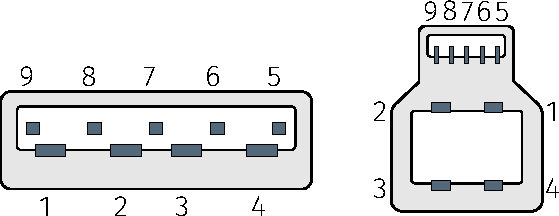
\includegraphics[width=0.9\linewidth]{./Images/Chapter01/figI-01a-usb3.pdf}
		\caption{\label{fig:I.1a}Port USB-3.0, A \emph{versus} B.}
	\end{subfigure}\hfill
	\begin{subfigure}[b]{0.3\linewidth}\Centering
		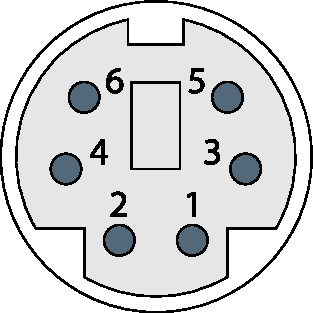
\includegraphics[width=0.40\linewidth]{./Images/Chapter01/figI-01b-ps2.pdf}
		\caption{\label{fig:I.1b}Port PS/2.}
	\end{subfigure}\hfill
	\begin{subfigure}[b]{0.3\linewidth}\Centering
		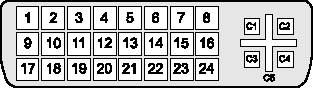
\includegraphics[width=0.70\linewidth]{./Images/Chapter01/figI-01c-dvi.pdf}
		\caption{\label{fig:I.1c}Port DVI.}
	\end{subfigure}\\[8pt]
	\begin{subfigure}[b]{0.35\linewidth}\Centering
		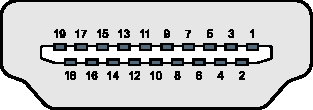
\includegraphics[width=0.65\linewidth]{./Images/Chapter01/figI-01d-hdmi.pdf}
		\caption{\label{fig:I.1d}Port HDMI.}
	\end{subfigure}\hfill
	\begin{subfigure}[b]{0.3\linewidth}\Centering
		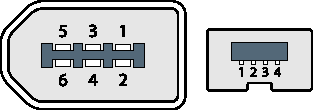
\includegraphics[width=0.75\linewidth]{./Images/Chapter01/figI-01e-firewire.pdf}
		\caption{\label{fig:I.1e}Port FireWire.}
	\end{subfigure}\hfill
	\begin{subfigure}[b]{0.3\linewidth}\Centering
		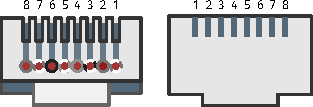
\includegraphics[width=0.8\linewidth]{./Images/Chapter01/figI-01f-rj45-ethernet.pdf}
		\caption{\label{fig:I.1f}Port Ethernet (RJ45).}
	\end{subfigure}
	\caption{\label{fig:I.1}Différents ports et connectiques associées d'un ordinateur.}
\end{figure}

Pour être complet, il faut encore mentionner que la plupart des ordinateurs possèdent des entrées/sorties audio au format mini-jack, respectivement pour un micro et un casque ou système d'enceintes.
De ce point de vue, tout comme pour la vidéo, les composants dédiés au traitement de données audiovisuelles sont désormais très souvent intégrés à l'unité centrale (voir \cref{subsub:I.1.1.2} et \cref{fig:I.2} à suivre).

Bien que les technologies aient considérablement évolué pour intégrer ces fonctionnalités en configuration standard (\gls{motherboard} et processeur), cela répond cependant à des besoins courants d'utilisation. 

Pour des exploitations avancées ou professionnelles --- simulation numérique et prototypage\sidenote{On parle aussi aujourd'hui de « \emph{réalité augmentée} » (voir \cref{subsub:I.3.1.4}).} virtuel, jeux, infographie, musique assistée par ordinateur (MAO), etc. ---, il est nécessaire de compléter un équipement de base par des cartes graphique et/ou audio adéquates, destinées spécifiquement à ces types de données, qui s'avèrent\sidenote{Il s'agit ainsi de déporter la charge de calcul d'opérations connues, donc anticipées, sur des éléments réservés à cet effet, audio comme vidéo.} gourmandes en termes de calculs à effectuer par le processeur.


\subsubsection[Unité centrale]{Unité centrale}
\label{subsub:I.1.1.2}

L'exploration de l'intérieur d'une unité centrale amène à constater beaucoup de choses. Pour commencer par sa relation avec l'environnement extérieur, il faut déjà noter la présence d'un bloc d'alimentation électrique. De cette alimentation sortent un ensemble de fils et de câbles de différentes couleurs qui servent à apporter l'électricité aux multiples composants internes de l'ordinateur.  

En établissant le lien entre les divers ports et les éléments internes d'une unité centrale, on remarque que l'écran est branché sur la \emph{carte graphique}, elle-même enficher sur une grande plaque appelée la \emph{\gls{motherboard}}. Quant à eux, les clavier, souris et disques durs principaux --- dits « maîtres » --- sont directement connectés sur cette même \gls{motherboard}.

Il est enfin à noter que les barrettes de mémoire dites « vives » et les cartes d'extension de tout ordre sont de même intégrées à la \gls{motherboard} \textit{via} leurs ports respectifs : DIMM \textit{versus} PCI.

%\begin{figure}[!hb]
\begin{fullwidth}
  \vspace*{-0.25\baselineskip}
  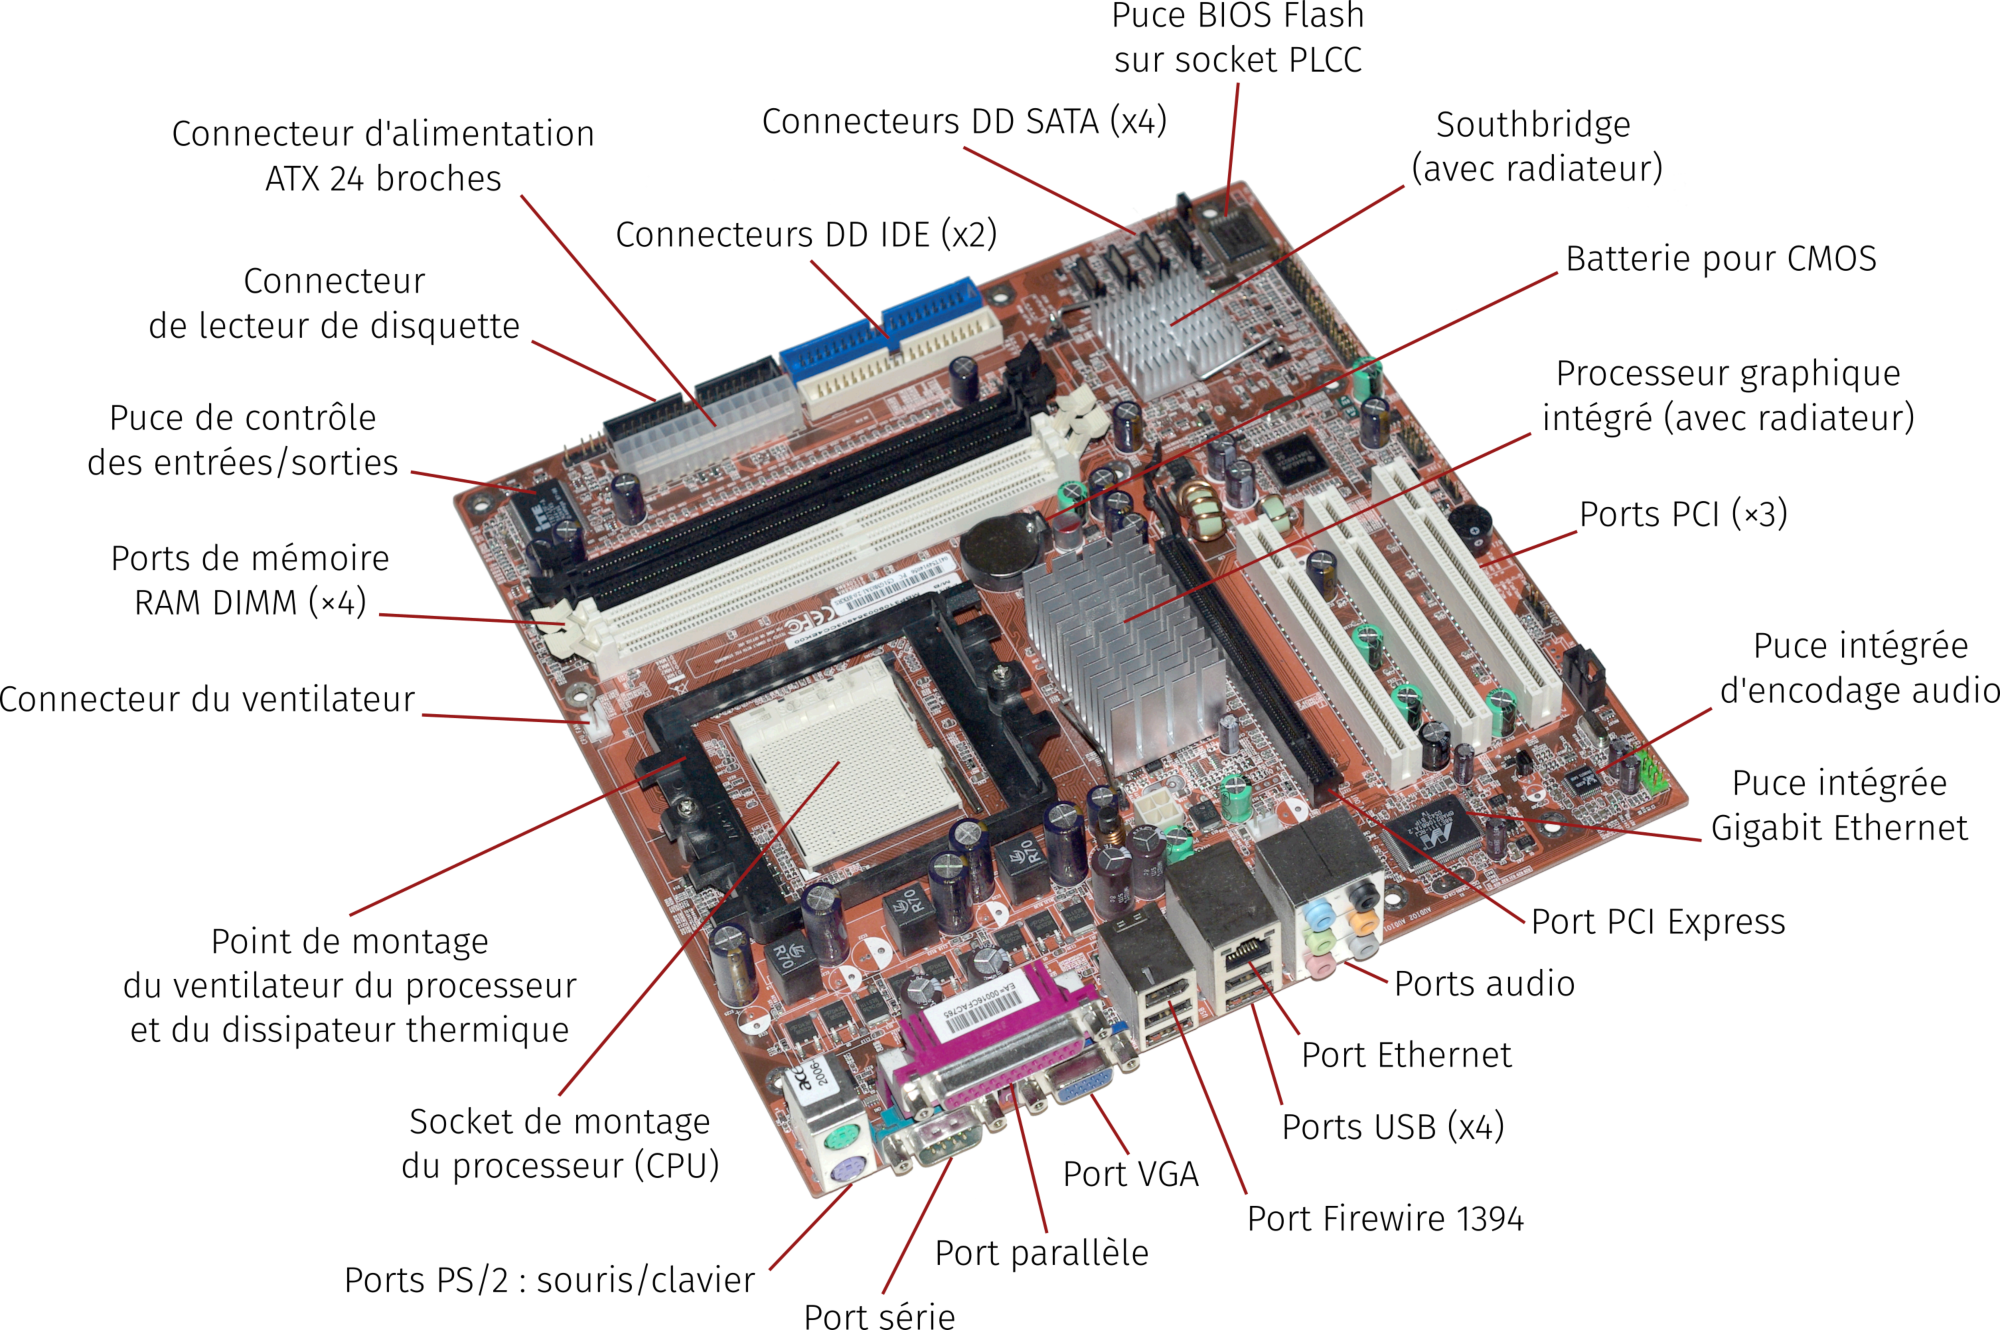
\includegraphics[width=\linewidth]{figI-02-motherboard-comment.png}
  \captionsetup{type=figure}
  \vspace*{-\baselineskip}
  \caption{\label{fig:I.2}Carte mère (assez ancienne, $\approx$ 2005) et ports des périphériques de l'unité centrale.}
\end{fullwidth}
%\end{figure}

Sur certains ordinateurs devenus aujourd'hui obsolètes, mais toujours en service, on observe la présence d'autres composants --- à considérer comme \emph{périphériques internes} ---, à savoir des lecteurs-graveurs de support numérique\sidenote{Les lecteurs/graveurs de type CD/DVD, considérés comme indispensables pour des raisons de puissance de calcul à la fin des années 1990--début 2000, sont désormais définitivement hors-jeu. Si besoin est, on peut s'en procurer à prix modique comme périphérique extérieur en connectique USB. Quant au lecteur de disquette, ils sont avantageusement remplacés par les clefs USB de toutes tailles de stockage.} CD/DVD. En remontant le temps, d'autres matériels antérieurs étaient présents, tels les lecteurs de disquettes...

En effet, la baisse spectaculaire du coût de la mémoire de stockage de masse (disques durs et clefs USB) constatée depuis la fin des années 2000 a modifié en profondeur les comportements et les modes d'usage : qui de sa collection intégrale de photographies de vacances, voire de son système d'exploitation nomade.

Les offres du marché s'affranchissent donc désormais de proposer de telles fonctionnalités pour mettre en avant : puissances de calcul, performances du processeur, capacité et rapidité des périphériques de stockage\sidenote{Mise en exergue des mémoires plus rapides des technologies semi-conducteurs --- SSD pour \textit{Solid-State Drive} --- au regard des mémoires à support magnétique des disques durs conventionnels.} ou qualité de gestion graphique.

Par l'intermédiaire de câbles et de nappes --- bus d'interconnexions en parallèle pour des raisons de performance ---, on constate au global que tous les composants internes d'un ordinateur sont dûment connectés à la \gls{motherboard} \textit{via} des ports spécifiques, mais cette fois internes : dispositifs dédiés tels que cartes d’extension graphique, audio et autres (ports \emph{PCI}\sidenote{\textit{Peripheral Component Interconnect}, un bus initialement dû à \textsc{Intel} dans les années 1990 qui n'a cessé d'évoluer ensuite. On peut citer un de ses dérivés assez largement utilisé, le \textit{PCI-Express} qui a l'ambition de remplacer le PCI, mais également le bus graphique AGP --- \emph{Accelerated Graphics Port}. Source : \href{https://en.wikipedia.org/wiki/Conventional_PCI}{Wikipedia \faWikipediaW}.}), ou bien barrettes de \emph{\gls{RAM}}\sidenote{Il s'agit de mémoire à accès très rapide que le processeur utilise comme tampon pour disposer des données en cours de traitement, en entrée comme en sortie.} --- RAM pour \textit{Ramdom Access Memory} en anglais.

Notamment par effet Joule, les divers composants sollicités d'un ordinateur produisent beaucoup de chaleur. Pour assurer leur bon fonctionnement, des systèmes de refroidissement sont introduits au sein de l'unité centrale.

Plusieurs solutions techniques existent, dont une des plus simples à mettre en œuvre est la ventilation de l'air ambiant, qu'il s'agisse de\linebreak l'unité centrale elle-même, du \emph{\gls{processor}} ou bien d'autres composants comme la carte graphique (voir \cref{fig:I.2}). Les ventilateurs sont source de bruit, ainsi il est parfois fait appel à des conceptions avec des radiateurs en aluminium --- bon diffuseur de chaleur ---, en particulier dans les mini-PC : gain en bruit mais également en encombrement.

\sidegraphic{
\includegraphics[width=.6\linewidth]{usb-logo.png}}
\sidegraphic{
\includegraphics[width=.3\linewidth]{firewire-logo.png}}
\sidegraphic{
\includegraphics[width=.75\linewidth]{hdmi-logo.png}}
À l'observation d'une \gls{motherboard} vierge, débarrassée de tous les éléments venant s'y greffer (cf. \cref{vid:I.1} et \cref{fig:I.2}), on s'aperçoit que le point focal essentiel ou le cœur d'un ordinateur est le \gls{processor}. Tous les composants autour de celui-ci lui sont reliés par des bus optimisés selon les différentes délégations de tâches à accomplir : calculs purs, mémoire vive et zones tampons intermédiaires vis-à-vis des périphériques, fonctions graphiques, etc.

De par son architecture, le \gls{processor} comporte lui-même plusieurs parties complémentaires avec une \emph{unité arithmétique et logique} (UAL) chargée en tant que telle des calculs, mais aussi de zones de mémoires extrêmement rapides dites des « caches » qui permettent de stocker les instructions en cours et les résultats intermédiaires. Là encore, le transfert des données se fait en parallèle pour des raisons de performances accrues.

%\subsubsection*{En synthèse}

\begin{marginfigure}%
	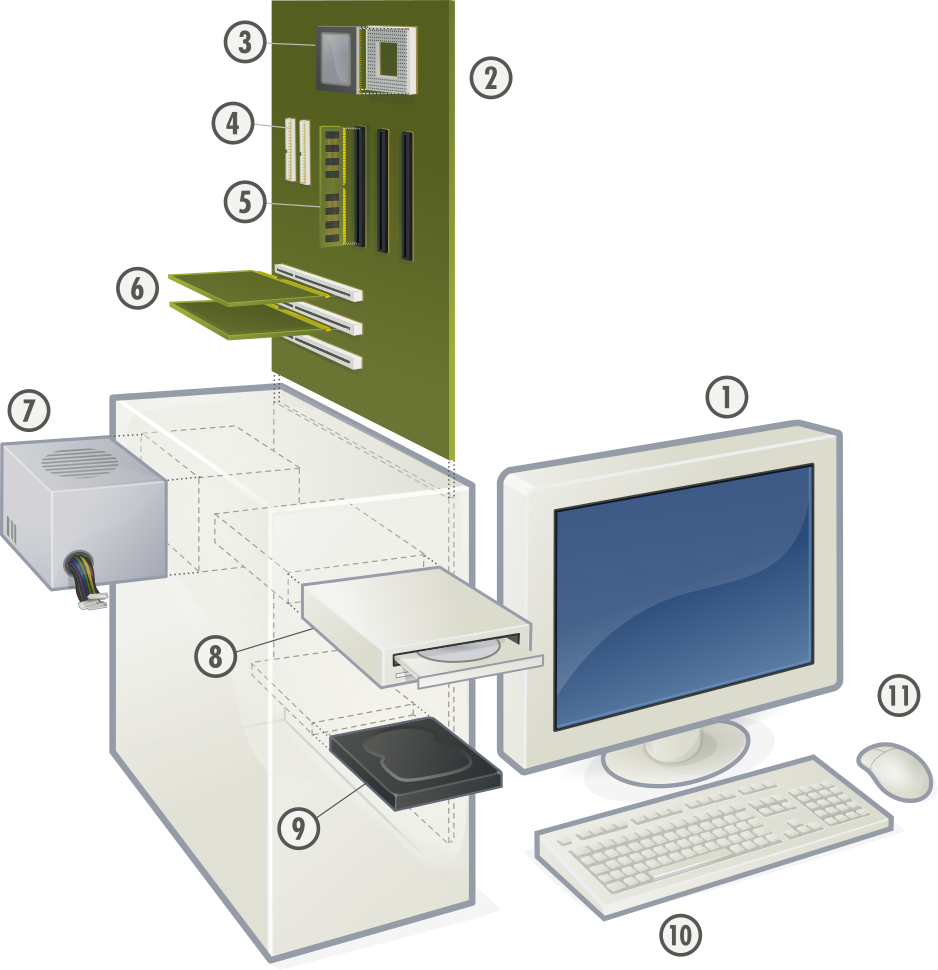
\includegraphics[width=\marginparwidth]{figI-03-exploded-pc-2006.png}
\caption{\label{fig:I.3}Éclaté d'un PC du milieu des années 2000 : 
\Circled{\tiny$1$}
\href{https://fr.wikipedia.org/wiki/\%C3\%89cran_d\%27ordinateur}{écran}, 
\Circled{\tiny$2$}
\href{https://fr.wikipedia.org/wiki/Carte_m\%C3\%A8re}{carte mère}, 
\Circled{\tiny$3$}
\href{https://fr.wikipedia.org/wiki/Processeur}{processeur}, 
\Circled{\tiny$4$}
\href{https://fr.wikipedia.org/wiki/Parallel_ATA}{connecteurs ATA}, 
\Circled{\tiny$5$}
\href{https://fr.wikipedia.org/wiki/M\%C3\%A9moire_vive}{mémoire vive}, 
\Circled{\tiny$6$}
\href{https://fr.wikipedia.org/wiki/Carte_d\%27extension}{carte d'extension}, 
\Circled{\tiny$7$}
\href{https://fr.wikipedia.org/wiki/Alimentation_\%C3\%A9lectrique}{alimentation}, 
\Circled{\tiny$8$}
\href{https://fr.wikipedia.org/wiki/Lecteur_de_CD}{lecteur CD}, 
\Circled{\tiny$9$}
\href{https://fr.wikipedia.org/wiki/Disque_dur}{disque dur}, 
\Circled{\tiny$10$}
\href{https://fr.wikipedia.org/wiki/Clavier_d\%27ordinateur}{clavier}, 
\Circled{\tiny$11$}
\href{https://fr.wikipedia.org/wiki/Souris_\%28informatique\%29}{souris}.}
\end{marginfigure}
Pour effectuer un récapitulatif en opérant un zoom arrière, le \gls{processor} constitue ainsi l'unité fondamentale et centrale de calcul : il est en lien avec tous les autres éléments de l’ordinateur \textit{via} la \gls{motherboard}. Sur cette dernière, toutes les fonctionnalités essentielles sont proposées au moyen de bus spécifiques : accès directs à la \gls{RAM} --- barrettes DIMM ---, au(x) disque(s) dur(s) --- formats IDE ou SATA ---, aux cartes d'extension comme la carte graphique --- connecteur PCI, AGP, voire PCI Express ---, lecteur-graveur de DVD et l'ensemble des ports de périphériques externes par leurs contrôleurs respectifs.

% Contextual glossary (as a subsection)
\printlocalglossary{1}

%\vspace*{-0.25\baselineskip}
\subsection[Montage et fonctionnalités]{Montage et fonctionnalités d'un ordinateur}
\label{sub:I.1.2}

\caution[t]<secondcolor>{%
\href{http://yves.papegay.fr/}{Yves \textsc{Papegay}} est chargé de recherche dans l'équipe \href{https://team.inria.fr/hephaistos/fr/}{\textsc{Héphaïstois}} \textsc{Inria} \textsc{Sophia-Antipolis}. Il s'intéresse aux robots à câbles et à la robotique d'assistance. Il est spécialiste des outils de modélisation et de simulation, de calcul symbolique et d'analyse par intervalles.}{À propos de l'intervenant}
Un ordinateur marque des signes de faiblesse, il est souffreteux, il rame et charger la moindre page Web prend plus de temps que la lire ? Seule solution : le remplacer... Certes, mais l'écran est encore valable, le clavier est comme neuf et la souris toujours aussi véloce.

En étant fortuné, aucune question à se poser, on se rue \textit{illico} chez son fournisseur de prédilection pour acquérir le dernier cri en la matière. En cas contraire où, au-delà des impôts, les factures s'accumulent, où la perspective est d'équiper son association préférée qui, par définition, n'a pas un rond... Existe-t-il une solution ?

\sidegraphic{\href{https://www.raspberrypi.org/}{
\includegraphics[width=.5\linewidth]{raspberry-pi-logo.png}}}
La question ne saurait se poser aussi directement s'il n'était pas envisageable d'y répondre par l'affirmative. En effet, pour environ 50\,€, il est désormais possible depuis quelques années, avec un peu d'huile de coude et en consultant quelques documentations adéquates, de monter par soi-même un ordinateur fonctionnel, n'ayant de plus, rien à envier à une machine de cinq à dix ans révolus. En termes d'application, cela peut être une manière simple et peu onéreuse de maintenir un parc d'ordinateurs dans une salle informatique.

Cette solution remarquable fait appel au projet « \href{https://www.raspberrypi.org/}{\textsc{Raspberry Pi}} ». Initialement motivé par des objectifs pédagogiques et de transmission des savoirs, le succès du projet dépasse ces ambitions premières tant par ses qualités intrinsèques que par la variété des applications possibles : bureautique, domotique, mini-serveur, etc. L'engouement est tel que des revues lui sont partiellement ou entièrement consacrées.

Ayant la préséance, on peut aussi citer le projet « \href{https://www.arduino.cc/}{\textsc{Arduino}} » qui propose au moyen d'une carte électronique modulable, toutes sortes d'expérimentation en électronique numérique. Cependant, toutes choses étant comparables, le \textsc{Raspberry Pi} s'avère un ordinateur complet dans ses fonctionnalités, bousculant un peu le petit monde de l'électronique numérique en créant tout un nouvel écosystème.

\vspace*{-2pt}
\subsubsection[Projet \textsc{Raspberry Pi}]{Projet \textsc{Raspberry Pi}}
\label{subsub:I.1.2.1}

\begin{marginvideo}
	[\label{vid:I.2}Ordinateur Raspberry Pi.]%
	\movie[width=\marginparwidth,showcontrols]%
		{
\includegraphics[width=\marginparwidth]{./Images/Pictograms/film-strip-dark-electric-blue.png}}%
		{./Videos/Chapter01/vidI-02-raspberrypi-HD.mp4}%
	\launchvideo{./Videos/Chapter01/vidI-02-raspberrypi-HD.mp4}
\end{marginvideo}

Le \href{https://fr.wikipedia.org/wiki/Raspberry_Pi}{\textsc{Raspberry Pi}} est une idée un peu folle d'un concepteur anglais de jeux vidéo, \href{https://en.wikipedia.org/wiki/David_Braben}{\textsc{David Braben}}, qui a eu l'ambition de fabriquer un petit ordinateur pour une cinquantaine d'euros (voir\sidenote{\textit{Errata} --- La vidéo contient deux petites erreurs qui sont rectifiées ici :
\begin{sideitemize}
	\item le port vidéo est un port vidéo RCA et non un port S-Vidéo comme annoncé,
 	utile pour se servir d'un « vieux » téléviseur.
	\item l'alimentation des divers modèles 1, 2, 3 (modèle 4 prévu pour 2020) est en principe 5\,V et non pas en 3\,V comme décrit.
\end{sideitemize}
} \cref{vid:I.2}).

En partenariat avec le laboratoire d'informatique de l'\href{https://www.cam.ac.uk/}{Université de Cambridge} et \href{https://www.broadcom.com/}{Broadcom}, une fondation a été créée en 2009 pour promouvoir l'informatique auprès des jeunes publics et plus largement auprès des personnes n'ayant pas les moyens de se procurer un ordinateur, mais pouvant récupérer de vieux matériels : téléviseur, clavier, etc. L'enjeu a ainsi été de concevoir et de faire fabriquer une carte mère et son processeur, disposant de toutes les fonctionnalités d'un ordinateur moderne, comme cœur essentiel d'une machine (cf. \cref{subsub:I.1.1.2}). C'est chose faite depuis février 2012.

Le dimensionnement du \textsc{Raspberry Pi} est délibérément réduit à sa plus simple expression, voulu pour correspondre au format d'une carte bancaire de crédit. Il s'agit d'une carte mère sur laquelle toutes les fonctionnalités d'un ordinateur conventionnel sont présentes, notamment les différents ports de communication, à savoir (en se fondant sur une description du modèle 3\,B) :
\setlength{\columnsep}{-10pt}
\begin{multicols}{2}
\begin{itemize}\jazzitem
\item processeur ARM Cortex A53 Quad-Core 1.2\,GHz ;
\item mémoire vive 1\,Go;
\item un port HDMI, voire un port RCA sur les plus anciennes cartes, pour y brancher un téléviseur ou un écran ;
\item des ports USB\,2 --- quatre sur les cartes récentes --- pour clavier, souris et autres extensions --- selon les cas prévoir toutefois des extensions auto-alimentées pour ne pas perturber le bon fonctionnement du \textsc{Raspberry Pi} ;
\item un port audio au format mini-jack pour un casque ;
\item un port Ethernet et des puces Bluetooth 4.1 et WiFI 802.11n pour les communications ;
\item un connecteur d'alimentation micro-USB.
\end{itemize}
\end{multicols}

%\begin{marginfigure}[\label{fig:I.3}\textsc{Raspberry Pi} modèle 3\,B+.]%
%	\includegraphics[width=\marginparwidth]{./Images/Chapter01/raspberry-pi-3bplus.jpg}
%\end{marginfigure}

% TODO: reprendre raspberry-pi-b-plus-400x282.jpg en plus haute résolution avec les mêmes annotations
% Voir http://gurau-audibert.hd.free.fr/josdblog/2014/10/raspberry-pi-model-b-par-ou-commencer/

\begin{jazzfigure*}
  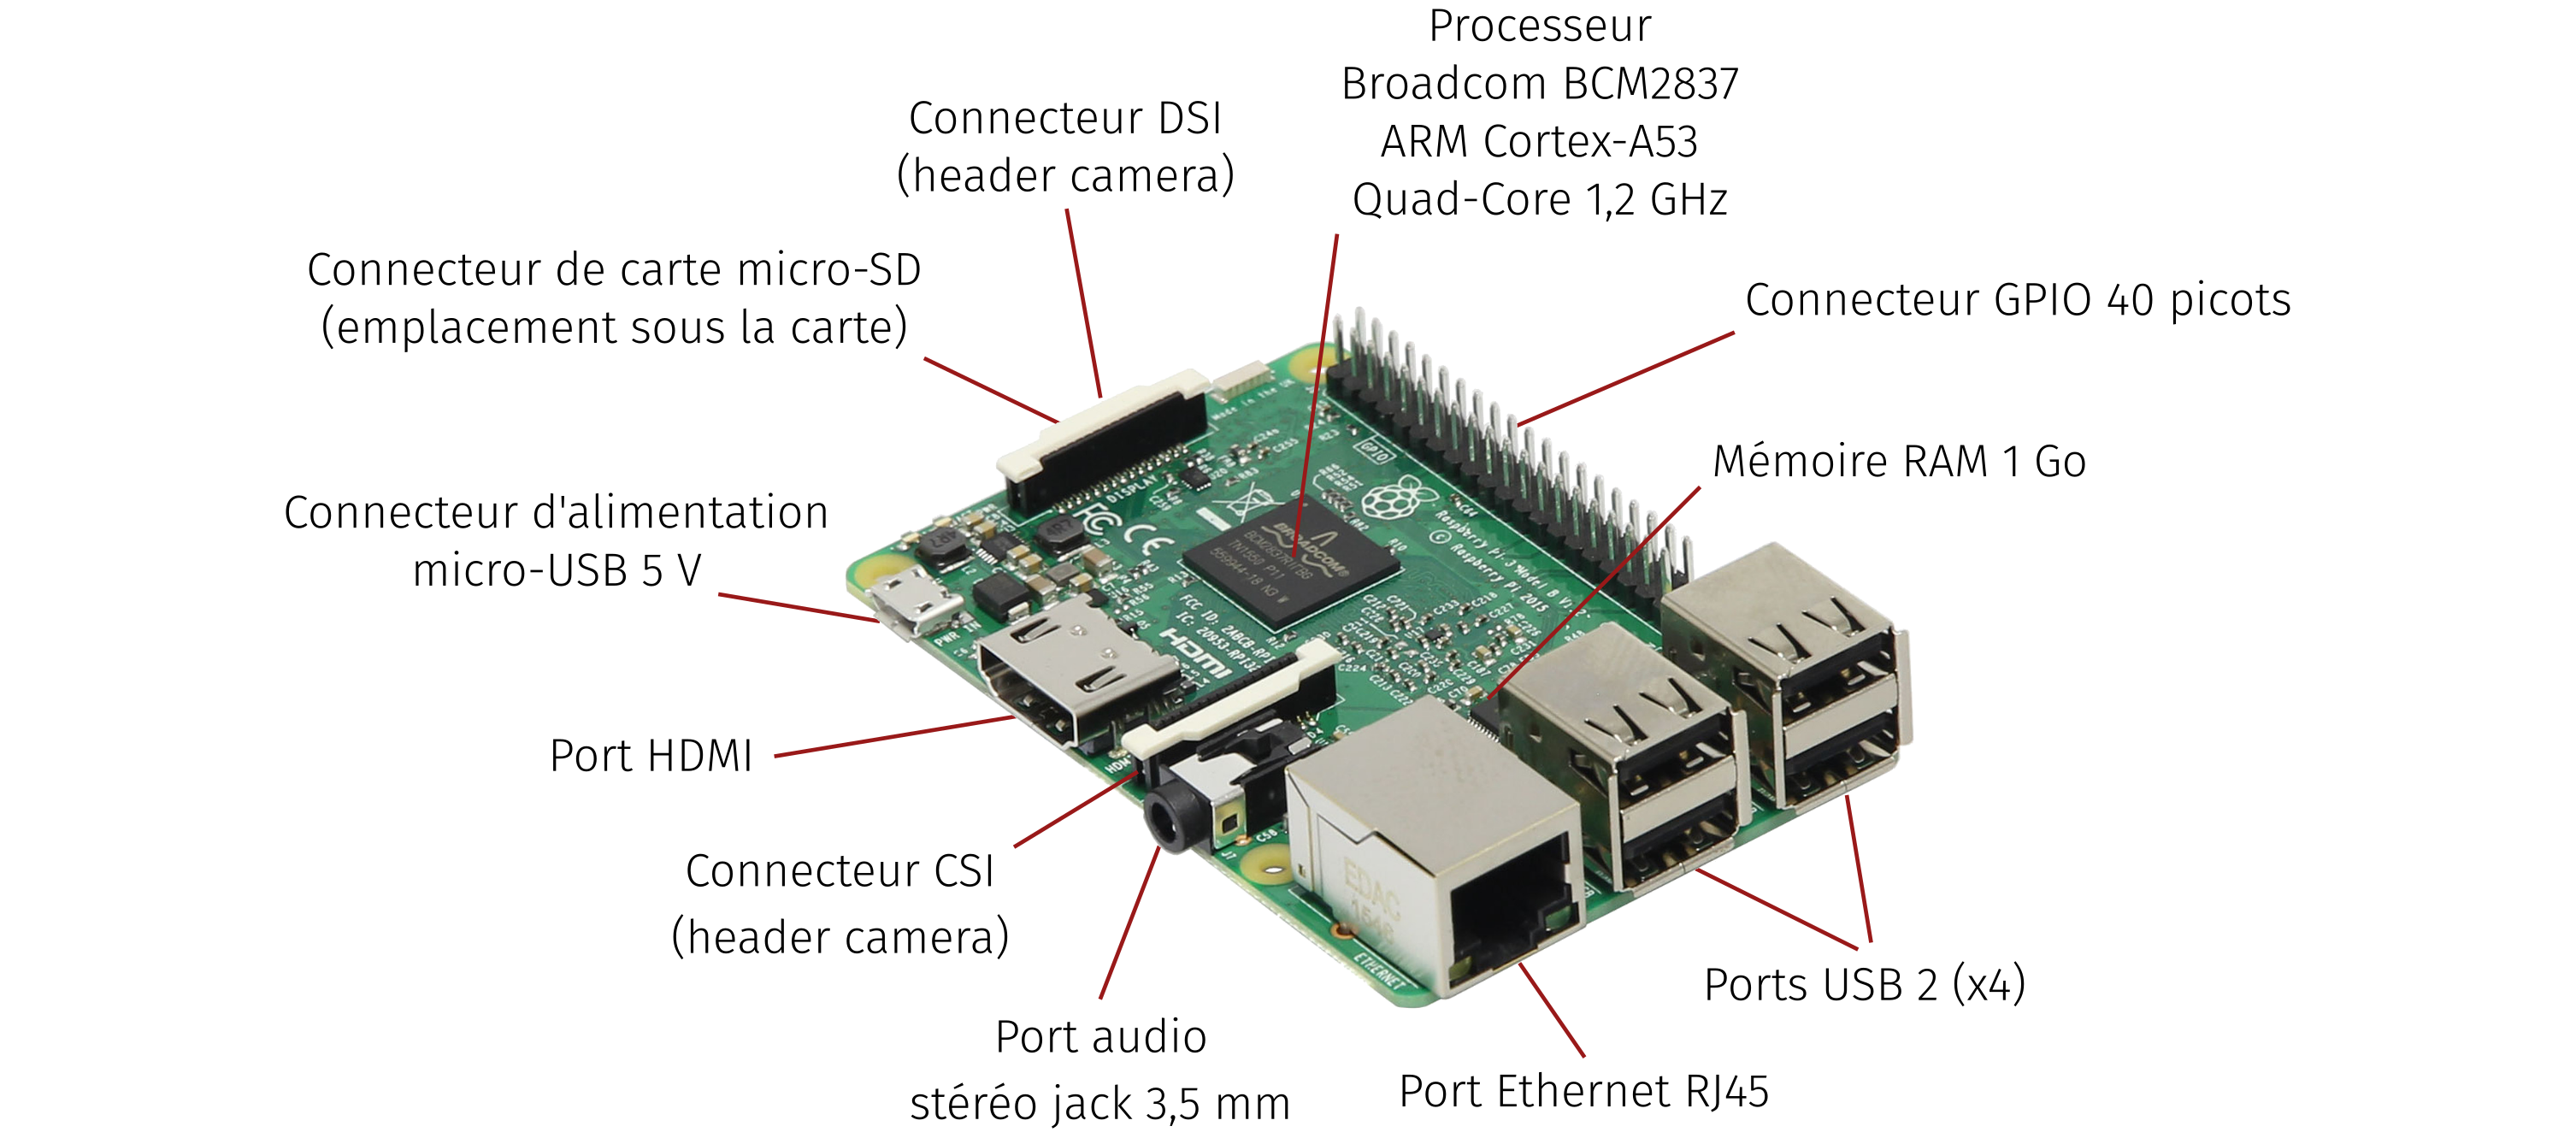
\includegraphics[width=\linewidth]{figI-04-raspberry-pi-3b-comment.png}
  \vspace*{-\baselineskip}
  \caption{\label{fig:I.4}Descriptif du nano-ordinateur \textsc{Raspberry Pi} modèle 3\,B.}
\end{jazzfigure*}

En l'état, ce dispositif ne contient pas tous les composants pour pouvoir être opérationnel. Outre un écran, un clavier et une souris avec leurs câbles associés, il manque en effet une alimentation extérieure et une carte mémoire dite \textit{flash} --- au format dit «~\textit{micro-SD}~» pour faire office régalien de « disque dur » : bien entendu, il est nécessaire de pouvoir enregistrer les données personnelles quelque part.

Enfin, pour les \textsc{Raspberry Pi} les plus anciens, on peut également prévoir un \textit{dongle} USB pour le WiFi ; les plus récents disposent de puces Bluetooth 4.1/4.2 et WiFi n/ac.

Avant de pouvoir faire fonctionner cet ensemble, il faut encore au préalable installer un \gls{OS} (cf. \href{https://fr.wikipedia.org/wiki/Syst\%C3\%A8me_d'exploitation}{\faWikipediaW}) sur la carte micro-SD. Toujours pour des raisons de coût, de dimensionnement et de modularité, le système dûment conseillé est \gls{Linux}. La distribution « historique » du \textsc{Raspberry Pi}, intitulée \href{https://www.raspbian.org/}{\textsc{Raspbian}}, s'est ainsi établie sur une base \gls{GNU/Linux} en version \gls{debianlinux} afin rester dans l'esprit d'ouverture pédagogique du projet initial, incluant en particulier des outils de programmation comme \href{https://scratch.mit.edu/}{\textsc{Scratch}} et \href{https://www.python.org/}{\textsc{Python}}. 

%\tcbsideElement*[t]{
\includegraphics[width=0.5\linewidth]{./Images/Logotype/debian-official-logo-1024px.png}}%
Compte-tenu du succès du projet, de multiples autres possibilités de systèmes d'exploitation libres sont envisageables selon la destination que l'on veut donner à sa machine : serveur réseau ou multimédia, bureautique, domotique, etc. L'essentiel est de choisir un système dont, en particulier l'interface graphique, ne soit pas trop gourmande pour ne pas «~plomber~» le \textsc{Raspberry Pi}. Par exemple, une distribution généraliste comme \href{https://ubuntu-mate.org/}{\textsc{Ubuntu MATE}} a été portée pour cette plateforme.

Passée sous silence jusqu'à présent, une dernière chose est à mentionner avec le \textsc{Raspberry Pi} et qui s'avère non disponible avec un ordinateur conventionnel : le \gls{connector} \gls{GPIO} --- \textit{General Purpose for Input/Output} (cf. \cref{fig:I.4}). Il s'agit d'une interface qui offre la possibilité de communiquer avec d'autres systèmes électroniques et permet au \textsc{Raspberry Pi} d'être utilisé en tant que contrôleur pour, par exemple, piloter un robot, un système de capteurs ou un système embarqué.

% Contextual/local glossary
\printlocalglossary{2}


\subsubsection[Architecture de \textsc{von Neumann}]{Architecture de \textsc{von Neumann}}
\label{subsub:I.1.2.2}

Depuis plus de soixante ans, l’architecture des ordinateurs
\caution[t]<firstcolor>{%
Texte rédigé par Sacha \textsc{Krakoviak} et publié sur \href{https://interstices.info/le-modele-darchitecture-de-von-neumann/}{Interstices} --- revue en ligne de culture scientifique du numérique --- le 18 novembre 2011.}{Note de la rédaction}
est con\-forme à un schéma qui a peu évolué depuis son origine : le modèle dit de « \textsc{von Neumann} ». La naissance de ce modèle, sa diffusion et ses premières mises en œuvre sont un moment-clé de l’histoire de l’informatique et des calculateurs.

Le tableau de ce qu’en 1945 on n’appelait pas encore l’informatique présente un paysage contrasté. D’un côté, la \href{https://interstices.info/le-calcul-une-notion-difficile-a-attraper/}{notion de calcul} effectif a trouvé un cadre rigoureux grâce aux avancées d’une discipline nouvelle née dans les années 1930, la méta-mathématique. Le lambda-calcul du mathématicien \href{http://serge.mehl.free.fr/chrono/church.html}{Alonzo \textsc{Church}} et la \href{https://interstices.info/comment-fonctionne-une-machine-de-turing/}{machine universelle} (abstraite) d’\href{https://interstices.info/turing-a-lassaut-denigma/}{Alan \textsc{Turing}}, schémas dont \textsc{Turing} a montré l’équivalence, sont proposés en 1936 comme base de définition de l’\href{https://interstices.info/quest-ce-quun-algorithme/}{algorithme}, pièce maîtresse du processus calculatoire. D’un autre côté, plusieurs tentatives indépendantes visent à construire des machines électroniques ou électro-mécaniques capables d’exécuter des calculs complexes à grande vitesse. Les précurseurs en sont \href{https://fr.wikipedia.org/wiki/Djon_Atanasov}{John \textsc{Atanasoff}} en 1938 aux États-Unis et \href{https://fr.wikipedia.org/wiki/Konrad_Zuse}{Konrad \textsc{Zuse}} en 1941 en Allemagne.

\sidegraphic[À gauche, John William \textsc{Mauchly} (1907-1980) et à droite, John Adam Presper \textsc{Eckert} (1919-1995).]{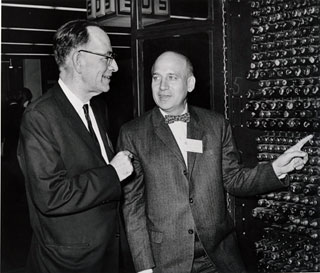
\includegraphics[width=\linewidth]{graphI-01-eckert-mauchly.jpg}}{Computer History Museum}
Ces deux courants, celui des mathématiciens et logiciens d'une part et, celui des ingénieurs d'autre part, sont issus de deux mondes séparés et s’ignorent mutuellement. Les travaux de \textsc{Turing} ont sans doute eu une influence sur la conception en 1943-44 du \href{http://www.histoire-informatique.org/musee/2_3_2.html}{calculateur \textsc{Colossus}} à Bletchley Park en Angleterre, mais il s’agit d’une machine spécialisée dont le seul objectif, qui sera d’ailleurs atteint, est le décryptage du code secret de la machine \textsc{Lorenz}, successeur de l’\href{https://interstices.info/enigma/}{\textsc{Enigma}}, utilisée par l’armée allemande.

La guerre aura d’autres effets : les autorités allemandes ne soutiendront que modestement les travaux pionniers de \textsc{Zuse}, alors que le département américain de la Défense financera un projet ambitieux lancé en 1943 à l’Université de Pennsylvanie par \href{https://fr.wikipedia.org/wiki/John_Eckert}{John Adam Presper \textsc{Eckert}} et \href{https://fr.wikipedia.org/wiki/John_William_Mauchly}{John William \textsc{Mauchly}}. Cet effort aboutira à la construction d’un grand calculateur électronique, l’\textsc{Eniac}, qui ne sera néanmoins pleinement opérationnel qu’en 1946. À cette même époque (1944), l'informaticien \href{https://fr.wikipedia.org/wiki/Howard_Aiken}{Howard \textsc{Aiken}} mène un autre grand projet à Harvard avec la collaboration d’\textsc{Ibm}, mais la technique choisie est fondée sur l'électromécanique. Bien plus fiable que les tubes électroniques, cette voie ne sera toutefois pas poursuivie, mais l’expérience acquise sera exploitée plus tard par \textsc{Ibm} dans la conception de ses premiers ordinateurs.

\sidegraphic[\textsc{Eniac}, à gauche ; panneau de connexion.]{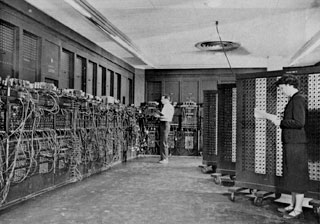
\includegraphics[width=\linewidth]{graphI-02-eniac.jpg}}{U.S. Army}
L’\textsc{Eniac} --- \textit{Electronic Numerical Integrator and Computer} --- fut le premier calculateur entièrement électronique possédant les mêmes capacités qu’une machine de \textsc{Turing}, aux limites physiques près. Il avait des dimensions imposantes : plus de $20$\,m de long, $2$\,m\,$50$ de haut pour une masse de $30$ tonnes. Comportant $18\,000$ tubes électroniques, il consommait 150 kilowatts.

Les données étaient lues sur cartes perforées, mais le programme était représenté sur un support externe, sous la forme d’un panneau de connexion analogue à celui d’un standard téléphonique. Pour programmer une application (initialement, le calcul de tables de tir pour l’artillerie), il fallait faire un plan des connexions nécessaires, puis procéder au câblage physique, un travail long, fastidieux et sujet aux erreurs. La détection et la correction des fautes étaient également laborieuses. Avec la fiabilité réduite des tubes électroniques, ce mode de programmation constituait le grand point faible du projet. Bien conscients de cette faiblesse, ses concepteurs ont commencé dès 1944 à réfléchir à l’étape suivante, avant même la mise en service de l’\textsc{Eniac}.

\sidegraphic[Timbre à l'effigie de \textsc{von Neumann} (1903-1957) émis à titre posthume par son pays natal, la Hongrie.]{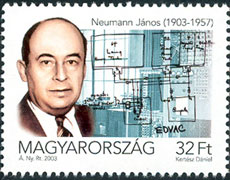
\includegraphics[width=\linewidth]{graphI-03-timbre.jpg}}{Union postale universelle}
En 1944, John \textsc{von Neumann} est introduit dans le projet \textsc{Eniac} par Herman \textsc{Goldstine}, qui assurait la liaison scientifique du projet avec le département de la Défense. \textsc{Von Neumann} était un esprit universel, dont les contributions allaient des mathématiques à la logique, la physique et l’économie. Il avait rencontré Alan \textsc{Turing} et connaissait ses travaux. Il participait alors au projet Manhattan et l’Histoire dit que \textsc{Goldstine} lui parla du projet \textsc{Eniac} lors d’une rencontre fortuite sur un quai de gare. Quoi qu’il en soit, \textsc{von Neumann} accepta un poste de consultant dans ce projet et prit une part active aux travaux menés par \textsc{Eckert} et \textsc{Mauchly} sur la conception de l’\href{https://fr.wikipedia.org/wiki/Electronic_Discrete_Variable_Automatic_Computer}{\textsc{Edvac}} --- \textit{Electronic Discrete Variable Automatic Computer} ---, le successeur de l’\textsc{Eniac}. En juin 1945, une première version, incomplète, d’un rapport sur la conception de l’\textsc{Edvac} fut diffusée par \textsc{Goldstine}, sous la signature du seul \textsc{von Neumann} qui l’avait rédigé comme document de travail. \textsc{Eckert} et \textsc{Mauchly} en furent, à juste titre, profondément choqués ; par ailleurs, ils entrèrent en conflit avec l’Université de Pennsylvanie pour des questions de brevet et ces deux circonstances provoquèrent leur départ du projet en mars 1946 pour fonder leur entreprise, \textsc{Eckert-Mauchly Computer Corporation}. \textsc{Von Neumann} lui-même quitta le projet à la même époque pour Princeton, où il travailla avec Julian \textsc{Bigelow} sur le calculateur de l’\textsc{Ias} --- Institut d’études avancées.

\overparagraph{Architecture novatrice}

%\begin{wrapfigure}{r}{0.5\linewidth}
\begin{marginfigure}
	%\begin{fullwidth}
	%	\includegraphics[width=\linewidth]{figI-03-raspberry-pi-3b-comment.png}
	\begin{tikzpicture}[scale=1.0]
		%\draw [very thin, lightgray] (0,0) grid[step=0.2] (5,6);
		%\draw [very thin, gray] (0,0) grid (5,6);
		\draw[draw=gray, line width=2pt, rounded corners=2pt, fill=firstcolor] 
			(0,5) rectangle 
				node[text=white, font=\scshape\small] {\lightbf{Mémoire}} 
			(5,6);
		\draw[draw=firstcolor, line width=2pt, rounded corners=2pt, fill=white] (-0.05,1.9) rectangle (5.05,4.1);
		\draw[draw=gray, line width=1.6pt, rounded corners=2pt, fill=firstcolor] 
			(0.1,2) rectangle 
				node[text=white, align=center, font=\scshape\small] 
					{\lightbf{Unité}\\ \lightbf{de commande}} 
			(2.35,4);
		\draw[draw=gray, line width=1.6pt, rounded corners=2pt, fill=firstcolor] 
			(2.55,2) rectangle 
				node[text=white, align=center, font=\scshape\small] 
					{\lightbf{Unité}\\ \lightbf{arithmétique}\\ \lightbf{et logique}} 
			(4.9,4);
		\node[draw=gray, rounded corners=2pt, fill=white,
					inner sep=2pt, outer sep=0pt,
					text=secondcolor, font=\scshape\footnotesize]
			(accumulator) at (1.225,2.35) {\lightbf{\footnotesize Accumulateur}};
		\node[draw=gray, rounded corners=1.2pt, fill=white,
					inner sep=2pt, outer sep=0pt,
					text=secondcolor, font=\strut\scshape\footnotesize]
			(input) at (0.5125,0.75) {\lightbf{\footnotesize Entrées}};
		\node[draw=gray, rounded corners=1.2pt, fill=white,
					inner sep=2pt, outer sep=0pt,
					text=secondcolor, font=\strut\scshape\footnotesize]
			(output) at (1.85,0.75) {\lightbf{\footnotesize Sorties}};
		\node[draw=none, rounded corners=0pt, fill=white,
					inner sep=2pt, outer sep=0pt, xshift=1.25cm,
					align=center, text=firstcolor, font=\strut\scshape\small]
			at (2.5,1.25) {\lightbf{Unité centrale}\\ \lightbf{(ou processeur)}};
		\draw[-{Triangle[]}, line width=1pt, draw=secondcolor] (input.north) -- ([xshift=-2pt]accumulator.south);
		\draw[{Triangle[]}-, line width=1pt, draw=secondcolor] (output.north) -- ([xshift=2pt]accumulator.south);
		\draw[{Triangle Cap [reversed]}-{Triangle Cap []}, 
					line width=8pt, draw=secondcolor] (0.725,4) -- (0.725,5);
		\draw[{Triangle Cap [reversed]}-{Triangle Cap []}, 
					line width=8pt, draw=secondcolor] (1.725,5) -- (1.725,4);
		\draw[{Triangle Cap [reversed]}-{Triangle Cap []}, 
					line width=8pt, draw=secondcolor] (3.225,4) -- (3.225,5);
		\draw[{Triangle Cap [reversed]}-{Triangle Cap []}, 
					line width=8pt, draw=secondcolor] (4.225,5) -- (4.225,4);
		%\draw[{Triangle Cap [reversed]}-{Triangle Cap []. Fast Triangle[]}, 
		%			line width=10pt, draw=secondcolor] (0.725,4) -- (0.725,5);
		%\draw[{Triangle Cap [reversed]}-{Triangle Cap []. Fast Triangle[]}, 
		%			line width=10pt, draw=secondcolor] (1.725,5) -- (1.725,4);
		%\draw[{Triangle Cap [reversed]}-{Triangle Cap []. Fast Triangle[]}, 
		%			line width=10pt, draw=secondcolor] (3.225,4) -- (3.225,5);
		%\draw[{Triangle Cap [reversed]}-{Triangle Cap []. Fast Triangle[]}, 
		%			line width=10pt, draw=secondcolor] (4.225,5) -- (4.225,4);
	\end{tikzpicture}
	%\caption{\label{fig:I.4}Modèle originel de \textsc{von Neumann} d’architecture des ordinateurs.}
	\caption{\label{fig:I.5}Modèle originel d’architecture des ordinateurs de \textsc{von Neumann}.}
	%\end{fullwidth}
\end{marginfigure}
%\end{wrapfigure}

Le \textit{First Draft of a Report on \textsc{Edvac}} est un document de cent-une pages qui décrit, d’une part un schéma d’architecture de calculateur, organisé en trois éléments (unité arithmétique, unité de commande et mémoire contenant programme et données) et, d’autre part, des principes de réalisation pour ces éléments, notamment les opérations arithmétiques. Si ce dernier aspect dépend partiellement de la technologie connue à l’époque et a donc nécessairement vieilli, le modèle d’architecture, qui marque une transition profonde avec les pratiques antérieures, reste d’une étonnante actualité. Ce modèle, auquel reste attaché le nom de \textsc{von Neumann}, est exposé par le schéma en \cref{fig:I.5}.

La première innovation est la séparation nette entre l’unité de commande, qui organise le flot de séquencement des instructions et l’unité arithmétique, chargée de l’exécution proprement dite de ces instructions. La seconde innovation, la plus fondamentale, est l’idée du programme enregistré : les instructions, au lieu d’être codées sur un support externe (ruban, cartes, tableau de connexions), sont enregistrées dans la mémoire selon un codage conventionnel. Un compteur ordinal contient l’adresse de l’instruction en cours d’exécution ; il est automatiquement incrémenté après exécution de l’instruction et explicitement modifié par les instructions de branchement.

Un emplacement de mémoire contient indifféremment des instructions et des données. Une conséquence majeure (dont toute la portée n’avait probablement pas été perçue à l’époque) est qu’un programme peut être traité comme une donnée par d’autres programmes. Cette idée, présente en germe dans la machine de \textsc{Turing}, trouve ici sa véritable concrétisation.

\overparagraph{Diffusion et mise en œuvre du modèle}

% Very strange result with vertical alignment! WHY?
\sidegraphic[\textsc{Edvac} installé dans le bâtiment 328 du \emph{Ballistics Research Laboratory}.]{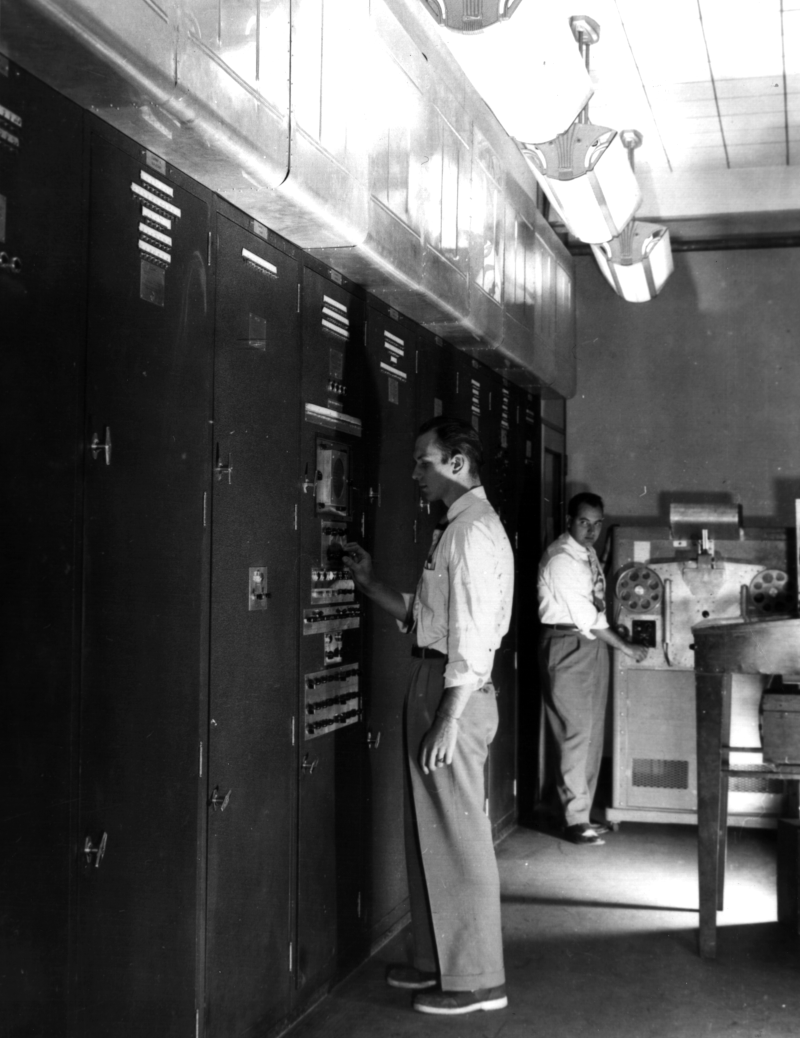
\includegraphics[width=\linewidth]{graphI-04-edvac.png}}{U.S. Army}
Le rapport \textsc{Edvac} circula largement et eut une influence notable sur bon nombre de travaux ultérieurs. En juillet et août 1946, le département de la Défense finança une école d’été pour diffuser les connaissances acquises dans les différents projets de calculateurs. Organisées par la \textit{Moore School} de l’Université de Pennsylvanie, qui abritait le projet \textsc{Eniac}, ces \href{https://en.wikipedia.org/wiki/Moore_School_Lectures}{\textit{Moore School Lectures}} furent un instrument de réflexion sur les concepts et techniques de base des calculateurs et surtout de diffusion des travaux menés dans les projets \textsc{Eniac} et \textsc{Edvac}. \textsc{Eckert} et \textsc{Mauchly}, ainsi que \textsc{Goldstine}, furent les principaux intervenants, mais de nombreux autres conférenciers furent invités, dont Howard \textsc{Aiken} et George \textsc{Stibitz}, qui avaient construit des prototypes de calculateurs. Le seul conférencier non-américain était Douglas \textsc{Hartree}, de l’Université de Manchester. Les auditeurs, au nombre d’une quarantaine, avaient tous été préalablement sélectionnés et invités.

Le projet \textsc{Edvac} lui-même se trouva fortement perturbé par les départs d’\textsc{Eckert} et de \textsc{Mauchly}, que suivirent plusieurs de leurs ingénieurs et ne fut achevé qu’en 1951. Son architecture était fondée sur le modèle présenté dans les \textit{Moore School Lectures}, qui avait évolué par rapport au document originel. 
Entre temps, c’est en Europe que le modèle de \textsc{von Neumann} trouva ses premières réalisations.

\paragraph*{Machines de Manchester}
En 1946, Frederic \textsc{Williams}, alors ingénieur au \textit{Telecommunications Research Establishment} (TRE) en Angleterre --- le siège de l’invention du radar ---, travaillait sur une mémoire utilisant l’écran d’un tube cathodique pour le stockage de bits. Il commença une collaboration avec Thomas \textsc{Kilburn}, de l’Université de Manchester, et obtint un poste dans cette université. L’avantage de la mémoire à tube sur la ligne à retard (technologie dominante à l’époque) était de permettre un accès aléatoire plutôt que séquentiel.

\sidegraphic*[Tube de \textsc{Williams–Kilburn} d'un \textsc{Ibm} 701 au \textit{Computer History Museum}, Mountain View, Californie.]{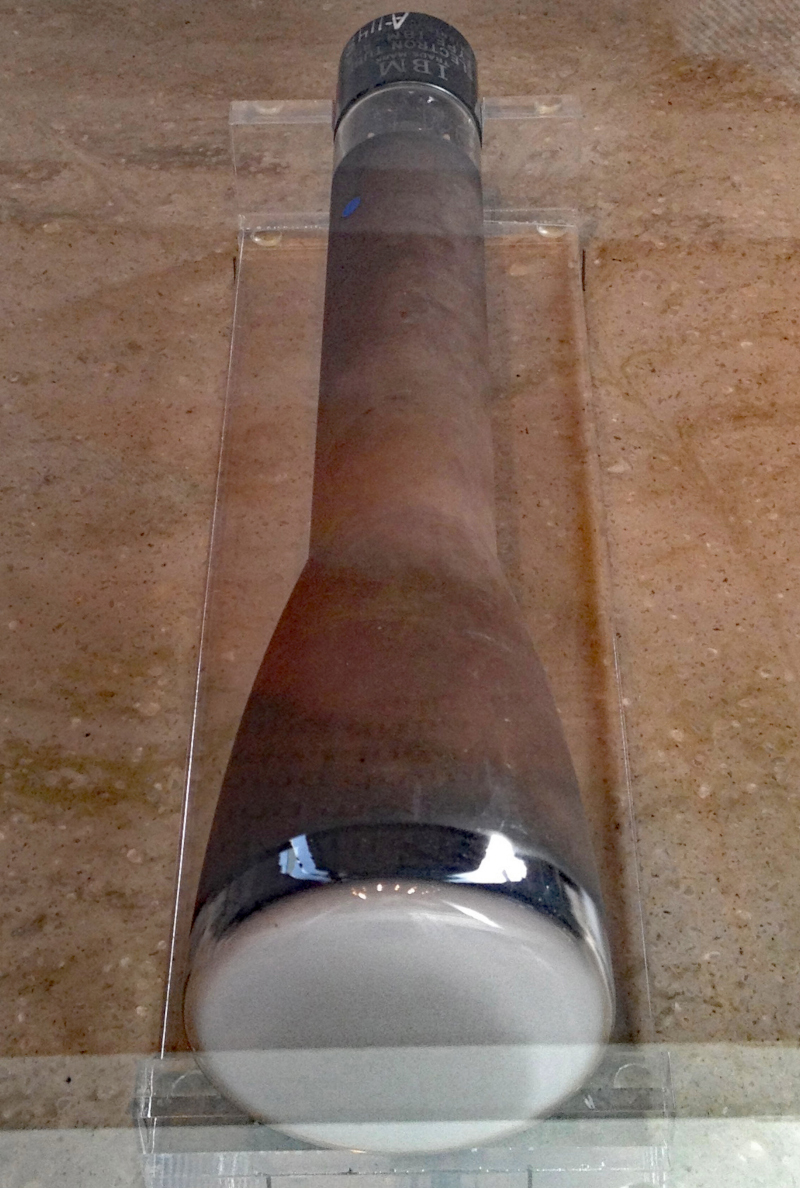
\includegraphics[width=\linewidth]{graphI-05-williams-kilburn-tube.jpg}}{Source : \href{https://en.wikipedia.org/wiki/Williams_tube}{Wikipedia \faWikipediaW}}
En 1947, \textsc{Williams} et \textsc{Kilburn} décidèrent d’expérimenter leur mémoire connue sous le nom de « \href{https://fr.wikipedia.org/wiki/Tube_de_Williams}{tube \textsc{Williams}} » sur un mini-projet de calculateur qu’ils baptisèrent \href{https://www.youtube.com/watch?v=uUa1JRc8Xz0&feature=youtu.be}{\textit{Baby}}. La taille de la mémoire était de $2\,048$ bits. En juin 1948, le premier programme tourna sur le \textit{Baby} ; il avait été inséré bit par bit sur l’écran cathodique.

\textsc{Williams}, \textsc{Kilburn} et leur équipe, que \textsc{Turing} rejoignit en 1948 mais sans y jouer de rôle majeur, construisirent ensuite le calculateur \href{https://fr.wikipedia.org/wiki/Manchester_Mark_I}{Manchester \textit{Mark-1}}. La mémoire à tube était complétée par une mémoire secondaire à tambour magnétique, ce qui était une innovation majeure. \textit{Mark-1} fonctionnait mi-1949. La compagnie \textit{Ferranti} qui était dès cette époque associée au projet, exploita le projet \textit{Mark-1} pour servir de base à son premier produit commercial.
%\vspace*{4pt}

\paragraph*{\textsc{Edsac} de Cambridge}
Maurice \textsc{Wilkes}, qui dirigeait le \textit{Mathematical Laboratory} de l’Université de Cambridge et avait travaillé au TRE sur le radar, perçut très vite les possibilités ouvertes par le rapport \textsc{Edvac}. Il assista aux \textit{Moore School Lectures} en 1946 et lança dès son retour le projet d’un calculateur à programme enregistré appelé \href{https://en.wikipedia.org/wiki/EDSAC}{\textsc{Edsac}} --- \textit{Electronic Delay Storage Automatic Calculator}. Comme l’indique son nom, la mémoire utilisait des \href{https://fr.wikipedia.org/wiki/M\%C3\%A9moire_\%C3\%A0_ligne_de_d\%C3\%A9lai}{lignes à retard}. Le premier programme fonctionna en mai 1949.
On considère généralement l’\textsc{Edsac} comme le premier calculateur à programme enregistré. Bien qu’un programme enregistré ait fonctionné auparavant sur le \textit{Manchester Baby}, ce dernier n’était pas un calculateur complet mais essentiellement un outil de validation du tube \textsc{Williams}. Quoi qu’il en soit, Manchester et Cambridge ont été des pionniers en la matière.

\sidegraphic[Maurice \textsc{Wilkes} (1913-2010) face à la mémoire de l’\textsc{Edsac}.]{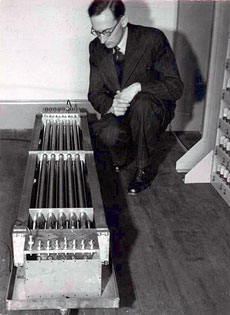
\includegraphics[width=\linewidth]{graphI-06-wilkes-edsac.jpg}}{Computer Laboratory, University of Cambridge}
L’\textsc{Edsac} comportait $1\,024$ emplacements de mémoire de $18$ bits et représentait les nombres entiers en \href{https://fr.wikipedia.org/wiki/Compl\%C3\%A9ment_\%C3\%A0_deux}{complément à $2$} --- mode de codage le plus courant à l’heure actuelle. Il n’avait pas à proprement parler de système d’exploitation, mais des « ordres initiaux » câblés, qui remplissaient les fonctions d’un chargeur. Une invention déterminante, due à David \textsc{Wheeler}, fut celle des \href{https://fr.wikipedia.org/wiki/Sous-programme}{sous-programmes}. La bibliothèque de sous-programmes --- une centaine --- était stockée sous forme de bandes de ruban perforé. Pour utiliser un sous-programme, on devait le copier physiquement sur le ruban contenant le programme utilisateur. La fonction d’éditeur de liens était donc réalisée à la main par des moyens mécaniques !

Le guide du programmeur\sidenote{M.~V.~\textsc{Wilkes}, D.~J.~\textsc{Wheeler}, S.~\textsc{Gill}, \textit{The preparation of programs for an electronic digital computer}. Addison-Wesley, 1951.} de l’\textsc{Edsac}, qui décrit notamment l’utilisation des sous-programmes, fut alors le premier ouvrage consacré à la programmation. \textsc{Wilkes} inventa aussi en 1951 la micro-programmation, exploitée seulement dix ans plus tard dans la famille des \href{https://en.wikipedia.org/wiki/IBM_System/360}{\textsc{Ibm/360}}.
%\vspace*{4pt}

\paragraph*{Autres projets}
Au début de 1946, Alan \textsc{Turing} lança au \textit{National Physical Laboratory} (NPL) un projet de calculateur à programme enregistré, l’\textit{Automatic Computing Engine} (ACE). \textsc{Turing} ne pouvait pas faire état de l’expérience du \textsc{Colossus}, protégé par le secret militaire. Cette circonstance, ajoutée à des problèmes d’organisation, retarda l’avancement des travaux et \textsc{Turing} quitta le NPL en 1948 pour Manchester. Le projet n’aboutit qu’en 1950.

Le projet IAS fut lancé à Princeton par \textsc{von Neumann} en 1946. Son principal ingénieur était \textsc{Bigelow}. La machine commença à fonctionner à l’été 1951 et devint opérationnelle un an plus tard. Elle possédait 1\,024 emplacements de mémoire de 40 bits, réalisés par des tubes \textsc{Williams}.

\overparagraph{Premières machines commerciales}

La compagnie \textsc{Ferranti}, qui fabriquait des équipements électriques et électroniques, collaborait depuis 1948 avec l’équipe de Manchester. Son premier produit, le \textsc{Ferranti} Mark-1 était directement inspiré du Manchester Mark-1. Sorti en février 1951, ce fut le premier calculateur diffusé commercialement.

\sidegraphic*[Console de l'\textsc{Univac-I}.]{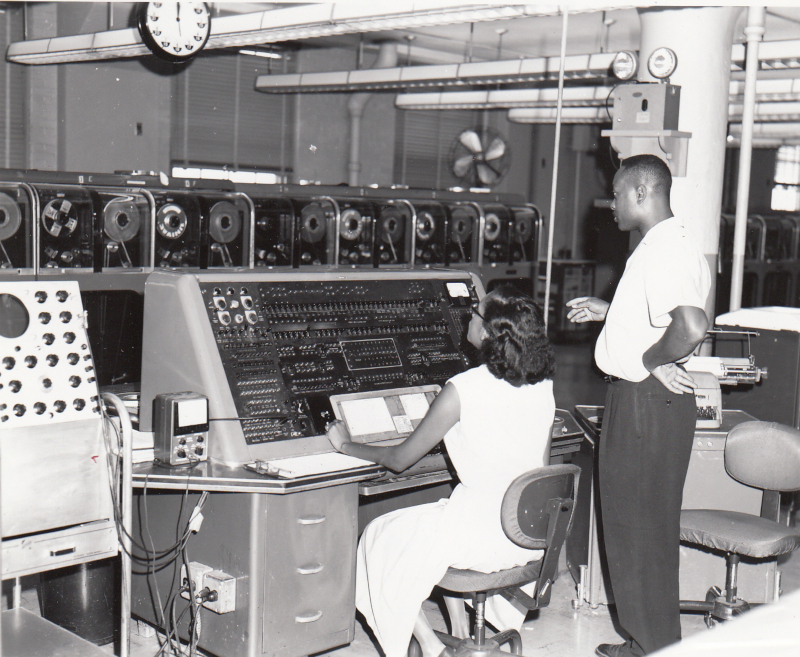
\includegraphics[width=\linewidth]{graphI-07-univacI-console.jpg}}{Source : \href{https://en.wikipedia.org/wiki/UNIVAC_I}{Wikipedia \faWikipediaW}}
La compagnie \textsc{Eckert-Mauchly} (EMCC --- Eckert-Mauchly Computer Corporation) a continué le travail commencé lors de la conception de l’\textsc{Edvac}, en préparant un \textsc{Edvac-2}, qui fut rebaptisé ensuite \textsc{Univac}. En attendant l’aboutissement de ce projet de grande ampleur, EMCC construisit le calculateur \textsc{Binac} pour la société \textsc{Northrop} en 1949. Con\-frontée à des difficultés financières, EMCC fut rachetée en 1950 par \textsc{Remington Rand} (fabricant d’armes et de machines à écrire) et devint la division \textsc{Univac} de \textsc{Remington Rand}. Le premier \textsc{Univac-1} fut livré en juin 1951. La société \textsc{Univac} resta longtemps une référence pour les ordinateurs de grande puissance.

Comparativement, le premier ordinateur d’\textsc{Ibm}, le 701 (qui utilisait les tubes \textsc{Williams}), fut annoncé mi-1952.

\overparagraph{Qu’en est-il aujourd’hui ?}

Plus de soixante ans après son invention, le modèle d’architecture de \textsc{von Neumann} régit toujours l’architecture des ordinateurs. Par rapport au schéma initial, on peut noter deux évolutions essentielles :
\begin{itemize}
\item les entrées-sorties, initialement commandées par l’unité centra\-le, sont depuis le début des années 1960 sous le contrôle de processeurs autonomes (canaux d’entrée-sortie et mécanismes assimilés). Associée à la multiprogrammation (partage de la mémoire entre plusieurs programmes), cette organisation a notamment permis le développement des systèmes en temps partagé ;
\item les ordinateurs disposent maintenant de processeurs multiples, qu’il s’agisse d’unités séparées ou de « cœurs » multiples à l’intérieur d’une même puce. Cette organisation permet d’atteindre une puissance de calcul élevée sans accroître la vitesse des processeurs individuels, limitée par les capacités d’évacuation de la chaleur dans des circuits de plus en plus denses.
\end{itemize}

Ces deux évolutions ont pour conséquence de mettre la mémoire, plutôt que l’unité centrale, au centre de l’ordinateur et d’augmenter ainsi le degré de parallélisme dans le traitement et la circulation de l’information. En revanche, elles ne remettent pas en cause les principes de base que sont la séparation entre traitement et commande, ainsi que la notion de programme enregistré.

\begin{figure}[!hb]
	\vspace*{2pt}
	\begin{tikzpicture}[scale=1.1]
		%\draw [very thin, lightgray] (0,0) grid[step=0.2] (10,3);
		%\draw [very thin, gray] (0,0) grid (10,3);
		\node[draw=gray, rounded corners=1.2pt, fill=white,
					inner sep=2pt, outer sep=0pt,
					text=secondcolor, font=\strut\scshape\footnotesize]
			(input) at (0.75,2.0) {\lightbf{\footnotesize Entrées}};
		\node[shape=rectangle, draw=gray, rounded corners=1.2pt, fill=gray!50,
					inner sep=2pt, outer sep=0pt, minimum width=0.5cm, minimum height=0.5cm] (inputbis) at (2.5,2.0) {};
		\node[draw=gray, rounded corners=1.2pt, fill=white,
					inner sep=2pt, outer sep=0pt,
					text=secondcolor, font=\strut\scshape\footnotesize]
			(output) at (0.75,1.0) {\lightbf{\footnotesize Sorties}};
		\node[shape=rectangle, draw=gray, rounded corners=1.2pt, fill=gray!50,
					inner sep=2pt, outer sep=0pt, minimum width=0.5cm, minimum height=0.5cm] (outputbis) at (2.5,1.0) {};
		\draw[draw=gray, line width=2pt, rounded corners=2pt, fill=firstcolor] 
			(4.0,0) rectangle 
				node[text=white, font=\scshape\small] {\lightbf{Mémoire}} 
			(6.0,3);
		\draw[draw=firstcolor, line width=2pt, rounded corners=2pt, fill=white] (7.8,1.7) rectangle (9.2,3.0);
		\draw[draw=gray, line width=1.6pt, rounded corners=2pt, fill=firstcolor] 
			(7.9,2.4) rectangle node[text=white, align=center, font=\scshape\small] {\lightbf{UC}} (9.1,2.9);
		\draw[draw=gray, line width=1.6pt, rounded corners=2pt, fill=firstcolor] 
			(7.9,1.8) rectangle node[text=white, align=center, font=\scshape\small] {\lightbf{UAL}} (9.1,2.3);
		\draw[draw=firstcolor, line width=2pt, rounded corners=2pt, fill=white] (7.8,0.0) rectangle (9.2,1.3);
		\draw[draw=gray, line width=1.6pt, rounded corners=2pt, fill=firstcolor] 
			(7.9,0.7) rectangle node[text=white, align=center, font=\scshape\small] {\lightbf{UC}} (9.1,1.2);
		\draw[draw=gray, line width=1.6pt, rounded corners=2pt, fill=firstcolor] 
			(7.9,0.1) rectangle node[text=white, align=center, font=\scshape\small] {\lightbf{UAL}} (9.1,0.6);
		\draw[line width=1pt, draw=secondcolor] (input.east) -- (inputbis.west);
		\draw[{Triangle[]}-, line width=1pt, draw=secondcolor] (output.east) -- (outputbis.west);
		\draw[-{Triangle[]}, line width=1pt, draw=secondcolor] (inputbis.east) -- (4.0,2.0);
		\draw[line width=1pt, draw=secondcolor] (4.0,1.0) -- (outputbis.east);
		\draw[{Triangle Cap []}-{Triangle Cap [reversed]}, line width=6pt, draw=secondcolor] (6.0,2.6) -- (7.8,2.6);
		\draw[{Triangle Cap [reversed]}-{Triangle Cap []}, line width=6pt, draw=secondcolor] (6.0,2.1) -- (7.8,2.1);
		\draw[{Triangle Cap []}-{Triangle Cap [reversed]}, line width=6pt, draw=secondcolor] (6.0,0.9) -- (7.8,0.9);
		\draw[{Triangle Cap [reversed]}-{Triangle Cap []}, line width=6pt, draw=secondcolor] (6.0,0.4) -- (7.8,0.4);
		\node[rotate=-90, draw=gray, line width=1pt, 
					inner sep=2pt, outer sep=0pt,
					text=secondcolor, font=\strut\scshape\footnotesize] (processors) 
			at (9.75,1.5) {\lightbf{Processeurs}};
		\node[text=gray, inner sep=0pt, outer sep=0pt] 
			at (8.5,1.4) {\huge\textbullet \textbullet \textbullet};
	\end{tikzpicture}
	\vspace*{2pt}
	\caption{\label{fig:I.6}Modèle actuel de \textsc{von Neumann}.}
\end{figure}

L’accès des processeurs à la mémoire se fait à travers un bus (non représenté sur la \cref{fig:I.6}), voie d’échange assurant un transfert rapide de l’information. Mais au cours du temps, pour des raisons technologiques, le débit du bus a crû moins vite que le débit d’accès à la mémoire et surtout que la vitesse des processeurs. D’où un phénomène d’attente --- le « goulot de \textsc{von Neumann} » --- qui réduit les performances. Des palliatifs sont associés à l’usage généralisé de \href{https://interstices.info/et-plus-vite-si-affinites/}{caches} à plusieurs niveaux (mémoire d’accès rapide, voisine du processeur qui retiennent les données courantes) et au développement de machines à mémoire distribuée, mais se posent alors des problèmes de cohérence pour les données en copies multiples.

Quel modèle de machine après \textsc{von Neumann} ? La question, posée depuis longtemps, n’a pas de réponse claire aujourd’hui (voir le document « \href{https://interstices.info/calculer-differemment/}{Calculer différemment} », Interstices, 2011).

%\sidegraphic*{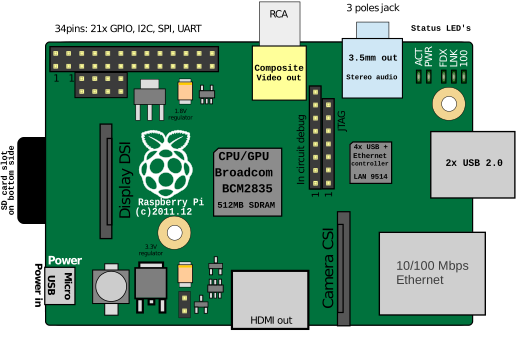
\includegraphics[width=\linewidth]{raspberry-pi-scheme.png}}
\begin{gofurther}[after skip=2pt]
\textsc{\lightbf{Autour du Raspberry Pi}}
\begin{itemize}\jazzitem
\item Manuel d’utilisation du \textsc{Raspberry Pi} --- format PDF, \href{./Documents/Chapter01/docI-01-raspberry-pi-adventures.pdf}{\textit{Adventures in Rasperry Pi \& Rasperry Pi User Guide}} ---, à destination des adolescents pour découvrir les possibilités du \textsc{Raspberry Pi} ;
\item \href{http://binaire.blog.lemonde.fr/2015/12/28/raspberry-pi-la-petite-histoire-dune-grande-idee/}{\textit{\textsc{Raspberry Pi} : la petite histoire d’une grande idée}}, Binaire, 28 décembre 2015 ;
\item \href{https://www.france24.com/fr/20161225-comment-installer-raspberry-pi-nano-ordinateur-a-moins-50-euros}{\textit{Comment installer un \textsc{Raspberry Pi}, ce nano-ordinateur à moins de 50 euros}}, avec une présentation vidéo de \textsc{Raspberry Pi} par Alan \textsc{McCullagh}, décembre 2016.
\end{itemize}

\smallskip
\textsc{\lightbf{Architectures avancées pour plus de puissance de calcul}}
\begin{itemize}\jazzitem
\item \textit{Le futur de l'ordinateur ? \href{https://interstices.info/vers-lordinateur-quantique-un-defi-scientifique-majeur-pour-les-prochaines-decennies/}{L'ordinateur quantique}}, Philippe Jorrand, Interstices, 2005 ;
\item \href{http://binaire.blog.lemonde.fr/2016/04/08/sil-vous-plait-dessine-moi-un-superordinateur/}{\textit{Architecture et performance : les super-ordinateurs}}, Charlotte Truchet, binaire, 08 avril 2016 ;
\item \href{https://www.canal-u.tv/video/inria/les_machines_d_aujourd_hui_et_de_demain.6490}{\textit{Les machines d'aujourd'hui et de demain}}, Albert Cohen,  CanalU, collection Inria Science Info Lycée Profs ; 86\,mn. montrant les liens entre science informatique et architecture des ordinateurs ;
\item \href{https://www.youtube.com/watch?v=U9T0fjFyVow}{\textit{Microcontrôleur : Comment ça marche ?}} --- SILIS Electronique, 25 février 2016 : 5\,mn 34\,s ---
Tout objet numérique n'a pas un processeur, une carte graphique, un disque dur... Alors pourquoi dit-on que tous ces objets fonctionnent sur le même schéma ? Parce qu'ils intègrent un \emph{microcontrôleur} qui suit la même architecture matérielle. Cette \href{https://www.youtube.com/watch?v=U9T0fjFyVow}{vidéo} en donne une introduction claire.
\end{itemize}
\end{gofurther}


%----------
\section[Système d’exploitation]{Système d’exploitation}
\label{sec:I.2}

\caution[t]<secondcolor>{%
Damien \textsc{Saucez} est chercheur au sein de l'équipe  \textsc{Inria}-\href{https://www.inria.fr/equipes/diana}{\textsc{Diana}}. Il consacre ses travaux aux réseaux information-centrés (\href{https://en.wikipedia.org/wiki/Information-centric_networking}{\textit{Information-centric networking}}) --- par exemple, les problèmes de routage et de contrôle de la congestion ---, aux réseaux définis par logiciel (\href{https://fr.wikipedia.org/wiki/Software-defined_networking}{\textit{Software Defined Networking}} --- en particulier, les questions de résilience et de robustesse --- et aux expérimentations à large échelle. Il est un contributeur actif de l'\href{https://en.wikipedia.org/wiki/Internet_Engineering_Task_Force}{\textsc{Ietf}} et de l'\href{https://en.wikipedia.org/wiki/Internet_Research_Task_Force}{\textsc{Irtf}}.}{À propos de l'intervenant}
En usage courant d'un ordinateur --- quel qu'il soit ---, lors du lancement d'une application de lecture de vidéo, les images apparaissent à l'écran et du son est émis par les haut-parleurs. Dans le même temps, le gestionnaire de courrier électronique peut se manifester en prévenant de l'arrivée d'un nouveau message, auquel il est possible de répondre en saisissant du texte au clavier sans avoir à quitter le lecteur vidéo --- et, en toute convenance pratique, sans obliger à reprendre la lecture depuis le début alors que le dénouement est proche !

Comment une application peut-elle ainsi interagir avec les périphériques matériels ? Comment deux applications peuvent-elles tourner en même temps sur un seul processeur ? Tout ceci est possible grâce au \emph{système d'exploitation}, une couche logicielle intermédiaire entre la couche applicative et celle du matériel, dont les principes de fonctionnement sont à découvrir en trois concepts clefs.

\begin{marginvideo}
	[\label{vid:I.3}Système d'exploitation.]%
	\movie[width=\marginparwidth,showcontrols]%
		{
\includegraphics[width=\marginparwidth]{./Images/Pictograms/film-strip-dark-electric-blue.png}}%
		{./Videos/Chapter01/vidI-03-OS-HD.mp4}%
	\launchvideo{./Videos/Chapter01/vidI-03-OS-HD.mp4}
\end{marginvideo}

\subsection[OS : trois idées-forces]{Système d'exploitation en trois idées-forces}
\label{subsub:I.2.1}

\textsc{Windows}, \textsc{Linux}, \textsc{MacOS}, \textsc{Android}, \textsc{IOS} ou autre, sont des noms régulièrement entendus correspondant à une utilisation quotidienne mais, au final, à quoi cela fait-il vraiment référence ? 

Ce sont en fait des logiciels spécialisés qui sont appelés \glsplural{OS}. Un \gls{OS} sert dans sa fonction première à gérer le lien entre tout ce qui appartient aux mondes applicatifs --- autrement dit les logiciels utilisés --- et le matériel à disposition tels que les processeurs, les disques durs, les écrans et ainsi de suite...

Il faut se souvenir qu'un ordinateur est essentiellement composé de trois éléments principaux : la \emph{\gls{memory}}, --- qui sert à stocker de l'information et à y accéder quand on en a besoin ---, le ou les \emph{\gls{processor}}(s) --- cerveau(x) de l'ordinateur, il(s) exécute(nt) les calculs et les tâches sur la base des informations qu'il(s) récupère(nt) en mémoire --- et enfin, pour communiquer avec le monde extérieur, les \emph{\glsplural{peripheral} d'entrée/sortie} qui prennent en compte une commande ou restituent un résultat, qu'il s'agisse d'une imprimante, d'un écran, d'un clavier ou d'une souris, etc. Dans cette perspective, Internet peut également être considéré comme un périphérique d'entrée et de sortie.

Bien entendu, un ordinateur fait tourner plusieurs \glspl{application} en même temps ; chacune d'entre-elle effectuant une tâche bien précise. Afin d'utiliser le matériel, on ne va pas les autoriser à accéder directement aux différents composants de l'ordinateur. C'est le rôle du système d'exploitation --- \textit{Operating System} en anglais --- que d'être l’intermédiaire entre \gls{application} et matériel et d'établir le lien entre les différents éléments de l'ordinateur. Ces derniers se déclinent en trois catégories principales : la mémoire, les processeurs et les entrées-sorties.

\subsubsection[Gestion mémoire]{Gestion de la mémoire}
\label{subsub:I.2.1.1}

Pour se faire une idée, la mémoire peut s'imaginer comme un grand tableau disposant de plusieurs entrées que l'on appelle des mots. Cha\-que mot correspond à une \textit{adresse} de la mémoire physique. 

Par exemple, en supposant que quatre mots sont à écrire en mémoire, ils vont se référer aux adresses numérotées de $0$\sidenote{Dans la réalité c'est un peu plus complexe, mais le principe est identique.} à $3$. En première approche, on pourrait alors considérer qu'une application qui souhaite enregistrer le mot « toto » en mémoire physique, lui attribue par exemple l'adresse n°$1$. Une fois écrit en mémoire, l'application peut y accéder. En imaginant qu'une deuxième application veuille écrire le mot « titi » elle aussi à l'adresse n°$1$, cela va écraser le mot « toto » pour le remplacer par « titi ». Il y a clairement un problème, car la première application a perdu le mot dont elle a besoin et récupère à la place un mot inconnu. Cela ne fonctionne pas.

\begin{marginfigure}
	\begin{tikzpicture}[scale=1.0, inner sep=0pt, outer sep=0pt]
		%\draw [very thin, lightgray] (0,0) grid[step=0.2] (5,6);
		%\draw [very thin, gray] (0,0) grid (5,6);
		\node[inner sep=0pt, outer sep=0pt] at (0,0) {\includegraphics[width=\marginparwidth]{example-image-a}};
		\node[font=\footnotesize, yshift=1.5cm, text=secondcolor, inner sep=0pt, outer sep=0pt] (virtualmemory) at (0,0) {\textbf{Faire un schéma...}};
	\end{tikzpicture}
\caption{\label{fig:I.7}Principe de fonctionnement de la mémoire virtuelle.}
\end{marginfigure}

Le système d'exploitation permet d'éviter ce genre de déconvenues grâce au concept de \emph{mémoire virtuelle}. 
L'idée sous-jacente est que le système d'exploitation va donner à chaque application l'illusion qu'elle dispose de toute la mémoire. La mémoire virtuelle s'apparente donc toujours à un tableau de mots avec leurs adresses respectives. En suivant l'exemple précédent, l'application va donc, de son point de vue, toujours écrire le mot « toto » à l'adresse n°$1$, mais en mémoire virtuelle. Quant à lui, le système d'exploitation est en charge de trouver un espace où écrire le mot dans la réelle mémoire physique et, bien entendu, de transcrire le lien entre mémoire virtuelle et mémoire physique. Dès lors, il n'y a plus de conflit de mémoire et de problème d'inconsistance entre les différentes applications lancées : ce qui va être l'adresse n°$1$ pour chaque application considérée, correspond en fait à \emph{plusieurs adresses physiques}.

\subsubsection[Gestion processeur]{Gestion du processeur}
\label{subsub:I.2.1.2}

Un ordinateur contient au moins un processeur et, s'il en possède plusieurs, leur nombre est toujours largement inférieur à celui des applications qui sont potentiellement à faire tourner conjointement.

Le système d'exploitation sert d'arbitre entre les diverses applications, de manière à partager « équitablement\sidenote{Il existe une hiérarchie dans les applications, que ce soit en termes de sécurité, de priorité ou autre critère prépondérant.} » l'accès au(x) processeur(s). En effet, un processeur est « stupide » ; il se contente uniquement d'effectuer des calculs\sidenote{Certes, les processeurs sont suffisamment denses en circuits imprimés, donc véloces pour donner l'impression qu'il réagissent simultanément ou « en temps réel » aux instructions. Que \textit{nenni} !} et de ne réaliser qu'une tâche à la fois.
C'est un peu comme dans un débat, la parole est concédée chacun son tour par le modérateur. Le système d'exploitation agit de manière similaire par l'intermédiaire de l'\emph{ordonnanceur}. L'ordonnanceur établit ainsi qu'une application a assez effectué de calculs pour la mettre en pause et offrir l'accès au processeur aux autres applications.

Il existe néanmoins des règles d'optimisation. Par exemple, étant donné que les temps d'accès aux disques durs sont relativement plus importants que ceux des mémoires caches ou de la mémoire vive (RAM), au lieu d'attendre l'aller-retour avec le disque dur pour récupérer une information nécessaire à l'algorithme de calcul --- et perdre ainsi un temps précieux ---, le système d'exploitation place en réserve l'application en cours pour libérer le processeur et exécuter une autre application avant de reprendre le traitement une fois l'information obtenue.

\subsubsection[Appels système]{Entrée-sortie : appels système}
\label{subsub:I.2.1.3}

La typologie des ordinateurs est très disparate : un téléphone mobile, une carte à puces, un distributeur de billets, une station personnelle de bureautique, un \textit{cluster} de calcul --- simulation météo, automobile ou aéronautique ---, un serveur de \textit{Data center}, etc.

L'enjeu principal est de pouvoir écrire ou plus exactement programmer des applications qui, dans la mesure du possible, possèdent le même code de base pour chaque configuration matérielle sous-jacente, sans avoir besoin de la connaître. On parle de développement multi-plateforme. Bien que tout ne soit pas toujours possible aussi directement, les choses ont considérablement évoluées ces dernières décennies. Cependant, dans nombre de cas d'utilisations courantes, cela s'avère envisageable \textit{via} le système d'exploitation, lequel fournit une couche d'abstraction entre matériel et logiciel : les \emph{appels systèmes}.

\textit{Quid} des appels systèmes ? À chaque fois qu'une application a besoin d'exécuter une tâche, comme déjà vu, elle ne va pas directement accéder au matériel, mais formuler et déléguer au système d'exploitation sa demande d'intervention. Par exemple, dans le cas d'un jeu, l'application veut afficher un rectangle\sidenote{Dans la pratique et au delà des jeux, les systèmes d'exploitation ne sont pas forcément associés à une interface graphique. C'est par exemple le cas des serveurs : une interface graphique apportant potentiellement des failles de sécurité. Néanmoins, les autres configurations à vocation d'interaction avec un utilisateur incluent une interface graphique proche du système d'exploitation : on parle alors de bibliothèque graphique associée. À titre d'illustration, pour les systèmes \textsc{Gnu/Linux}, il existe deux interfaces majeures : \textsc{\href{https://www.gtk.org/}{Gtk+}/\href{https://www.gnome.org/}{Gnome}} et \textsc{\href{https://www.qt.io/}{Qt}/\href{https://kde.org/}{Kde}}.} à l'écran. Le système d'exploitation va d'abord vérifier que l'application est autorisée à le faire puis, dans l'affirmative, examiner comment opérer et enfin, réaliser la tâche en tant que telle en dessinant le rectangle voulu à l'écran.

Autre exemple, un microphone. Une application souhaite enregistrer le son fournit par un microphone connecté à l'ordinateur. Une fois la requête émise, le système d'exploitation s'attache à « ouvrir le canal microphone » et se met à l'écoute. Lors de l'apparition d'un évènement sonore, le système d'exploitation génère une interruption, enregistre le signal d'entrée et le redirige sur l'application demandeuse.

% Contextual glossary
\printlocalglossary{3}

\begin{fullwidth}
\begin{tcolorbox}[
	enhanced jigsaw,
	width=\linewidth,
	breakable,
	parbox=true,
	colframe=secondcolor,
	colback=gray!20,
	arc = 0pt, outer arc = 0pt,
	leftrule = 2pt, rightrule = 2pt,
	bottomrule = 0pt, toprule=0pt,
	boxrule = 0pt,
	boxsep = 0pt,% default=1mm
	left = 8pt, right = 8pt,% additional to boxsep, default=4mm
	top = 6pt, bottom = 4pt,% default=2mm
	title={\strut\textsc{\boxtitlefont En bref...}},
	toptitle=5pt, bottomtitle=3pt,
	before skip=10pt,
	after skip=2pt,
	]
Ainsi, le système d'exploitation gère la mémoire au moyen de la mémoire virtuelle, priorise l'accès au processeur entre les différentes applications concurrentes et abstrait les détails techniques de la machine pour avoir des codes d'application les plus transparents possibles vis-à-vis du matériel constituant l’ordinateur ; d'où, notamment, la notion et la présence de pilotes de périphérique --- ou \textit{drivers} en anglais ---, proches du noyau du système d'exploitation et à considérer comme extension, qui s'avèrent nécessaires au fonctionnement des matériels non supportés nativement par le système d'exploitation.
\end{tcolorbox}
\end{fullwidth}

\subsection[À quoi sert un OS ?]{À quoi sert un système d'exploitation ?}
\label{subsub:I.2.2}

On se moque aisément de Monsieur \textsc{Jourdain}%
\caution[t]<firstcolor>{%
Texte rédigé par Claude \textsc{Kaiser} et publié sur \href{https://interstices.info/a-quoi-sert-un-systeme-dexploitation/}{Interstices} --- revue en ligne de culture scientifique du numérique --- le 23 juin 2015.}{Note de la rédaction}
qui faisait de la prose sans le savoir. Mais en utilisant un ordinateur ou une tablette, se déclenche sans le savoir tout un flot de programmes souterrains, ceux du système d’exploitation, dont les rôles importants demeurent cachés.

L’informatique est une science jeune, comportant beaucoup d’aspects techniques et une forte compétition industrielle. Aujourd’hui, il existe un système d’exploitation dans chaque ordinateur : tablette, téléphone portable et plus généralement tout objet numérique, avec sur le marché des dizaines de systèmes d'exploitation différents. Dans leur nom, on trouve souvent le sigle OS pour \textit{Operating System} en anglais. Même si les constructeurs utilisent des noms différents pour se démarquer de leurs concurrents, on retrouve dans tous les systèmes d’exploitation des aspects communs et des invariants.

\sidegraphic*[Manchot : la mascotte de \textsc{Gnu/Linux}, système d'exploitation libre populaire.]{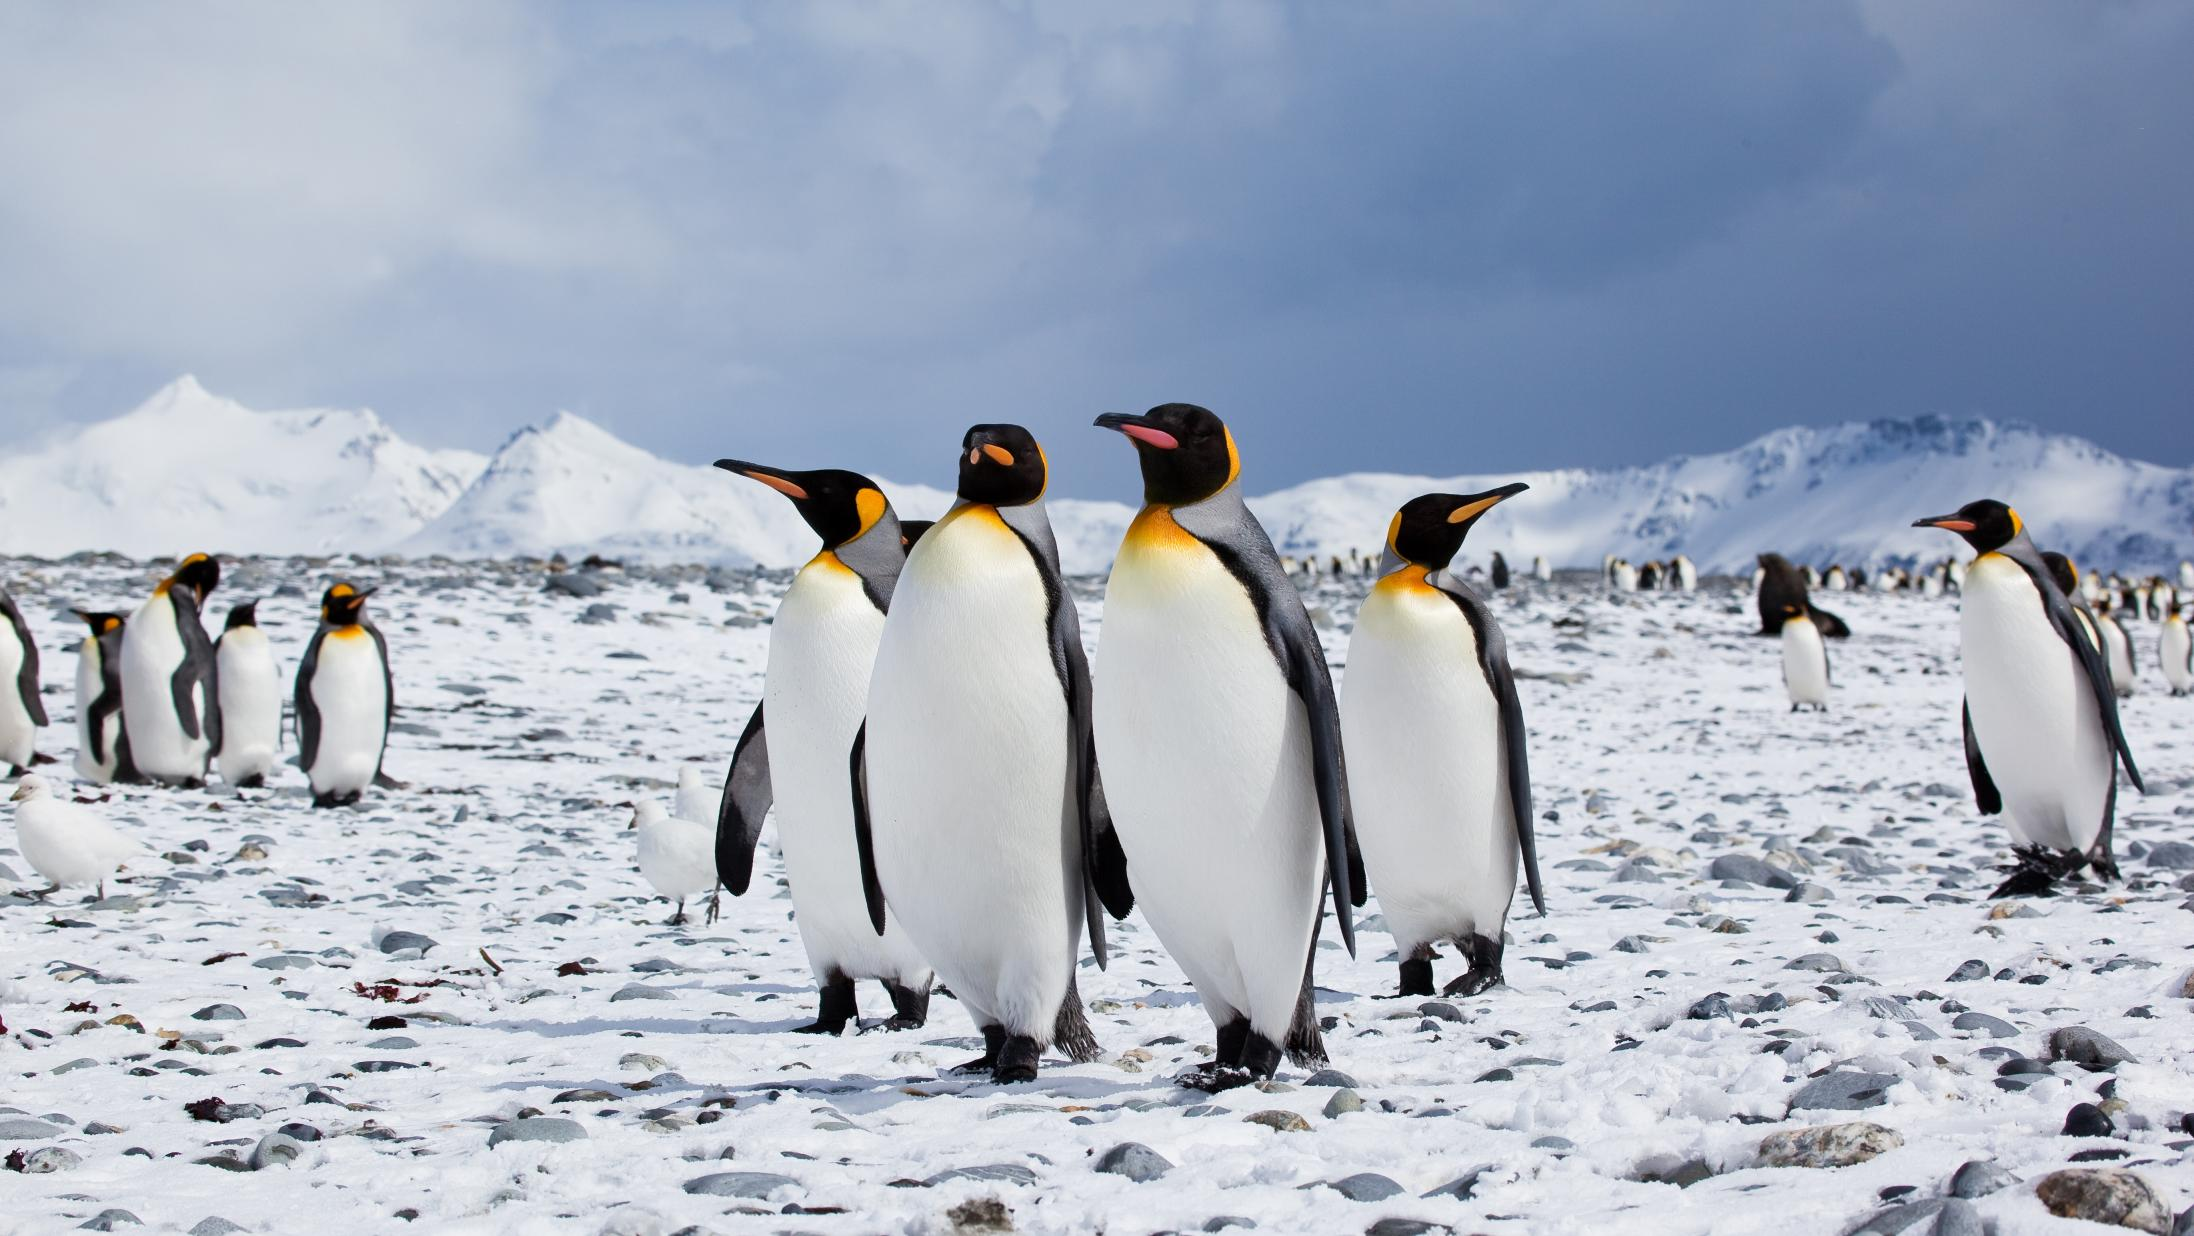
\includegraphics[width=\linewidth]{graphI-08-penguins.jpg}}{Source : \href{https://www.flickr.com/photos/antarcticabound/5220534077/}{Flickr CC By-ND 2.0}}
D’un ordinateur ou d’une tablette, on distingue d’abord l’écran et le boîtier qui enferme le matériel --- processeurs, mémoires et canaux d’entrées-sorties ---, mais c’est le logiciel qu’il contient que l’on utilise.

La programmation directe de l’ordinateur est laborieuse. La machine, construite sur le modèle de \textsc{von Neumann}, est universelle (voir sur \href{https://interstices.info/}{Interstices} « \href{https://interstices.info/sous-le-signe-du-calcul/}{\textit{Sous le signe du calcul}} », par Jean-Louis \textsc{Giavitto} et François \textsc{Rechenmann} et « \href{https://interstices.info/alan-turing-du-concept-a-la-machine/}{\textit{Alan \textsc{Turing} : du concept à la machine}} », par Sacha \textsc{Krakowiak}). Toutefois, le langage qu’elle reconnaît, composé d’instructions et de données, toutes codées en binaire, est très difficile d’emploi. Le système d’exploitation vient alors au secours de l’utilisateur, en lui permettant d’exploiter l’ordinateur mieux qu’en langage machine. Mais il fait plus que cela.

\overparagraph{Rôles du système d’exploitation}

Le but d’un système d’exploitation est de rendre aisée l’utilisation de l’ordinateur par chacun, comme s’il s’agissait d’une machine fictive, sa « machine virtuelle », qui aurait été construite pour lui. Le système fournit un accès commode et ergonomique, par exemple avec un écran comportant des fenêtres multiples et une interface graphique. De nos jours, en 2015, il peut aussi y avoir une interface tactile ou sonore.\nopagebreak

Le système assure ainsi le stockage de programmes et de données de toutes sortes --- textes, images, vidéos, films --- \pagebreak dans des fichiers préparés par l’utilisateur ou chargés depuis des supports externes ou \textit{via} le réseau. Idéalement, ce premier rôle de gestion de l’information et des fichiers doit permettre à l’utilisateur de n’avoir à préciser que les aspects logiques de son travail.

\sidegraphic*{%
%
\includegraphics[height=2.4cm]{./Images/Logotype/tux-869-1024px.png}\\[\baselineskip]
%
\includegraphics[height=2.0cm]{./Images/Logotype/apple-logo-black-1024px.png}\\[\baselineskip]
%
\includegraphics[height=2.0cm]{./Images/Logotype/windows-logo-2012-derivative-multicolor-1024px.png}\\[\baselineskip]
%
\includegraphics[height=2.0cm]{./Images/Logotype/android-robot-1024px.png}

\includegraphics[width=0.3333\linewidth]{./Images/Logotype/linux-tux-logo-1024px.png}\\[\baselineskip]

\includegraphics[width=0.3333\linewidth]{./Images/Logotype/apple-logo-black-1024px.png}\\[\baselineskip]

\includegraphics[width=0.3333\linewidth]{./Images/Logotype/windows-logo-2012-derivative-multicolor-1024px.png}\\[\baselineskip]

\includegraphics[width=0.3333\linewidth]{./Images/Logotype/android-robot-1024px.png}
}
%\sidegraphic*{
\includegraphics[width=.5\linewidth]{./Images/Logotype/tux-869-1024px.png}\\[\baselineskip]
%
\includegraphics[width=.5\linewidth]{./Images/Logotype/apple-logo-black-1024px.png}\\[\baselineskip]
%
\includegraphics[width=.5\linewidth]{./Images/Logotype/windows-logo-2012-derivative-multicolor-1024px.png}\\[\baselineskip]
%
\includegraphics[width=.5\linewidth]{./Images/Logotype/android-robot-1024px.png}
%}
%\sidegraphic*{
\includegraphics[width=.5\linewidth]{./Images/Logotype/apple-logo-black-1024px.png}}
%\sidegraphic*{
\includegraphics[width=.5\linewidth]{./Images/Logotype/windows-logo-2012-derivative-multicolor-1024px.png}}
Le second rôle du système, le contrôle d’exécution, consiste à gérer au mieux les ressources --- matérielles et logicielles --- qui sont nécessaires pour lancer et suivre l’exécution des applications locales ou distantes. Le système s’occupe ainsi des aspects technologiques et des contraintes d’utilisation des ressources partagées, qu’elles soient attribuées à tour de rôle, comme le sont le processeur et l’imprimante ou divisées, comme le sont la mémoire et l’écran.

Ces deux rôles doivent être pérennes. Pour cela, le système d’exploitation assure --- et c’est là son troisième rôle --- la sécurité de fonctionnement en cas de panne d’origine interne (matérielle ou logicielle) ou d’agression provenant d’un environnement de plus en plus ouvert (le réseau). Il sauvegarde automatiquement les travaux en cours et veille à permettre le redémarrage après une panne. Il doit aussi rendre possible une évolution matérielle (changement dans la configuration matérielle) ou fonctionnelle (mise à jour et ajout de programmes).

Ces rôles sont remplis par des services décrits dans les programmes du système d’exploitation ; l’exécution de ces programmes --- et donc des services --- est accomplie par ses processus.

Un programme est une entité passive, décrivant une suite d’instructions. Un processus est son pendant dynamique, une entité active qui représente l’exécution de cette suite d’instructions par l’ordinateur.

\overparagraph{Représentations du système d’exploitation}

Dans sa mouture générique, un système d’exploitation peut s'appréhender selon deux aspects :
\begin{itemize}
\item une vision « statique » qui correspond à l’empilement hiérarchique de ses programmes ;
\item une perspective « dynamique » qui rend compte de l’exécution des programmes par les processus.
\end{itemize}

\begin{marginfigure}
	\begin{tikzpicture}[scale=1.0, inner sep=0pt, outer sep=0pt]
		%\draw [very thin, lightgray] (0,0) grid[step=0.2] (5,6);
		%\draw [very thin, gray] (0,0) grid (5,6);
		%\node[inner sep=0pt, outer sep=0pt] at (0,0) {\includegraphics[width=\marginparwidth]{example-image-a}};
		%\node[font=\footnotesize, yshift=1.5cm, text=secondcolor, inner sep=0pt, outer sep=0pt] 
		%	(staticOS) at (0,0) {\textbf{Faire un schéma...}};
		\node[rectangle, draw=firstcolor, fill=gray!40,
					line width=0.8pt, label=center:\textsc{\lightbf{\footnotesize Interfaces physiques, noyau exécutif}},
					minimum width=(\marginparwidth-0.8pt), minimum height=0.75cm] (rect1) at (0,0) {};
		\node[rectangle, draw=firstcolor, fill=gray!20,
					line width=0.8pt, label=center:\textsc{\lightbf{\footnotesize Pilotes des ressources physiques}},
					minimum width=(\marginparwidth-0.8pt), minimum height=0.75cm] (rect2) at (0,0.75cm) {};
		\node[rectangle, draw=firstcolor, fill=gray!40,
					line width=0.8pt, label=center:\textsc{\lightbf{\footnotesize Services du système d'exploitation}},
					minimum width=(\marginparwidth-0.8pt), minimum height=0.75cm] (rect3) at (0,1.5cm) {};
		\node[rectangle, draw=firstcolor, fill=gray!20,
					line width=0.8pt, label=center:\textsc{\lightbf{\footnotesize Services communautaires}},
					minimum width=(\marginparwidth-0.8pt), minimum height=0.75cm] (rect4) at (0,2.25cm) {};
		\node[rectangle, draw=firstcolor, fill=gray!40,
					line width=0.8pt, label=center:\textsc{\lightbf{\footnotesize Programmes d'application}},
					minimum width=(\marginparwidth-0.8pt), minimum height=0.75cm] (rect4) at (0,3.0cm) {};
	\end{tikzpicture}
\caption{\label{fig:I.8}Représentation statique du système d'exploitation : descriptif et approche en couches (cf. \href{https://interstices.info/a-quoi-sert-un-systeme-dexploitation/}{Interstices}).}
\end{marginfigure}

\paragraph*{Représentation statique : les programmes}
Le systè\-me d’exploitation d’un ordinateur est un fantastique regroupement de programmes et de données qui ont été élaborés pour fournir les services requis pour chacun des rôles cités précédemment. Ces informations sont empilées astucieusement en couches qui reflètent la forte structuration de la construction : au niveau le plus bas, on trouve les programmes du noyau qui matérialisent les principes sur lesquels la construction du système est fondée, puis les programmes qui pilotent l’accès au matériel ; au-dessus, dans l’ordre ascendant, utilisant parfois les programmes des couches qui leur sont sous-jacentes, viennent les services propres du système d’exploitation, les services communautaires et, enfin, les programmes d’application destinés à l’utilisateur. La \cref{fig:I.8} schématise la représentation habituelle de ces services.

Cet empilement structuré d’informations forme une grande base de données : les fichiers du système. Il faut y ajouter les fichiers des utilisateurs entreposés sur des supports gérés par le système d’exploitation ou accessibles à distance sur le réseau.

La rapidité des processeurs et la grande capacité de la mémoire permettent de construire des systèmes très complexes et de taille considérable qui peut atteindre une dizaine de\caution[t]{Lien mort : \url{https://interstices.info/jcms/c_19937/octet}.} \href{https://interstices.info/jcms/c_19937/octet}{gigaoctets}. Par exemple, un système d’exploitation utilisé pour un ordinateur portable, le système d’exploitation MacOSX 10.6, occupe environ $5$\,Go en mémoire, auxquels s’ajoutent de $5$ à $15$\,Go pour les bibliothèques partagées.

\paragraph*{Représentation dynamique : les processus}

De nombreux programmes du système qui ont leurs sources --- codes et données --- dans ces empilements de couches sont appelés à s’exécuter de façon concomitante. Ils répondent en temps réel aux besoins explicites ou implicites des utilisateurs et réagissent aux événements aléatoires issus de l’environnement. Quelquefois, c’est le même service qui est demandé simultanément par plusieurs événements ou utilisateurs. Le système d’exploitation peut ainsi être amené à gérer l’exécution concurrente de plusieurs centaines de programmes. Le mot concurrent, polysémique, évoque à la fois la simultanéité --- les programmes courent ensemble --- et la compétition dans l’attribution des ressources.

\begin{marginfigure}
	\begin{tikzpicture}[scale=1.0, inner sep=0pt, outer sep=0pt]
		%\draw [very thin, lightgray] (0,0) grid[step=0.2] (5,6);
		%\draw [very thin, gray] (0,0) grid (5,6);
		%\node[inner sep=0pt, outer sep=0pt] at (0,0) {\includegraphics[width=\marginparwidth]{example-image-a}};
		%\node[font=\footnotesize, yshift=1.5cm, text=secondcolor, inner sep=0pt, outer sep=0pt] 
		%	(staticOS) at (0,0) {\textbf{Faire un schéma...}};
		%\draw[-stealth] (0,1) arc [start angle=0, end angle=360, radius=1cm];
		\begin{scope}[yshift=2.5cm]
			\draw[Latex-, fill=gray!60] (-1.3125,0.375) arc [start angle=90, end angle=450, radius=0.25cm];
			\draw[Latex-, fill=gray!20] (-0.65625,0.375) arc [start angle=90, end angle=450, radius=0.25cm];
			\draw[Latex-, fill=gray!60] (0,0.375) arc [start angle=90, end angle=450, radius=0.25cm];
			\draw[Latex-, fill=gray!20] (0.65625,0.375) arc [start angle=90, end angle=450, radius=0.25cm];
			\draw[Latex-, fill=gray!60] (1.3125,0.375) arc [start angle=90, end angle=450, radius=0.25cm];
			\node[rectangle, draw=firstcolor, fill=none,%gray!40, line width=0.8pt,
						line width=0.8pt, minimum width=(\marginparwidth-0.8pt), minimum height=1.25cm] (rect1) at (0,0.0) {}; 
			\node[align=center,yshift=0.25cm] at (rect1.south) {\textsc{\lightbf{\footnotesize Processus des utilisateurs}}};
		\end{scope}
		\begin{scope}[yshift=1.25cm]
			\draw[Latex-, fill=gray!60] (-1.3125,0.375) arc [start angle=90, end angle=450, radius=0.25cm];
			\draw[Latex-, fill=gray!20] (-0.9375,0.375) arc [start angle=90, end angle=450, radius=0.25cm];
			\draw[Latex-, fill=gray!60] (-0.5625,0.375) arc [start angle=90, end angle=450, radius=0.25cm];
			\draw[Latex-, fill=gray!20] (-0.1875,0.375) arc [start angle=90, end angle=450, radius=0.25cm];
			\draw[Latex-, fill=gray!60] (0.1875,0.375) arc [start angle=90, end angle=450, radius=0.25cm];
			\draw[Latex-, fill=gray!20] (0.5625,0.375) arc [start angle=90, end angle=450, radius=0.25cm];
			\draw[Latex-, fill=gray!60] (0.9375,0.375) arc [start angle=90, end angle=450, radius=0.25cm];
			\draw[Latex-, fill=gray!20] (1.3125,0.375) arc [start angle=90, end angle=450, radius=0.25cm];
			\node[rectangle, draw=firstcolor, fill=none,%gray!40, line width=0.8pt,
						line width=0.8pt, minimum width=(\marginparwidth-0.8pt), minimum height=1.25cm] (rect2) at (0,0.0) {}; 
			\node[align=center,yshift=0.25cm] at (rect2.south) {\textsc{\lightbf{\footnotesize Processus du système}}};
		\end{scope}
		\begin{scope}[yshift=0.0cm]
			\draw[Latex-, fill=gray!60] (-0.65625,0.375) arc [start angle=90, end angle=450, radius=0.25cm];
			\draw[Latex-, fill=gray!20] (0,0.375) arc [start angle=90, end angle=450, radius=0.25cm];
			\draw[Latex-, fill=gray!60] (0.65625,0.375) arc [start angle=90, end angle=450, radius=0.25cm];

			\node[rectangle, draw=firstcolor, fill=none,%gray!40, line width=0.8pt,
						line width=0.8pt, minimum width=(\marginparwidth-0.8pt), minimum height=1.25cm] (rect3) at (0,0.0) {}; 
			\node[align=center,yshift=0.25cm] at (rect3.south) {\textsc{\lightbf{\footnotesize Processeurs}}};
		\end{scope}
	\end{tikzpicture}
\caption{\label{fig:I.9}Représentation dynamique du système d'exploitation : descriptif et approche en processus (cf. \href{https://interstices.info/a-quoi-sert-un-systeme-dexploitation/}{Interstices}).}
\end{marginfigure}

Afin de repérer ces différentes exécutions concomitantes, le terme de processus a été introduit. Ce mot a été utilisé dès 1960 dans le système \textsc{Multics}. Il sert à identifier le déroulement d’un programme séquentiel ---  parmi d’autres --- et le distingue du texte du programme. 
%\url{https://interstices.info/encart.jsp?id=p_83884&encart=1&size=600,500}% lien mort

La \cref{fig:I.9} schématise cette vision dynamique, qui traduit l’activité des processus. On y distingue les processus du système, à savoir les processus chargés des infrastructures et des services communautaires et les processus créés plus spécialement pour fournir une « machine virtuelle » à chaque utilisateur. Chacun des processus est une abstraction du processeur physique.

\overparagraph{Processus et processeurs}

\begin{marginfigure}
	%\newdimen{\labelwidth}%
	%\settowidth{\labelwidth}{\scriptsize Processus 1}%
	%\begin{tikzpicture}[yscale=0.6666]%[scale=1.0, inner sep=0pt, outer sep=0pt]
	\begin{tikzpicture}[xscale=0.995, yscale=0.6666]%[scale=1.0, inner sep=0pt, outer sep=0pt]
		%\draw [very thin, lightgray] (0,0) grid[step=0.2] (5.2,6);
		%\draw [very thin, gray] (0,0) grid (5.2,6);
		%\node[inner sep=0pt, outer sep=0pt] at (0,0) {\includegraphics[width=\marginparwidth]{example-image-a}};
		%\node[font=\footnotesize, yshift=1.5cm, text=secondcolor, inner sep=0pt, outer sep=0pt] 
		%	(staticOS) at (0,0) {\textbf{Faire un schéma...}};
		%\draw[-stealth] (0,1) arc [start angle=0, end angle=360, radius=1cm];
		\node[align=left, anchor=west, inner sep=0pt, outer sep=0pt] (processus1) at (0.0,5.0) {\scriptsize Processus 1};
		\draw[draw=gray!80, line width=1.2pt] (1.4,5.0) -- (\marginparwidth,5.0);
		\draw[draw=black, line width=2.4pt] (1.40,5.0) -- (1.80,5.0);
		\draw[draw=black, line width=2.4pt] (3.40,5.0) -- (3.80,5.0);
		\draw[draw=black, line width=2.4pt] (4.90,5.0) -- (5.20,5.0);
		\node[align=left, anchor=west, inner sep=0pt, outer sep=0pt] (processus2) at (0.0,4.0) {\scriptsize Processus 2};
		\draw[draw=gray!80, line width=1.2pt] (1.4,4.0) -- (\marginparwidth,4.0);
		\draw[draw=black, line width=2.4pt] (2.90,4.0) -- (3.25,4.0);
		\draw[draw=black, line width=2.4pt] (3.95,4.0) -- (4.25,4.0);
		\node[align=left, anchor=west, inner sep=0pt, outer sep=0pt] (processus3) at (0.0,3.0) {\scriptsize Processus 3};
		\draw[draw=gray!80, line width=1.2pt] (1.4,3.0) -- (\marginparwidth,3.0);
		\draw[draw=black, line width=2.4pt] (1.95,3.0) -- (2.30,3.0);
		\draw[draw=black, line width=2.4pt] (4.40,3.0) -- (4.75,3.0);
		\node[align=left, anchor=west, inner sep=0pt, outer sep=0pt] (processus4) at (0.0,2.0) {\scriptsize Processus 4};
		\draw[draw=gray!80, line width=1.2pt] (1.4,2.0) -- (\marginparwidth,2.0);
		\draw[draw=black, line width=2.4pt] (2.45,2.0) -- (2.75,2.0);
		\node[align=left, anchor=west, inner sep=0pt, outer sep=0pt] (kernel) 
			at (0.0,1.0) {\scriptsize Noyau\\[-0.6ex]\scriptsize  du système};
		\draw[draw=gray!80, line width=1.2pt] (1.4,1.0) -- (\marginparwidth,1.0);
		\draw[draw=black, line width=2.4pt] (1.80,1.0) -- (1.95,1.0);
		\draw[draw=black, line width=2.4pt] (2.30,1.0) -- (2.45,1.0);
		\draw[draw=black, line width=2.4pt] (2.75,1.0) -- (2.90,1.0);
		\draw[draw=black, line width=2.4pt] (3.25,1.0) -- (3.40,1.0);
		\draw[draw=black, line width=2.4pt] (3.80,1.0) -- (3.95,1.0);
		\draw[draw=black, line width=2.4pt] (4.25,1.0) -- (4.40,1.0);
		\draw[draw=black, line width=2.4pt] (4.75,1.0) -- (4.90,1.0);
		\node[align=left, anchor=west, inner sep=0pt, outer sep=0pt] (processor) at (0.0,0.0) {\scriptsize Processeur};
		\draw[draw=black, line width=2.4pt] (1.4,0.0) -- (\marginparwidth,0.0);
		\draw[-Latex, draw=secondcolor] (1.80,5.0) -- (1.800,1.0);
		\draw[-Latex, draw=firstcolor] (1.95,1.0) -- (1.95,3.0);
		\draw[-Latex, draw=secondcolor] (2.30,3.0) -- (2.30,1.0);
		\draw[-Latex, draw=firstcolor] (2.45,1.0) -- (2.45,2.0);
		\draw[-Latex, draw=secondcolor] (2.75,2.0) -- (2.75,1.0);
		\draw[-Latex, draw=firstcolor] (2.90,1.0) -- (2.90,4.0);
		\draw[-Latex, draw=secondcolor] (3.25,4.0) -- (3.25,1.0);
		\draw[-Latex, draw=firstcolor] (3.40,1.0) -- (3.40,5.0);
		\draw[-Latex, draw=secondcolor] (3.80,5.0) -- (3.80,1.0);
		\draw[-Latex, draw=firstcolor] (3.95,1.0) -- (3.95,4.0);
		\draw[-Latex, draw=secondcolor] (4.25,4.0) -- (4.25,1.0);
		\draw[-Latex, draw=firstcolor] (4.40,1.0) -- (4.40,3.0);
		\draw[-Latex, draw=secondcolor] (4.75,3.0) -- (4.75,1.0);
		\draw[-Latex, draw=firstcolor] (4.90,1.0) -- (4.90,5.0);
		%- Légendes
		\draw[-Latex, draw=secondcolor, anchor=west] (0.1,-0.75) -- (0.5,-0.75);
		\node[anchor=west] at (0.6,-0.75) {\scriptsize Interruption d'horloge};
		\draw[-Latex, draw=firstcolor, anchor=west] (0.1,-1.25) -- (0.5,-1.25);
		\node[anchor=west] at (0.6,-1.25) {\scriptsize Choix de l’ordonnanceur};
		\draw[draw=black, line width=2.4pt, anchor=west] (0.1,-1.75) -- (0.5,-1.75);
		\node[anchor=west] at (0.6,-1.75) {\scriptsize Utilisation séquentielle du processeur};
	\end{tikzpicture}
\caption{\label{fig:I.10}Processeur partagé, prêté successivement à quatre processus (cf. \href{https://interstices.info/a-quoi-sert-un-systeme-dexploitation/}{Interstices}).}
\end{marginfigure}

La représentation dynamique fait apparaître une nuée de processus, alors qu’il n’y a pas assez de processeurs physiques pour en attribuer un à chacun. Or les processeurs physiques ont une vitesse environ un million de fois supérieure à la capacité de réaction de l’utilisateur. Cette énorme différence est mise à profit pour simuler le parallélisme de déroulement des programmes en partageant les processeurs entre les processus --- appelé le pseudo‑parallélisme. Le partage est rythmé par un top d’horloge qui déclenche l’interruption du processus en cours et l’attribution du processeur à un autre processus. Cette attribution est régie par un programme du noyau du système, l’ordonnanceur.

%La représentation dynamique fait apparaître une nuée de processus, alors même qu’il n’y a pas assez de processeurs physiques pour en attribuer un à chacun. Or les processeurs physiques ont une vitesse environ un million de fois supérieure à la capacité de réaction de l’utilisateur. Cette énorme différence de rapidité est mise à profit pour simuler le parallélisme de déroulement des programmes en partageant les processeurs entre les processus --- c’est ce qu’on appelle le pseudo‑parallélisme. Le partage est rythmé par un top d’horloge qui déclenche l’interruption du processus en cours et l’attribution du processeur à un autre processus. Cette attribution est régie par un programme du noyau du système, l’ordonnanceur.

La figure \cref{fig:I.10} montre un exemple de partage d’un processeur (on suppose ici qu’il n’y en a qu’un) entre quatre processus déclenchés simultanément qui l’utilisent l’un après l’autre, par tranches séquentielles successives. L’attribution du processeur par le noyau consomme aussi du temps de processeur.

\overparagraph{Bilan}

La complexité des systèmes d’exploitation est grande, elle résulte tant du nombre et de la taille des programmes impliqués, que de la multiplicité des processus et de leurs interactions. Cette grande complexité rend illusoire le « zéro défaut » ! 

Aujourd'hui, on continue de développer de nouveaux systèmes, tout en recherchant l’augmentation de leur sûreté de fonctionnement. Pour cela, on commence à utiliser des techniques automatiques de certification de programmes.\caution[c]<firstcolor>{Pour comprendre dans le détail la dynamique d’un système d’exploitation et\linebreak découvrir les processus qui se déclen\-chent lors du lancement d’un ordinateur, le lecteur est invité à consulter l’article « \href{https://interstices.info/le-ballet-des-processus-dans-un-systeme-dexploitation/}{\textit{Le ballet des processus dans un système d'exploitation}} », Interstices, 2015.}{Complément de lecture}

\begin{gofurther}[after skip=2pt]
\textsc{\lightbf{Métaphore badine}}
\begin{itemize}\jazzitem
\item \href{https://interstices.info/de-votre-boulangerie-a-un-systeme-dexploitation-multiprocesseur/}{De votre boulangerie à un système d'exploitation multiprocesseur}, par Brice \textsc{Goglin}, Interstices, 15 février 2011.
\end{itemize}

\smallskip
\textsc{\lightbf{Quelques aspects historiques}}
\begin{itemize}\jazzitem
\item \href{https://interstices.info/la-naissance-des-systemes-dexploitation/}{Naissance des systèmes d'exploitation}, par Sacha \textsc{Krakowiak} et Jacques \textsc{Mossière}, Interstices, 5 avril 2013 ;
\item \href{https://interstices.info/les-debuts-dune-approche-scientifique-des-systemes-dexploitation/}{Débuts d’une approche scientifique des systèmes d’exploitation}, par Sacha \textsc{Krakowiak}, Interstices, 03 février 2014 ;
\item \href{https://fr.wikipedia.org/wiki/Liste_des_syst\%C3\%A8mes_d\%27exploitation}{Liste des systèmes d'exploitation} maintenue sur Wikipédia. Pour les systèmes \textsc{GNU/Linux}, se référer à \href{https://distrowatch.com/}{DistroWhatch}.
\end{itemize}

\smallskip
\textsc{\lightbf{Apprendre \textsc{Linux}}}
\begin{itemize}\jazzitem
\item \textsc{OpenClassrooms} propose un \href{https://openclassrooms.com/fr/courses/43538-reprenez-le-controle-a-laide-de-linux}{cours pour débuter en Linux}.
\end{itemize}

\smallskip
\textsc{\lightbf{Comment créer son propre système d'exploitation ?}}
\begin{itemize}\jazzitem
\item \href{http://a.michelizza.free.fr/}{Apprendre à programmer son propre noyau de système d'exploitation : une introduction avec Pépin}, page en français qui date un peu, mais néanmoins relativement complète ;
\item \href{https://wiki.osdev.org/Main_Page}{OSDev.org}, site dédié à la création de SE/OS ;
\item \href{https://studioexpress.opensuse.org/}{Suse Studio}, pour créer une distribution \textsc{Linux} (bien d'autres solutions existent sur des bases différentes, se fondant sur \href{https://www.debian.org/index.fr.html}{\textsc{Debian}}, \href{https://ubuntu.com/}{\textsc{Ubuntu}} ou autres, \href{https://www.gentoo.org/}{\textsc{Gentoo}} et \href{https://www.archlinux.org/}{\textsc{ArchLinux}}).
\end{itemize}
\end{gofurther}


%----------
\section[Interface humain-machine]{Interface humain-machine}
\label{sec:I.3}

\vspace*{-2pt}
\caution[t]<secondcolor>{%
Anke \textsc{Brock} est chargée de recherche de l'équipe-projet \href{https://team.inria.fr/potioc/fr/}{\textsc{Potioc}} au centre de recherche \textsc{Inria} \textsc{Bordeaux--Sud-Ouest}. Née en Allemagne, elle a travaillé cinq ans dans un département de recherche et développement dans l'industrie automobile avant de rejoindre la France. À l'\textsc{Inria}, elle œuvre dans le domaine de l'interaction Homme-Machine et se consacre désormais au développement de son propre projet de recherche : l'interaction avec les cartes géographiques.}{À propos de l'intervenante}
Comment les humains interagissent-ils avec les machines (ordinateur, \textit{smartphone}, etc.) ? Comment concevoir des systèmes à la fois efficaces, efficients et satisfaisants pour leurs utilisateurs ? 

Voici donc les questions que posent ce domaine particulier de recherche qu'est l'\textsc{Ihm} --- \gls{IHM}, Interaction humain-machine ---, qui s'intéresse à la conception de systèmes de relation, comme son nom l'indique, entre humains et machines.

De fait, l'\textsc{Ihm} est une spécialité partie prenante de l'informatique, mais elle intègre également des disciplines comme, entre autres, les \gls{cognitivesciences}, l'\gls{ergonomics}, le \gls{design} et l'électronique. 

Les champs d'investigation comportent principalement deux axes :
\begin{enumerate}
\item le premier est de concevoir, d'observer, d'analyser et d'évaluer l'interaction et l'expérience des humains avec les technologies ;
\item le second est plus technique : il s'agit d'envisager et d'élaborer les environnements existants et futurs, tout en appréciant leur évolution en fonction de l'interaction qu'ils ont avec les humains. 
\end{enumerate}

\vspace*{-2pt}
\subsection[Interactivité]{Interactivité}
\label{sub:I.3.1}

\begin{marginvideo}
	[\label{vid:I.4}Interface Humain-Machine I.]%
	\vspace*{-36pt}%
	\movie[width=\marginparwidth,showcontrols]%
		{
\includegraphics[width=\marginparwidth]{./Images/Pictograms/film-strip-dark-electric-blue.png}}%
		{./Videos/Chapter01/vidI-04-IHM-01-HD.mp4}%
	\launchvideo{./Videos/Chapter01/vidI-04-IHM-01-HD.mp4}
\end{marginvideo}

Interagir avec des technologies apporte des besoins nouveaux, lesquels stimulent à leur tour de nouvelles mutations. À titre d'illustration, la majorité 
des gens possède aujourd'hui un téléphone intelligent connecté à l'Internet. Les plus ou moins jeunes ont peut-être du mal à se départir des réseaux sociaux ; cela s'avère quelque chose que la génération précédente n'aurait même pas pu imaginer.

Cette utilisation induit de nouvelles évolutions technologiques, qui conduisent alors à des solutions encore plus portables, plus petites, comme des bracelets électroniques ou des montres intelligentes, voire des puces électroniques greffées au corps.

Néanmoins, au-delà des questions de philosophie et d'éthique posées, cela rend bien d'autres services et présente des intérêts utiles en termes de thématiques de recherche, comme l'accessibilité des terminaux aux personnes en situation de handicap ou l'interaction avec un ordinateur qui ne possède plus du tout d'écran, ni encore de clavier.

\nopagebreak

%\vspace*{-4pt}
\subsubsection[Bref historique]{Bref historique}
\label{subsub:I.3.1.1}

Les interfaces humain-machine apparaissent vraiment dans les années 1980, car l'informatique est auparavant réservée aux \pagebreak professionnels. % de ce domaine d'exercice.
C'est effectivement avec les ordinateurs personnels, alors orientés sur la bureautique, les jeux interactifs et la MAO\sidenote{Notamment l'\href{https://fr.wikipedia.org/wiki/Atari_ST}{\textsc{Atari ST}} lancé en 1985.} --- Musique assistée par ordinateur ---, qu'émergent les premières interfaces graphiques «~tout public~» et normalisations de format de données comme le MIDI --- \textit{Musical Instrument Digital Interface} (1983).
\sidegraphic*[Triplet classique des ports MIDI IN, OUT et THRU en connectique DIN.]{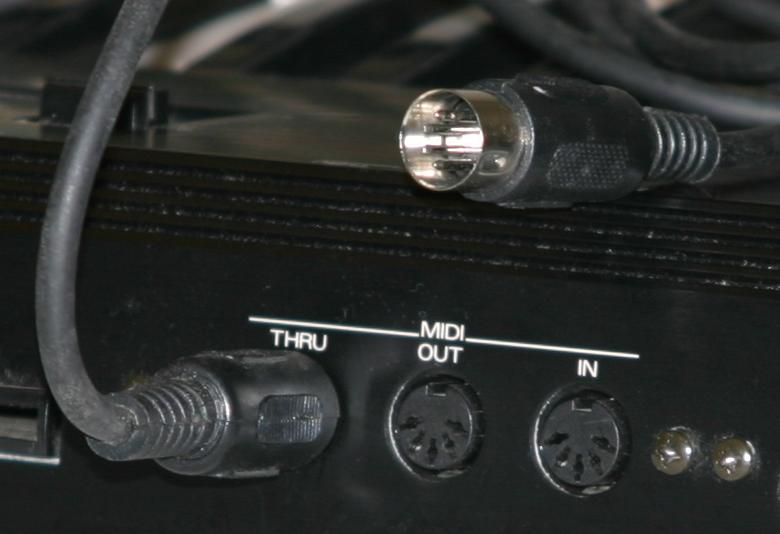
\includegraphics[width=\linewidth]{graphI-09-midi-ports-cable.jpg}}{Source : \href{https://fr.wikipedia.org/wiki/Musical_Instrument_Digital_Interface}{Wikipedia \faWikipediaW}}

À cette époque, « tout\sidenote{À condition toutefois d'y consacrer un budget relativement conséquent pour le quidam moyen. La calculatrice programmable fut d'abord l'apanage des \textit{geeks} en herbe des cours d'école au tournant des décennies 1970-1980, \textsc{Texas Instrument} se taillant alors la part belle.} le monde » devient donc un utilisateur potentiel de l'ordinateur. Cela conduit à révéler les problèmes et limites d'utilisabilité de ces machines à grande échelle. En parallèle et dans le même temps, se développent des disciplines comme les \gls{cognitivesciences}, fondées sur la \gls{cognitivepsychology}, l'\gls{AI} ou encore la \gls{linguistics} et la philosophie.

Nombre de domaines ont été impactés par l'avènement des ordinateurs. On a ainsi assisté aux premiers efforts de simulation numérique et de concepts mathématiques\sidenote{Nouveau champ de recherche des mathématiques : l'analyse numérique.} sous-jacents.
Mais aussi et, posant derechef la question d'une interface adaptée, les premières tentatives de synthétiseurs musicaux\sidenote{Au-delà des méthodes de synthèse sonore purement mathématiques des années 1960, \textsc{Hiller} et \textsc{Ruiz}, dès 1970, utilisent l'ordinateur pour simuler la vibration d'une corde \jazzcite{Ruiz:1970}, \jazzcite{HillerRuiz:1971}.} se sont faits jour. Avant de se généraliser à d'autres instruments électroniques, l'interface de prédilection fut d'abord un clavier... Cette fois musical, clone de celui d'un piano.

Avec la complexité croissante des logiciels et la nécessité de tenir compte du facteur humain dès la conception même d'un système d'information, les industries comme l'avionique et l'automobile --- et plus largement la fabrication assistée par ordinateur ---, mais encore des applications de la société civile comme l'\gls{accessibility} aux personnes âgées ou bien en situation de handicap, vont intégrer progressivement nombre de concepts d'interaction humain-machine comme la visualisation des données et des résultats, les systèmes collaboratifs directs ou \textit{via} Internet (décennie 1990) et, plus récemment, les \glspl{ubiquitoussystem}\sidenote{Portail \href{https://www.cnrtl.fr/}{\textsc{Cnrtl}}, \href{https://www.cnrtl.fr/definition/ubiquitaire}{\textit{ubiquitaire}} [adj.] : « Qui manifeste la faculté qu'une personne [un objet] possède de se trouver en différents endroits à la fois ».} ou encore les procédures\sidenote{Méthodes itératives (cf. infra) --- entre l'utilisateur et le programmeur ---, de développement des logiciels avec, aujourd'hui, les méthodes dites « \href{https://fr.wikipedia.org/wiki/M\%C3\%A9thode_agile}{agiles} ».} de conception.

%\vspace*{-4pt}
\subsubsection[Concept d'utilisabilité]{Concept d'utilisabilité}
\label{subsub:I.3.1.2}

L'\emph{\gls{usability}} est un concept fondamental du champ sémantique de l'interaction homme--machine. Au début, on signifiait vaguement qu'un système soit utilisable quand il était facile à apprendre et à manipuler. Par la suite, ce concept a été élargi. 

Plusieurs normes ISO définissent l'\gls{usability}, dont par exemple la \gls{ISO9241-2010}, qui stipule que l'\gls{usability} est «~\textit{le degré selon lequel un produit peut être utilisé par des utilisateurs identifiés pour atteindre des buts définis avec \gls{effectiveness}, \gls{efficiency} et \gls{satisfaction} dans un contexte d'utilisation spécifié}~». Cette définition est assez complexe. Elle est décomposée pour appréhender séparément les concepts :

\begin{description}
	\item[Efficacité] --- L'\gls{effectiveness} est la précision et le degré d'achèvement selon lesquels l'utilisateur atteint des objectifs spécifiques. Autrement dit, un système est efficace s'il permet à un utilisateur d'effectuer les tâches qu'il a envie ou besoin de faire.
	\item[Efficience] --- L'\gls{efficiency} est le rapport entre les ressources dépensées et la précision ou le degré 
d'achèvement selon lesquels l'utilisateur atteint les objectifs attendus. Plus précisément, un système rapide à manipuler et ne demandant pas beaucoup d'interactions va être plus efficient que celui où l'utilisateur a besoin de passer beaucoup de temps pour atteindre ces objectifs.
	\item[Satisfaction] --- La \gls{satisfaction} caractérise les attitudes positives du maniement d'un produit ; l'utilisateur prend-il plaisir à l'employer ?
\end{description}

Ainsi, \textit{pour qu'un produit soit utilisable, il faut à la fois qu'il soit efficace, efficient et satisfaisant}. Cette assertion est fondamentale car, même un algorithme ultra performant ne sera pas adopté si son interface est conçue d'une manière qui ne respecte pas ces critères.

\sidegraphic*{
\includegraphics[width=0.6\linewidth]{./Images/Logotype/iso-logo-1024px.png}}
La norme ISO indique en outre que l'utilisabilité est définie en fonction des \emph{utilisateurs} et des \emph{contextes}.
Pour concevoir des systèmes informatiques, il semble logique de les définir selon leur \emph{cible}, à savoir les \emph{utilisateurs finaux}. Cela peut concerner des attributs d'âge --- enfants ou anciens ---, devoir répondre à des besoins particuliers --- malvoyants ou handicaps divers --- ou bien encore, tenir compte des connaissances et compétences antérieures --- néophytes \textit{versus} aguerris. 

\emph{On ne conçoit pas un système informatique de la même manière pour le grand public que pour des professionnels et des experts}.

\paragraph*{Système d'aide à la navigation aérienne}
Un pilote d'avion ou encore un contrôleur aérien a besoin d'un système d'information qui ne fasse pas d'erreur : il doit être absolument fiable. Les critères d'efficacité et d'efficience vont donc être essentiels. En revanche, la satisfaction est moins importante. Que le pilote prenne plaisir à utiliser le système est accessoire au regard de la sûreté du pilotage. 

\paragraph*{Système interactif de visite de musée}
L'objectif de la visite d'un musée est que l'utilisateur ait sa curiosité aiguisée, qu'il reste dans l'exposition et prenne le temps d'expérimenter les animations. Dans ce cas de figure, c'est la satisfaction qui est primordiale. 


\subsubsection[Procédure de conception]{Procédure de conception d'un système utilisable}
\label{subsub:I.3.1.3}

\begin{marginvideo}
	[\label{vid:I.5}Interface Humain-Machine II.]%
	\movie[width=\marginparwidth,showcontrols]%
		{
\includegraphics[width=\marginparwidth]{./Images/Pictograms/film-strip-dark-electric-blue.png}}%
		{./Videos/Chapter01/vidI-05-IHM-02-HD.mp4}%
	\launchvideo{./Videos/Chapter01/vidI-05-IHM-02-HD.mp4}
\end{marginvideo}

Pour créer des systèmes qui soient utilisables, trois approches de conception sont à distinguer : 
\begin{itemize}
	\item la \emph{\gls{usercentereddesign}} prend en compte les besoins des utilisateurs sans pour autant les impliquer directement à la démarche. Des recommandations existent, par exemple certains critères ergonomiques sur lesquels il est possible de se fonder pour élaborer le système. Ces mêmes caractéristiques servent également à évaluer le système après conception, pour vérifier que le résultat obtenu répond bien au cahier des charges initial ;
	\item la \emph{\gls{participativedesign}} va plus loin en intégrant les utilisateurs au processus selon un déroulement en quatre étapes.
	\begin{enumerate}[a.]
		\item tout d'abord une \emph{phase d'analyse} où les usagers sont observés dans les tâches effectuées. Des questionnaires ou des entretiens avec les usagers peuvent être proposés ;
		\item une deuxième phase concerne la \emph{création de l'idée} où là aussi les utilisateurs sont impliqués. Par exemple, l'organisation de \textit{brainstormings} les fait participer pour trouver des solutions mieux adaptées\sidenote{Appel aux connaissances et aux savoir-faire « métiers ».} à leurs besoins ;
		\item la suite est associée à une \emph{phase de prototypage} du système d'information. Ce peut être des prototypes haute-fidélité vraiment codés (en « dur », c'est-à-dire opérationnels), comme basse-fidélité, par exemple juste des croquis sur papier qui permettent de représenter l'interaction avec le système ;
		\item vient ensuite une dernière \emph{phase d'évaluation}, où on procède à des tests utilisateurs qui sont confrontés à ceux réalisés par les « vrais » utilisateurs finaux du système.
	\end{enumerate}
\begin{marginfigure}
	% Pour des « camemberts » (pie charts) plus complexes, consulter :
	%   https://tex.stackexchange.com/questions/203274/
	\definecolor{ihmred}{HTML}{FF5555}
	\definecolor{ihmblue}{HTML}{5F8DD3}
	\definecolor{ihmgreen}{HTML}{5FD38D}
	\definecolor{ihmyellow}{HTML}{FFDD55}
	\newlength{\ihmwidth}
	\setlength{\ihmwidth}{\marginparwidth-1.6pt}
	\def\ihmindex{4}
	\begin{tikzpicture}[scale=1.0, inner sep=0pt, outer sep=0pt]
		%\draw [very thin, lightgray] (-2.5,-2.5) grid[step=0.2] (2.5,2.5);
		%\draw [very thin, gray] (-2.5,-2.5) grid (2.5,2.5);
		%\node[inner sep=0pt, outer sep=0pt] at (0,0) {\includegraphics[width=\marginparwidth]{example-image-a}};
		%\filldraw[fill=ihmblue, draw=ihmblue!50!black, line width=2pt] (0,0) --  (2.5,0) 
		%	arc [start angle=0, end angle=90, radius=2.5cm] -- cycle;
		\draw[fill=ihmblue, draw=gray, line width=1.6pt] (0,0) -- (0:0.5\ihmwidth) 
			arc (0:0+25*3.6:0.5\ihmwidth) -- cycle;
		\draw[fill=ihmgreen, draw=gray, line width=1.6pt] (0,0) -- (-90:0.5\ihmwidth) 
			arc (-90:-90+25*3.6:0.5\ihmwidth) -- cycle;
		\draw[fill=ihmyellow, draw=gray, line width=1.6pt] (0,0) -- (-180:0.5\ihmwidth) 
			arc (-180:-180+25*3.6:0.5\ihmwidth) -- cycle;
		\draw[fill=ihmred, draw=gray, line width=1.6pt] (0,0) -- (-270:0.5\ihmwidth) 
			arc (-270:-270+25*3.6:0.5\ihmwidth) -- cycle;
		\node (ihm1) at (90:1.7) {};% {1};
		\node (ihm2) at (0:1.7) {};% {2};
		\node (ihm3) at (-90:1.7) {};% {3};
		\node (ihm4) at (180:1.7) {};% {4};
		\path (ihm1) 
			edge[draw=none, bend left=45] 
			node[pos=0.5, sloped, above, text=white, font=\normalsize] {\textbf{Analyse}} (ihm2);
		\path (ihm2) 
			edge[draw=none, bend left=45] 
			node[pos=0.5, sloped, below, text=white, font=\normalsize] {\textbf{Invention}} (ihm3);
		\path (ihm3) 
			edge[draw=none, bend left=45] 
			node[pos=0.5, sloped, below, text=white, font=\normalsize] {\textbf{Prototypage}} (ihm4);%Conception
		\path (ihm4) 
			edge[draw=none, bend left=45] 
			node[pos=0.5, sloped, above, text=white, font=\normalsize] {\textbf{Évaluation}} (ihm1);
		% From: https://tex.stackexchange.com/questions/274629/tikz-involute-of-a-circle
		%\draw[blue, samples=200, smooth, thick, domain=0:3*360] plot ([rotate=\x]1,-rad \x);
		% From: https://tex.stackexchange.com/questions/29147/spiral-spring-in-tikz
		\draw [-, domain=0:20.4203, variable=\t, smooth, samples=100, line width=1.2pt, draw=secondcolor]%14.1371
			plot ({\t r}: {0.002*\t*\t});
		\draw [<-*, domain=20.4203:25.9181, variable=\t, smooth, samples=100, line width=1.2pt, draw=secondcolor]
			plot ({\t r}: {0.002*\t*\t});
	\end{tikzpicture}
\caption{\label{fig:I.11}Principe itératif associé à la conception participative.}
\end{marginfigure}
Ce processus  est \emph{itératif}. Après avoir effectué une évaluation, on peut recommencer un nouveau cycle en repartant d'une phase d'analyse afin d'apprécier si le premier prototype conçu répond vraiment --- autrement dit avec suffisamment de précision ---, aux besoins des utilisateurs. L'équipe de conception doit être mixte et pluridisciplinaire au sens où elle ne doit pas uniquement être composée de développeurs logiciels, mais par exemple faire intervenir des ergonomes ou des spécialistes en facteurs humains ;
	\item enfin, avec la \emph{\gls{codesign}}, les usagers sont toujours plus partie prenante du développement, ils deviennent eux-mêmes les concepteurs des systèmes. C'est actuellement envisageable en particulier avec le mouvement des \textsc{FabLabs} ; ils permettent à tout un chacun d'accéder à des imprimantes 3D, des découpeuses laser ou des dispositifs électroniques tels l'\textsc{Arduino} ou le \textsc{Raspberry Pi} et ainsi autoriser la mise en œuvre de son propre système informatique, entièrement dédié à ses attentes.
\end{itemize}


\subsubsection[\textsc{Ihm} et technologies]{Liens entre \textsc{Ihm} et technologies numériques}
\label{subsub:I.3.1.4}

\sidegraphic*[Prototype initial en bois de la souris inventée en 1963 par Douglas \textsc{Engelbart}, présentée au public en 1968 et améliorée en 1979 par Jean-Daniel \textsc{Nicoud}.]{\includegraphics[width=\linewidth]{graphI-10-mouse-engelbart.png}}{\href{https://commons.wikimedia.org/wiki/File:L1170175.JPG}{Wikimedia commons \ccbysa}} %\space 4.0
 Les dispositifs informatiques employés dans la vie de tous les jours sont issus des laboratoires... Parfois après une certaine latence ! 

À titre d'exemple, la souris d'ordinateur est introduite par Doug \textsc{Engelbart} dans les années 1960 aux États-Unis, puis d'abord expérimentée dans les laboratoires de recherche dans les années 1970 avant de se généraliser dans la décennie 1980, notamment avec l'avènement des ordinateurs personnels.

Un cheminement identique est celui des écrans tactiles des \textit{smartphones} et tablettes d'aujourd'hui. Ils sont aussi étudiés dans les laboratoires de recherche depuis les années 1960, alors que les premières diffusions d'exemplaires commerciaux sont réalisées à partir de 2007. 

Les systèmes d'information dépassent désormais le cadre établi des ordinateurs \textit{stricto sensu}. Les systèmes ubiquitaires --- à savoir, omniprésents ou itinérants, au sens de la géolocalisation permanente ---, que sont les téléphones mobiles et autres systèmes embarqués, s'invitent toujours plus dans notre quotidien : habitat, véhicule, sport, voire vêtements et peut-être à l'avenir de manière généralisée, certaines parties du corps biologique.

On peut encore observer et mentionner l'existence et la commercialisation de systèmes dits de \emph{\gls{virtualreality}}\sidenote{Le terme de « réalité virtuelle », bien que communément admis et usité, peut paraître antinomique (voir \href{https://fr.wikipedia.org/wiki/R\%C3\%A9alit\%C3\%A9_virtuelle}{discussion \faWikipediaW}). En toute rigueur, il semble plus exact de faire mention de «~prototypage virtuel~» ou de «~simulation numérique~». Cepen\-dant, ce vocabulaire est issu du monde scientifique et l'appellation VR --- \textit{Virtual Reality} --- est plutôt dévolue aux applications multimédia : casques, jeux, etc.}
 --- «~\textit{expérience sensorielle dans un environnement artificiel généré par des logiciels}~» (source \href{https://fr.wikipedia.org/wiki/R\%C3\%A9alit\%C3\%A9_virtuelle}{\faWikipediaW}), par exemple les simulateurs de vol et de conduite automobile en contexte d'apprentissage --- et de \emph{\gls{augmentedreality}} --- «~\textit{superposition de la perception humaine et d'éléments (sons, images, vidéos, etc.) calculés par un système informatique en temps réel}~» (source \href{https://fr.wikipedia.org/wiki/R\%C3\%A9alit\%C3\%A9_augment\%C3\%A9e}{\faWikipediaW}), comme certaines applications d'aide à l'orientation et au déplacement.

\sidegraphic[Guitare acoustique «~augmentée~», aux effets paramétrables et autoamplifiée au moyen d'actuateurs situés sous la table d’harmonie au niveau du chevalet, lieu d'accroche des cordes et du transfert d'énergie vibratoire. Le comportement de la caisse d'une guitare est similaire à celui d'un haut-parleur, effet «~\emph{bass-reflex}~» compris, dû à la rosace.]{\includegraphics[width=\linewidth]{graphI-11-lag-hyvibe-00.png}\\[12pt]\includegraphics[width=\linewidth]{graphI-11-lag-hyvibe-05.jpg}}{\href{https://www.lagguitars.com/fr_FR/gammes/smart-guitars}{Guitares Lâg} -- \href{https://www.hyvibe.audio/smart-guitar/}{HyVibe}}
Le principe de la réalité augmentée est donc de combiner des informations issues de la perception du réel (vision, ouïe, toucher) avec celles de données complémentaires. À titre d'illustration, des lunettes «~augmentées~» permettent d'observer l'environnement, auquel on adjoint un certain nombre de paramètres supplémentaires : changement de colorimétrie ou rajout d'objets dans le champ visuel, etc. 

Dans un autre domaine, celui des instruments de musique, la réalité augmentée ne s'attache pas à en donner une version uniquement numérique apportée par les instruments électroniques --- à associer au vocable de «~réalité virtuelle~» ---, mais bien de combiner le rendu acoustique naturel avec des traitements additionnels sur les signaux fournis par des capteurs et restitués par des actuateurs (anglicisme issu de «~\textit{actuator}~») intégrés à l'instrument acoustique.

\subsubsection[Avenir de l'\textsc{Ihm}]{Avenir de l'interface humain-machine}
\label{subsub:I.3.1.5}

À quoi peut-on s'attendre à l'avenir concernant les interfaces entre humain et machine ? 
Il s'agit certainement et avant tout de permettre l'accès aux informations à un maximum de personnes. Cela passe inévitablement par une adaptation des interfaces à tous les publics : personnes âgées, en situation de handicap --- visuel comme moteur ---, etc. 

En effet, la population des sociétés occidentales vieillissant et l'âge de vie s'accroissant, un des enjeux est de concevoir et de proposer des solutions au regard de problèmes cognitifs : rappel de prise de médicaments, détection des chutes, télémédecine pour les résidents périphériques et ruraux des métropoles, etc.

On peut également évoquer les populations des pays émergents, auxquelles des environnements informatiques sont envisageables pour l'accès aux informations et la participation à leur désenclavement.

Les développements en cours au sein des laboratoires sont multiples, desquels on peut citer les interfaces entre cerveau et ordinateur. Elles permettent une interaction avec un ordinateur exclusivement au moyen d'une mesure de l'activité cérébrale.

%\sidegraphic{\includegraphics[width=0.75\linewidth]{graphI-12-man-cyborg.png}}
\begin{marginfigure}
	\begin{tikzpicture}[scale=1.0, inner sep=0pt, outer sep=0pt]
		%\draw [very thin, lightgray] (-2.5,-2.5) grid[step=0.2] (2.5,2.5);
		%\draw [very thin, gray] (-2.5,-2.5) grid (2.5,2.5);
		%\node[inner sep=0pt, outer sep=0pt] at (0,0) {\includegraphics[width=\marginparwidth]{example-image-a}};
		\draw[draw=lightgray, line width=0.8pt] 
			(-1.0,-0.6) -- (1.0,-0.6) -- (0.0,1.2) -- cycle;
		\draw[draw=lightgray, line width=0.8pt] 
			(-1.0,0.6) -- (1.0,0.6) -- (0.0,-1.2) -- cycle;
		\draw[draw=lightgray, line width=0.8pt] (-1.0,-0.6) -- (1.0,0.6);
		\draw[draw=lightgray, line width=0.8pt] (-1.0,0.6) -- (1.0,-0.6);
		\draw[draw=secondcolor, line width=1pt] 
			(0.0,1.2) -- (-1.0,0.6) -- (-1.0,-0.6) -- (0.0,-1.2) -- (1.0,-0.6) -- (1.0,0.6) -- cycle;
		\node[above, align=center, yshift=2pt] (philosophy) at (0.0,1.2) {\tiny Philosophie};
		\node[above=2pt of philosophy] {\includegraphics[height=1.25cm]{face-philosophy.png}};
		\node[anchor=center, align=center, xshift=0.0mm] (psychology) at (-1.75,0.6) {\tiny Psychologie};
		\node[above=2pt of psychology, xshift=0.2mm] {\includegraphics[height=1.25cm]{face-psychology-right.png}};
		\node[anchor=center, align=center, xshift=0.0mm, yshift=3.5pt] (IA) at (-1.75,-0.6) {\tiny Intelligence\\[-6pt]\tiny artificielle};
		\node[below=2pt of IA, xshift=1.65mm, yshift=-0.35mm] {\includegraphics[height=1.25cm]{face-artificial-intelligence.png}};
		\node[below, align=center, yshift=-2pt] (neurosciences) at (0.0,-1.2) {\tiny Neurosciences};
		\node[below=2pt of neurosciences] {\includegraphics[height=1.25cm]{face-neurosciences-right.png}};
		\node[anchor=center, align=center, xshift=0.0mm] (anthropology) at (1.75,-0.6) {\tiny Anthropologie};
		\node[below=2pt of anthropology, xshift=-0.25mm] {\includegraphics[height=1.25cm]{face-anthropology.png}};
		\node[anchor=center, align=center, xshift=0.0mm] (linguistics) at (1.75,0.6) {\tiny Linguistique};
		\node[above=2pt of linguistics, xshift=-0.25mm] {\includegraphics[height=1.25cm]{face-linguistics.png}};
		\node[anchor=center] at (0.1,0.0) {\includegraphics[height=1.25cm]{face-cognitive-sciences.png}};
	\end{tikzpicture}
\caption{\label{fig:I.12}Champs disciplinaires des sciences cognitives.}
\end{marginfigure}

Par ailleurs, on peut faire état des interfaces humain-machine relatives aux domaines en pleine expansion comme le traitement massif de données (\textit{Big Data}), l'intelligence artificielle ou encore la robotique.


% Contextual glossary
\printlocalglossary{4}


%\vspace*{-4pt}
\subsection[50 ans d'\textsc{Ihm} : retour vers le futur]{Cinquante ans d'\textsc{Ihm} : retour vers le futur}
\label{sub:I.3.2}
%\vspace*{-0.25\baselineskip}


\caution[b]<firstcolor>{%
Texte de Michel  \textsc{Beaudouin-Lafon}, publié sur \href{https://interstices.info/50-ans-dinteraction-homme-machine-retours-vers-le-futur/}{Interstices} --- revue en ligne de culture scientifique du numérique --- le 1\textsuperscript{er} juillet 2016.}{Note de la rédaction}
Depuis qu’existent les ordinateurs, la question de l'interface avec les utilisateurs s'est posée. En cinquante ans [1960-2010], l'interaction entre homme et machine (\textsc{Ihm}) a rendu l'informatique accessible au plus grand nom\-bre, d'une manière que personne n'avait anticipée.
Mais, ne sommes-nous pas devenus prisonniers d’interfaces qui ont peu évolué depuis plusieurs décennies ?

L’interaction avec les ordinateurs s'avère aussi vieille que les ordinateurs eux-mêmes. Un ordinateur est une machine programmable, il faut donc pouvoir y entrer les données et les programmes  puis en visualiser les résultats.
Les premiers ordinateurs disposaient de lecteurs de cartes perforées et d’imprimantes. Toutefois, ces dispositifs ne permettaient pas une réelle interaction pendant l’exécution du programme. 

Ainsi, l’histoire de l’\textsc{Ihm} débute véritablement au début des années 1960 avec les travaux pionniers de Ivan \textsc{Sutherland} sur \textsc{SketchPad} ; ils ont montré comment un opérateur pouvait interagir en temps réel avec une machine exécutant un logiciel complexe.

Ce texte présente certains repères de l'épopée de l'\textsc{Ihm} sans, bien entendu, prétendre\sidenote{Pour une liste plus complète, voir par exemple un article de \href{http://www.cs.cmu.edu/\%7Eamulet/papers/uihistory.tr.html}{B. \textsc{Myers}} paru en 1992, ainsi que les sites Web mentionnés en annexe de ce texte.} à l'exhaustivité. L'objectif est de mettre en regard les travaux pionniers avec les systèmes interactifs commerciaux actuels et d'attirer l'attention sur le décalage existant entre l'état de l'art et les standards du marché, entre les inventions et leur large diffusion.

%\subsubsection[\textsc{SketchPad} \textit{vs} réalité virtuelle]{Ivan \textsc{Sutherland} : de \textsc{SketchPad} à la réalité virtuelle}
%\label{subsub:I.3.2.1}

\overparagraph{\textit{Ivan \textsc{Sutherland} : de \textsc{SketchPad} à la réalité virtuelle}}

\sidegraphic*[Écran de \textsc{SketchPad} avec à gauche, la rangée de boutons permettant de choisir la commande et au centre l’opérateur utilisant le stylo optique pour créer des schémas. L’image en bas à droite résulte de l’application de contraintes d’orthogonalité entre les segments sur l’image en bas à gauche.]{\includegraphics[width=\linewidth]{graphI-10-sketchpad-sutherland.jpg}}{\href{https://en.wikipedia.org/wiki/Sketchpad}{Source : Wikipedia \faWikipediaW}}
\textsc{SketchPad}, dû à Ivan \textsc{Sutherland} début des années 1960 et publié dans sa thèse de doctorat en 1963, est considéré comme la première interface graphique. Développé au MIT \textit{\textsc{Lincoln} Laboratory}, c'est le premier système à utiliser un écran cathodique et un crayon optique pour l'édition graphique de dessins techniques. 

Ce n'est que bien plus tard, en 1983, que Ben \textsc{Shneiderman} appelle « manipulation directe » ce type d'interaction avec des objets représentés à l'écran, par contraste avec l'utilisation systématique, jusqu'au début des années 1980, de langages de commandes obligeant à mémoriser leurs noms
% et des objets, une 
--- forme d’interaction toujours pratiquée\sidenote{Cet exercice est avant tout adopté sous les systèmes \textsc{Unix}, notamment \textsc{Linux} où, une fois les commandes clavier mémorisées, l'usage s'avère bien plus efficient que l'appel aux menus optionnels des interfaces graphiques.} dans ce que l’on appelle
%\sidenote{Une autre dénomination est le « \emph{shell} », qui littéralement signifie « coquille ».} 
le « terminal ».

\textsc{SketchPad} permet de créer interactivement des diagrammes et des plans. Il met en œuvre de nombreux concepts fondamentaux des interfaces graphiques modernes : désignation directe des objets à l'écran, retour d'information immédiat sous forme de lignes élastiques, zoom avant et arrière du dessin avec un facteur de $2\,000$ et ainsi de suite. Il inclut même des fonctions dont peu de logiciels modernes disposent. Par exemple, l’utilisateur peut spécifier des contraintes, comme le fait que des segments doivent être parallèles ou à angle droit, après la création du dessin. On voit alors l’objet s’animer pour satisfaire au mieux ces contraintes. Même au niveau de la mise en œuvre, les concepts sont étonnamment modernes : représentation des objets graphiques en mémoire, résolution de contraintes, système de rendu graphique.

%\caution[t]{\url{https://design.osu.edu/carlson/history/lesson17.html} : lien mort.}
\textsc{Sutherland} développe \textsc{SketchPad} sur le TX-2, un des rares ordinateurs de l'époque utilisable en ligne : jusqu'à la fin des années 1970, la grande majorité des ordinateurs sont utilisés de façon non interactive, en traitement par lots (« \textit{batch} »).

Le TX-2 a $320$\,Ko de mémoire, deux fois plus que les plus gros ordinateurs commerciaux de l'époque, une unité de bande magnétique, la première imprimante de \textsc{Xerox} et l'entrée des programmes se fait par ruban perforé. 
Surtout, le TX-2 a un écran cathodique --- en fait un oscilloscope --- de $9$ pouces ($21$\,cm), un crayon optique et un panneau de boutons que \textsc{Sutherland} utilise pour sélectionner des fonctions, comme la palette d’outils des interfaces modernes. 

D'autres chercheurs utilisent le TX-2 à la même époque pour réaliser d'autres interfaces révolutionnaires, comme Ron \textsc{Baecker} qui crée \href{https://www.youtube.com/watch?v=GYIPKLxoTcQ}{\textsc{Genesys}}, le premier système d'animation de l'Histoire.

\sidegraphic*[Premier casque de réalité virtuelle, réalisé par \textsc{Sutherland} et \textsc{Sproull} (Harvard, 1967).]{\includegraphics[width=\linewidth]{graphI-11-virtual1967-hmd.jpg}}{\href{https://design.osu.edu/carlson/history/lesson17.html}{Source : \textit{Ohio State University}}}
Peu après, Ivan \textsc{Sutherland} devient un des pionniers de l'infographie et de la réalité virtuelle, avec notamment un algorithme d'élimination des parties cachées qui porte son nom. En 1967, alors professeur à Harvard, il imagine avec son étudiant Bob \textsc{Sproull} le premier casque de réalité virtuelle affichant des images de synthèse. Par la suite, il s'intéresse à la robotique et crée l'entreprise \textsc{Evans \& Sutherland}, célèbre dans les années 1980 pour ses systèmes graphiques haut de gamme.
% With subsubsection, we have to add one of the following
%\newline% WHY? WHERE IS THE BUG
%\\% WHY? WHERE IS THE BUG
%\vspace*{10pt}% WHY? WHERE IS THE BUG?

%\subsubsection[Doug \textsc{Engelbart} : \textit{NLS/Augment}]{Doug \textsc{Engelbart} : \textit{NLS/Augment}}
%\label{subsub:I.3.2.2}

\overparagraph{\textit{Doug \textsc{Engelbart} : NLS/Augment}}

Pendant qu'Ivan \textsc{Sutherland}, sur la côte est des États-Unis, travaille sur \textsc{SketchPad}, sur la côte ouest, Doug \textsc{Engelbart} s'attache à ce qui deviendra \textit{NLS/Augment}. \textsc{Engelbart} est un visionnaire qui a anticipé une grande partie de l'évolution de l'informatique depuis les années soixante. Revenu de la guerre convaincu que seule la combinaison de la puissance de calcul des machines et de l’intelligence humaine peut résoudre les problèmes du monde, il publie en 1962 un article fondateur intitulé « \href{./Documents/Chapter01/engelbart-1962-AHI-framework-report.pdf}{\textit{Augmenting Human Intellect : A Conceptual Framework}} ». Il y présente sa vision du rôle des systèmes informatiques dans ce qu’il appelle l’augmentation de l’intellect humain, grâce à leur puissance de calcul mais aussi aux possibilités de collaboration qu'ils offrent.

\sidegraphic*[Souris inventée par Doug \textsc{Engelbart} et présentée au public en 1968, avec deux molettes orthogonales.]{%
\includegraphics[width=\linewidth]{graphI-12a-mouse-engelbart.png}\\%
\includegraphics[width=\linewidth]{graphI-12b-mouse-engelbart.png}}%
{Source : \href{https://web.stanford.edu/dept/SUL/library/extra4/sloan/mousesite/1968Demo.html}{Engelbart 1968}}
D'une certaine façon, cet article fait écho à un autre article séminal, « \href{https://www.theatlantic.com/magazine/archive/1945/07/as-we-may-think/303881/}{\textit{As We May Think}} » de Vannevar \textsc{Bush}, qui présentait en 1945 un système imaginaire appelé \textsc{Memex}, considéré aujourd'hui comme l'ancêtre de l'hypertexte. Lorsque Vannevar \textsc{Bush} écrit son article, l'ordinateur existe à peine. Quinze ans plus tard, l'informatique s'est développée et \textsc{Engelbart} peut commencer à mettre en œuvre sa vision, sur laquelle il travaillera le reste de sa vie, notamment au sein du \href{http://dougengelbart.org/}{\textsc{Bootstrap Institute}} qu'il crée en 1989 lorsque McDonnell \textsc{Douglas} arrête le financement de son projet (pour un historique détaillé, voir l'article d'\href{https://interstices.info/}{Interstices} « \href{https://interstices.info/douglas-engelbart-inventeur-et-visionnaire/}{Douglas \textsc{Engelbart}, inventeur et visionnaire} »).

En 1964, Doug \textsc{Engelbart} invente la souris, car il veut pouvoir facilement désigner des objets à l'écran ; il en brevette ce dispositif. Le brevet ne lui rapportera jamais rien, car les souris commercialisées plus tard utilisent une boule au lieu des deux roues de son système. Il crée également des claviers à accord (« \textit{chord keyboards} ») qui permettent d'entrer des données en composant des accords avec les doigts d'une main, comme sur le clavier d'un piano. Peu de gens ont été capables de maîtriser ces claviers, qui sont cependant encore utilisés par les greffiers dans les tribunaux américains pour la saisie de texte. La souris, en revanche, s'est imposée comme le périphérique incontournable des interfaces graphiques.

Fin 1968, \textsc{Engelbart} fait une démonstration publique devant mille personnes de son système \textit{NLS (oN-Line System)}, développé depuis plusieurs années au SRI, à Stanford. La démonstration est filmée et toujours disponible sur le \href{https://web.stanford.edu/dept/SUL/library/extra4/sloan/MouseSite/1968Demo.html}{site Web de Stanford}.

\sidegraphic*[Clavier du système NLS, avec le « \emph{chord keyboard} » sur sa partie gauche et la souris sur sa partie droite.]{\includegraphics[width=\linewidth]{graphI-13-chord-keyboard.png}}{Source : \href{https://web.stanford.edu/dept/SUL/library/extra4/sloan/mousesite/1968Demo.html}{Engelbart 1968}}
\textit{NLS} est un système hypertexte collaboratif couplé à un système de vidéoconférence. Des utilisateurs séparés de 45\,km éditent collaborativement des données organisées hiérarchiquement, comme le plan d'un document découpé en chapitres, sections et sous-sections. Lorsqu'ils collaborent, ils peuvent se voir par vidéoconférence et utiliser des télé-pointeurs pour montrer des objets à l'écran.

L'interaction avec NLS est complexe, notamment à cause de l'utilisation du « \textit{chord keyboard} ». Mais Doug \textsc{Engelbart} a toujours été perplexe devant l'idée de systèmes conviviaux ou faciles d'utilisation. Pour lui, l'important est que le système permette aux utilisateurs de développer leurs compétences et de construire des organisations humaines plus évoluées. Il justifie cette approche avec l'exemple suivant : il est plus facile de faire du tricycle, mais le vélo est plus rapide car on peut se pencher dans les virages ; le temps passé à apprendre le vélo est donc largement rentabilisé. \textsc{Engelbart} défend ainsi l'idée d'interfaces adaptées aux capacités des utilisateurs experts, quitte à nécessiter un apprentissage, plutôt que des interfaces simplistes devant être accessibles à tout le monde.

\sidegraphic*[Édition collaborative de texte temps réel et vidéoconférence dans \emph{NLS/Augment}.]{\includegraphics[width=\linewidth]{graphI-14-nls-augment.jpg}}{Source : \href{https://web.stanford.edu/dept/SUL/library/extra4/sloan/mousesite/1968Demo.html}{Engelbart 1968}}
Certains aspects de \textit{NLS} --- renommé \textit{Augment} lorsque \textsc{Engelbart} quit\-te le SRI en 1978 --- ont mis des décennies à s'imposer. Ainsi, ce n’est que tout récemment que la vidéoconférence et l’édition collaborative, par exemple avec \textsc{Skype} et \textsc{Google Docs}, sont devenues largement accessibles. L'explication en est peut-être que, avec le \textsc{Xerox} \textit{Star} qui se profile et plus tard le \textsc{Macintosh}, l'informatique s'intéresse à des catégories d'utilisateurs différentes de celles que visait \textsc{Engelbart} : les « \textit{knowledge workers} » (travailleurs intellectuels) pour NLS, les secrétaires pour le \textit{Star}, le grand public pour le \textsc{Macintosh}. L'avènement dans les années 1980 de l'informatique dite individuelle est d'ailleurs bien la preuve que la vision d'\textsc{Engelbart} de systèmes spécifiques à la collaboration est restée très longtemps ignorée. Il aura fallu attendre l’explosion du Web 2.0, des réseaux sociaux, des services comme \textsc{Skype} et \textsc{Google Doc}s pour que les outils informatiques commencent à fournir de réelles capacités de collaboration.
% With subsubsection, we have to add one of the following
%\newline% WHY? WHERE IS THE BUG
%\\% WHY? WHERE IS THE BUG
%\vspace*{10pt}% WHY? WHERE IS THE BUG?


%\subsubsection[\textsc{Xerox} : le \textit{Star}]{\textsc{Xerox} : le \textit{Star}}
%\label{subsub:I.3.2.3}

\overparagraph{\textit{\textsc{Xerox} : le Star}}

En 1970, \textsc{Xerox} crée son laboratoire de recherche à Palo Alto, le \href{https://interstices.info/xerox-parc-et-la-naissance-de-linformatique-contemporaine/}{PARC}. \textsc{Xerox} veut non seulement développer sa technologie de la photocopie, mais aussi se lancer sur le marché des systèmes bureautiques. Le \textit{slogan} favori des chercheurs du PARC est dû à l'un de ses fondateurs, Alan \textsc{Kay} : « la meilleure façon de prédire le futur, c'est de l'inventer ». De fait, \textsc{Xerox PARC} est le théâtre d'un nombre spectaculaire d'inventions qui ont marqué l'informatique. Ainsi, au moment du lancement du projet \textit{Star} en 1975, \textsc{Xerox} a déjà inventé l'imprimante à laser et le réseau local Ethernet et développe le langage objets \textsc{Smalltalk}.

Dès 1968, Alan \textsc{Kay}, considéré comme le père de l'informatique individuelle, a sa propre vision de l'ordinateur, qu'il appelle le \textsc{Dynabook}. Elle consiste à fournir aux utilisateurs, non pas des applications préprogrammées, mais un ensemble d'outils pour construire chacun son propre environnement. Pour mettre en œuvre sa vision, Alan \textsc{Kay} développe dans les années 1970 le langage \textsc{Smalltalk} et son environnement de programmation graphique, premier du genre. Il poursuit encore aujourd'hui ses travaux au sein du \href{http://www.vpri.org/}{\textit{Viewpoints Research Institute}}.
% dont il est le président.

\sidegraphic*[Écran, clavier et souris du Xerox 8010, connu sous le nom de Star (1981).]{\includegraphics[width=\linewidth]{graphI-15-xerox-star-1981.jpg}}{Source : \href{http://www.catb.org/\%7Eesr/writings/taouu/html/ch02s05.html}{The first GUIs}}
La première station de travail personnelle munie d'un écran graphique développée à \textsc{Xerox} PARC est l’\textit{Alto}. Elle sert de base à de nombreuses applications qui permettent d'affiner les principes de l'interaction graphique : édition de texte et de dessins (images ou formes graphiques), courrier électronique, outils bureautiques. C'est dans ce contexte qu'est lancé le projet \textit{Star} en 1975, qui débouche en 1981 sur l'annonce du « \textit{Xerox 8010 Information System} », nom commercial du \textit{Star}. Cette machine est conçue pour les secrétaires de direction, cible logique pour \textsc{Xerox} qui s’affiche comme « \textit{The Document Company} » et cherche à trouver des relais de croissance dans la perspective de l’échéance de ses brevets sur la photocopie. Même si sa commercialisation est un échec, le \textit{Star} révolutionne l'informatique en préfigurant l'avènement des ordinateurs personnels et des interfaces graphiques.

Les aspects matériels du \textit{Star} sont conçus en fonction des besoins identifiés pour le logiciel. Un tel matériel est constitué d'un processeur micro-codé d'une puissance inférieure à un million d'instructions par seconde, muni d'opérations rapides pour accéder à l'écran (\textit{BitBlt}), de $385$\,Ko de mémoire, d'un disque de $10$ à $40$\,Mo, d'un lecteur de disquettes $8$\,pouces et d'une connexion Ethernet. Les périphériques d'interaction sont un écran noir et blanc de $17$\,pouces, une souris à deux boutons et un clavier spécial, muni de deux pavés de touches de fonctions, à droite et à gauche de la partie alphabétique. Le logiciel est programmé en \textsc{Mesa}, une variante évoluée de \textsc{Pascal} développée au SRI. Le développement du \textit{Star} représente à l'époque un effort de $30$\,hommes-années, pour une machine dont la capacité de calcul et de stockage est une fraction de celle de la moindre calculette d’aujourd’hui.

%\begin{graphic}
	%\vspace*{-0.5\baselineskip}
	\begin{fullwidth}
		\begin{tikzpicture}[remember picture, overlay, x=1pt, y=1pt]
			\node[%draw=red, thick,
						anchor=west,
						rotate=90,
						xshift=0pt, yshift=5pt,
						inner sep=0pt]
				at (0pt,0pt)%(\linewidth,0pt)%
				{\scriptsize Source : 
					\href{https://guidebookgallery.org/articles/thexeroxstararetrospective}%
						{\textit{The \textsc{Xerox} \emph{Star}: A retrospective}}%
				};%
		\end{tikzpicture}%
	\includegraphics[width=\linewidth]{graphI-16-xerox-star-ui.jpg}
	\captionsetup{type=graphic}
	\vspace*{-\baselineskip}
	\caption{Interface graphique du \emph{Star}. À gauche, une fenêtre avec un document mélangeant texte, graphique et tableau. Deux autres fenêtres au milieu et, à droite, un ensemble d’icônes de documents et de ressources accessibles.}
	\end{fullwidth}
	%\vspace*{-0.5\baselineskip}
%\end{graphic}

Le \textit{Star} est, dès le départ, une machine destinée à être connectée à un réseau local Ethernet. L'interface permet de naviguer de manière totalement transparente parmi les ressources du réseau (imprimantes, serveurs de fichiers, etc.) et de créer son propre environnement en déplaçant les icônes de ces ressources sur le bureau. Le \textit{Star} est la première machine à offrir des fenêtres qui se superposent et à utiliser la métaphore du bureau avec, notamment, des icônes représentant les documents, les dossiers et d'autres ressources. Larry \textsc{Tesler} invente le copier-coller, s’inspirant de la façon dont les maquettistes utilisent des ciseaux et de la colle dans l'édition pour littéralement copier et coller des morceaux de texte. Il met près de quinze ans à imposer cette méthode, qui paraît pourtant aujourd’hui évidente et indispensable.

Mais le plus frappant dans l'interface du \textit{Star} vis-à-vis des systèmes actuels est que le système est centré sur la notion de document : un nouveau document est créé à partir d'un modèle existant et, tout document peut contenir du texte, des dessins, des formules mathématiques, des tableaux, tous éditables sur place. Pour l'utilisateur, la notion d'application est inexistante.

L'interface est conçue pour utiliser un nombre minimal de commandes, dont les principales sont accessibles directement par des tou\-ches de fonctions du clavier : copier, déplacer, détruire, changer les propriétés. L'interface n'a pas de barre de menus, seulement un ou deux menus déroulants pour les fonctions les moins fréquentes. Il n'utilise pas de boîtes de dialogue dites modales, qui interrompent l'utilisateur, mais des boîtes de propriétés associées à la partie du document en cours d'édition. Grâce à la configuration du clavier, l'interaction consiste à manipuler la souris à la main droite pour désigner les objets d'intérêt et sélectionner les options dans les boîtes de propriétés, puis utiliser les touches de fonctions à gauche du clavier avec la main gauche pour spécifier les actions. En cela, le \textit{Star} reprend le style d'interaction de \textit{NLS/Augment} en le simplifiant.

\sidegraphic*[Clavier du \emph{Star} avec pavés de touches de fonctions disposés de part et d'autre du clavier alphabétique.]{\includegraphics[scale=1.02]{graphI-17a-starkeyboard-left.png}\includegraphics[scale=1.02]{graphI-17b-starkeyboard-right.png}}{\href{http://www.digibarn.com/friends/curbow/star/keyboard/index.html}{\textit{DigiBarn Computer Museum}}}
Tous les concepts des interfaces modernes sont présents au sein du \textit{Star}. À vrai dire, le \textit{Star} est encore en avance par rapport aux interfaces actuelles : transparence du réseau, environnement centré sur les documents, utilisation d'un petit nombre de commandes qui s'appliquent à un grand nombre de contextes, interaction non-modale, autant de caractéristiques du \textit{Star} qui ne sont toujours pas présentes dans les environnements actuels. Pourtant le \textit{Star} est un échec commercial : système trop cher, cible \textit{marketing} mal évaluée et surtout, incapacité de \textsc{Xerox} à sortir de son créneau historique des photocopieurs.

C'est le \textit{MacIntosh} d'\textsc{Apple} qui, trois ans plus tard, est le réel point de départ du marché de l'informatique personnelle. Certes, le \textit{MacIntosh} s'est largement inspiré du \textit{Star}  --- on cite fréquemment la visite de Steve \textsc{Jobs} et de son équipe au \textsc{Xerox} PARC en 1979. Mais le concept est, dès le départ, différent et propre à \textsc{Apple} et une grande partie de l'interface du \textit{MacIntosh} est dérivée du \textit{Lisa}, créée avant la visite de \textsc{Jobs} au PARC. \textsc{Apple} invente la barre de menus et les boîtes modales, laisse de côté l'aspect réseau et conserve le concept d'application qui était familier aux utilisateurs de l'\textsc{Apple}. 

Quinze ans plus tard, début des années 1990, \textsc{Apple} tente d'introduire une approche centrée sur les documents avec \textit{OpenDoc}, mais le projet est abandonné. Entre autres, il remet en cause le modèle commercial selon lequel les éditeurs de logiciels vendent des applications autonomes et indépendantes les unes des autres. Pourtant, le modèle de document, que l'on trouve notamment sur le Web, est conceptuellement plus adapté aux usages bureautiques que celui d'application.
% With subsubsection, we have to add one of the following
%\newline% WHY? WHERE IS THE BUG

%\subsubsection[Application emblématique : le tableur]{Application emblématique : le tableur}
%\label{subsub:I.3.2.4}

\overparagraph{Application emblématique : le tableur}

Certaines applications interactives ont révolutionné l'usage des ordinateurs. En 1979, Dan \textsc{Bricklin} et Bob \textsc{Frankston} commercialisent \href{http://www.bricklin.com/history/intro.htm}{\textsc{VisiCalc}}, le premier tableur de l'histoire. \textsc{Bricklin}, étudiant à Harvard, en a l'idée en utilisant une calculette \textsc{Texas Instruments}. Il imagine comment un système permettant la visualisation dite « tête haute » d'une feuille de calcul et piloté par un « \textit{trackball} », lui faciliterait la résolution de ses exercices d'économie en lui permettant de tester rapidement plusieurs hypothèses.

\sidegraphic*[Version alpha de \textsc{VisiCalc} en 1979. Capture d'écran obtenue sur un \textsc{Apple}.]{\includegraphics[width=\linewidth]{graphI-18-visicalc-apple-1979.jpg}}{Source : \href{http://www.bricklin.com/history/saiearly.htm}{\textit{Dan Bricklin}}}
La visualisation \textit{tête haute} date des années 1950 et a d'abord été utilisée dans les avions de chasse, pour afficher les informations directement sur la vitre du \textit{cockpit} plutôt que sur des écrans du tableau de bord, évitant ainsi aux pilotes d'avoir à baisser la tête pour lire les informations. Certaines voitures utilisent aujourd'hui ce système d'affichage. Quant au « \textit{trackball} », c'est une boule dont seule la partie supérieure émerge de son boîtier et que l'on peut faire tourner sur elle-même. Elle est un peu moins précise qu'une souris, mais offre l'avantage de nécessiter peu de place.

\textsc{Bricklin} abandonne la visualisation tête haute pour se rabattre sur l'écran de son \textsc{Apple} et décide d'utiliser les touches de positionnement du curseur du clavier, car le contrôleur de jeu de l'\textsc{Apple} n'est pas assez précis pour permettre le pointage direct des cellules.

L'algorithme de calcul des cellules est dérivé de celui de \textsc{Sussman} et \textsc{Stallman} du MIT --- \textit{Massachusetts Institute of Technology} --- pour recalculer instantanément les valeurs de l'ensemble du tableau quand on change le contenu d'une cellule. L’interaction avec un tableur est donc d’une grande simplicité : déplacer le curseur sur une cellule, puis entrer sa valeur ou la formule qui la calcule.

Il n'existe peut-être pas d'autre application ayant eu un impact aussi important et dont le concept n'ait pas changé en trente-cinq ans. Grâce à \textsc{VisiCalc}, les comptables peuvent faire en un quart d'heure ce qui leur prenait vingt heures par semaine auparavant. Mais surtout, comme \textsc{Bricklin} l'avait bien vu, le tableur devient un outil d'aide à la décision et non pas simplement un outil de calcul : il permet de tester et de comparer rapidement plusieurs hypothèses et d’échanger, non seulement des résultats, mais aussi la méthode de calcul. 

Enfin, le tableur est fondé sur un modèle tellement simple et puissant qu’il est largement détourné, approprié de mille manières par ses utilisateurs. Certains l’utilisent pour littéralement dessiner (et simuler) des circuits électroniques, d’autres pour réaliser des œuvres d’art ou encore pour faire de la mise en page.
Le tableur a ainsi la propriété, rare pour un programme informatique, de dépasser les usages attendus par ses concepteurs.


%\subsubsection[Occasion manquée : le Web]{Occasion manquée de l'interaction : le Web}
%\label{subsub:I.3.2.5}

\overparagraph{Occasion manquée de l'interaction : le Web}

Autre concept ayant eu un impact sur nos usages de l’ordinateur : celui de l'\emph{hypertexte}. Comme évoqué plus haut, il remonte à l'article visionnaire de Vannevar \textsc{Bush} en 1945.

Le terme hypertexte lui-même a été inventé en 1968 par Ted \textsc{Nelson}, qui publie en 1981 un ouvrage intitulé « \textit{Literary Machines} » où il présente \textsc{Xanadu}, une vision d'un système mondial en réseau pour la publication de documents.

\textsc{Xanadu} est fondé sur un procédé de « transclusion\sidenote{\textcolor{black}{Terme inventé par Ted Nelson qui signifie l'inclusion par référence d'un document dans un autre (cf.} \href{https://fr.wikipedia.org/wiki/Transclusion}{Wikipedia \faWikipediaW}).} » : au lieu de copier le texte d'un document lorsqu'on le cite, on inclut une référence au document source, qui garde ainsi trace des citations et met en œuvre un système de micropaiement à l’acte.

\textsc{Nelson} a depuis tenté, sans réel succès, de réaliser \textsc{Xanadu}. Par ailleurs, de nombreux systèmes hypertexte ont été développés dans divers laboratoires à partir de cette époque.

En 1980, Tim \textsc{Berners-Lee} crée au \href{https://home.cern/}{\textsc{Cern}} --- Centre européen en recherche nucléaire\sidenote{Le \href{https://home.cern/}{\textsc{Cern}}, installé sur la frontière franco-suisse dispose d'équipements uniques au monde, en particulier son complexe d'accélérateurs de particule comme le LHC --- \textit{Large Hadron Collider}.} ---, un système hypertexte qui sera le précurseur du Web. 
En 1989, il propose alors au \textsc{Cern} un projet de système hypertexte en réseau et réalise en 1990 \textsc{Nexus}, un prototype qui est à la fois un navigateur --- « \textit{browser} » en anglais --- et un éditeur de pages Web. Il invente le langage \textsc{HTML}, pour la description des pages et le protocole de communication \textsc{HTTP} entre navigateur et serveur Web. Cependant, le prototype est implémenté sur la \textsc{NeXT}, une machine\sidenote{Station très intéressante --- développée par les équipes de \href{https://fr.wikipedia.org/wiki/Steve_Jobs}{Steve \textsc{Jobs}} lors de sa période de retrait d'\textsc{Apple} ---, mais qui n'a pas eu le succès commercial mérité.} peu répandue, ce qui nuit à son déploiement.
%\caution[t]<firstcolor>{%
%Station très intéressante --- développée par les équipes de Steve \textsc{Jobs} lors de sa période de retrait d'\textsc{Apple} ---, mais qui n'a pas eu le succès commercial mérité.}{Note de la rédaction}


En 1993, Marc \textsc{Andressen} implémente le navigateur \textsc{Mosaic} sous l'environnement\sidenote{\textsc{X-Window} est un gestionnaire de fenêtre des stations de travail \textsc{Unix} des années 1990, notamment des stations SPARC produites par \textsc{Sun Microsystems}.} \textsc{X-Window}, qui est largement utilisé dans le monde de la recherche, mais le temps lui manque pour y intégrer un éditeur de pages Web comme dans la version de \textsc{Berners-Lee}. La diffusion de \textsc{Mosaic} marque le début du développement exponentiel du Web en dehors de son contexte d'origine vers le succès qu'on lui connaît.

%\sidegraphic*[\textsc{Nexus}, premier navigateur Web. Flèche rouge : commande « \emph{Edit} » permettant d´éditer le contenu de la %page.]{\includegraphics[width=\linewidth]{graphI-19-nexus.jpg}}{Source : \href{http://digital-archaeology.org/web-archiving-is-only-half-the-equation/}{\textit{Digital archaeology}}}
\begin{graphic}
	\vspace*{0.25\baselineskip}
	%\begin{fullwidth}
	\sidecaption{graphic}{%
		\textsc{Nexus} : premier navigateur Web (implémenté sur station NeXT). La commande « \emph{Edit} » que pointe la flèche rouge affi- che le contenu de la page Web en cours.\\[12pt]\centerline{\hspace*{-4pt}\includegraphics[width=0.5\linewidth]{next-logo-1024px.png}}}
	\begin{tikzpicture}[remember picture, overlay, x=1pt, y=1pt]
		\node[%draw=red, thick,
					anchor=west,
					rotate=90,
					xshift=0pt, yshift=5pt,
					inner sep=0pt]
			at (0pt,0pt)%(\linewidth,0pt)%
			{\scriptsize Source : 
				\href{http://digital-archaeology.org/web-archiving-is-only-half-the-equation/}%
					{\textit{Digital archaeology}}%
			};%
	\end{tikzpicture}%
	\includegraphics[width=\linewidth]{graphI-19-nexus.jpg}
	%\caption{\textsc{Nexus}, premier navigateur Web. La flèche rouge pointe la commande « \emph{Edit} » pour afficher le contenu de la page Web.}
	%\end{fullwidth}
	\vspace*{-0.75\baselineskip}
\end{graphic}

%\caution[t]<firstcolor>{%
%\textsc{X-Window} est le gestionnaire de fenêtre des stations de travail \textsc{Unix} du monde de la recherche des années 1990, notamment des stations SPARC produites par \textsc{Sun Microsystems}.}{Note de la rédaction}

En termes d’interaction, les navigateurs Web marquent un grand coup d’arrêt, sinon un retour en arrière. Jusqu’à récemment, l’interaction sur le Web était limitée à cliquer des liens et remplir des formulaires ; pas beaucoup mieux que ce que permettait notre \textsc{Minitel} national. Alors que \textsc{Berners-Lee} voulait que chacun puisse également être un auteur, l'édition de pages et la construction de sites nécessitent des outils complexes et des connaissances avancées. S'agissant d’un système destiné à partager des documents, le support à la collaboration de groupe, chère à \textsc{Engelbart}, est pratiquement inexistant.

Certes, l’avènement du Web 2.0 et l’évolution des standards ont permis de rapprocher l’interaction de celle que l’on peut avoir avec des applications classiques. Mais à quel prix ! Chaque page doit embarquer du code \textsc{JavaScript} qui implémente, souvent de façon incomplète ou maladroite, des interactions aussi courantes qu’un menu déroulant ou le glisser-déposer ; l’édition de texte est d’une grande pauvreté ; la création de pages et de sites est de plus en plus complexe, sauf à utiliser des outils comme les \textit{blogs} qui restreignent dramatiquement la forme des contenus et les capacités d’interaction.

Le Web présentait une opportunité rare d’imaginer de nouvelles interactions collectives pour fabriquer et organiser des contenus riches et variés. Mais finalement, il est resté un système orienté essentiellement vers la diffusion de documents et, c’est en-dehors du Web, que se sont développées les inventions et innovations récentes en \textsc{Ihm}.


%\subsubsection[Vers l'interaction physique avec le monde numérique]{Vers l'interaction physique avec le monde numérique}
%\label{subsub:I.3.2.6}

\overparagraph{Vers l'interaction physique avec le monde numérique}

\sidegraphic*[Prototype du système \emph{Ubicomp} propo\-sé par Mark \textsc{Weiser}.]{\includegraphics[width=\linewidth]{graphI-20-liveboard-ubicomp.png}}{Source : \href{http://www.markstefik.com/?page_id=1375}{\textit{MJSBlog}}}
En 1991, Mark \textsc{Weiser} publie un article qui présente l'\href{https://en.wikipedia.org/wiki/Ubiquitous_computing}{\textit{Ubiquitous Computing}} ou \href{https://fr.wikipedia.org/wiki/Informatique_ubiquitaire}{\textit{Ubicomp}}, sa vision de l'informatique du XXI\textsuperscript{e} siècle. Avec l'\textit{Ubicomp}, la multiplication des ordinateurs et des écrans de toutes tailles permet l'accès à l'information en tout lieu et toute circonstance.

Dans son laboratoire du \textsc{Xerox PARC}\sidenote{Voir l'article de Sacha \textsc{Krakowiak} «~\href{https://interstices.info/xerox-parc-et-la-naissance-de-linformatique-contemporaine/}{\textsc{Xerox Parc} et la naissance de l'informatique contemporaine}~» publié dans \href{https://interstices.info/xerox-parc-et-la-naissance-de-linformatique-contemporaine/}{Interstices} le 27 avril 2012.} de Palo Alto, Mark \textsc{Weiser} développe des prototypes de systèmes \textit{Ubicomp} avec des ordinateurs de trois tailles (\textit{badge}, \textit{bloc-note} et \textit{tableau}) capables de communiquer entre eux pour créer un environnement interactif. Le \textit{badge} permet de localiser son porteur et de mettre à disposition ses documents informatiques sur le \textit{bloc-note} ou le \textit{tableau} le plus proche ; ce dernier pouvant être utilisé de manière collaborative.

Cette vision préfigure clairement l'avènement des \textit{smartphones}, tablettes tactiles, tableaux interactifs et Internet des objets. Néanmoins, elle reste loin d'être réalisée à ce jour, car là où \textsc{Weiser} imaginait tous ces appareils fonctionnant de façon harmonieuse dans leur environnement, la situation actuelle est beaucoup plus chaotique. 

\sidegraphic[« \emph{Pick and Drop} » : l’utilisateur transfère un document d’un appareil à l’autre simplement en le tapant avec son stylet.]{\includegraphics[width=\linewidth]{graphI-21-pda-pda.jpg}}{\href{https://www2.sonycsl.co.jp/person/rekimoto/pickdrop/}{\textit{Sony Computer Science Labs, Inc.}}}
Ainsi, transférer de l’information d’un appareil à l’autre est particulièrement fastidieux. Pourtant, Jun \textsc{Rekimoto} a inventé en 1997 à \textsc{Sony Labs} le « \textit{pick-and-drop} », une technique intuitive qui consiste simplement à « attraper » l’information sur un appareil avec un stylo pour la transporter vers un autre. Mais la prolifération des standards et les stratégies protectionnistes des constructeurs (leur propre « écosystème ») rendent difficile, voire impossible, l’interopérabilité entre appareils que nécessitent de telles interactions.

L’\textit{Ubicomp} a été le premier d’une série de concepts d’interaction qui visent tous à mieux intégrer le monde numérique et le monde physique et abolir, ou tout au moins réduire, les frontières entre ces deux mondes. Ainsi, la \emph{réalité augmentée} est inventée en 1993 en réaction à la \emph{réalité virtuelle}, alors très en vogue. L'objectif est ici d'intégrer l'information numérique directement au sein des objets physiques plutôt que de la confiner dans le monde informatique de l'ordinateur.

\sidegraphic*[\emph{Digital Desk}, En haut, vue générale du prototype ; en bas, illustration du détail de son utilisation.]{\includegraphics[width=\linewidth]{graphI-22a-digitaldesk.jpg}\\\includegraphics[width=\linewidth]{graphI-22b-digitaldesk.jpg}}{Source : \href{https://citeseer.ist.psu.edu/myciteseer/login}{\textit{Pierre Wellner}}}
Le \textit{Digital Desk}, développé par Pierre \textsc{Wellner} à \textsc{Rank Xerox EuroPARC}, est le premier système de réalité augmentée et probablement le plus emblématique : grâce à un projecteur et une caméra montés au-dessus d'un bureau traditionnel, l'ordinateur peut suivre et interpréter les manipulations d'objets physiques posés sur le bureau, comme des feuilles de papier et, projeter des informations ou des applications, comme une calculette, que l'on peut manipuler à même le bureau. 

Une autre approche de réalité augmentée initiée au même moment --- notamment par Steven \textsc{Feiner} à Columbia ---, utilise des dispositifs de réalité virtuelle pour superposer des images au monde physique.

À la même époque apparaissent les interfaces dites \emph{tangibles}, produites notamment au \textit{\textsc{MIT} Tangible Media Group} de Hiroshi \textsc{Ishii} au \textit{Media Lab} du \textit{Massachussetts Institute of Technology}. L’idée est de rendre l’information concrète, de lui donner une matérialité qui permet de tirer partie de notre facilité à manipuler des objets physiques. 

L’exemple canonique d’une interface tangible est la « \textit{Marble Answering Machine} » de Durrell \textsc{Bishop}. Il s’agit d’un répondeur téléphonique dont chaque message est représenté par une bille, qui sort de la machine lorsque le message est reçu.  On écoute le message en posant la bille sur un emplacement prévu à cet effet sur le répondeur, on l’efface en la remettant dans le répondeur, mais on peut aussi l’emporter avec soi comme pense-bête. De nombreuses interfaces tangibles ont été développées dans les laboratoires depuis vingt-cinq ans et continuent de l’être. Elles ont inspiré certains dispositifs de l’Internet des objets et on peut parier que ce mouvement va se poursuivre.

Un dernier exemple de la fusion des mondes physique et numérique est le papier interactif. Dès 1974, \textsc{Xerox}, encore lui, a inventé le \textit{Gyricon}, un papier électronique dont une variante est utilisée aujourd’hui dans les liseuses électroniques. Mais c’est la technologie de l’entreprise suédoise \textsc{Anoto}, au début des années 2000, qui permet réellement d’envisager des applications interactives. Grâce à un stylo muni d’une micro-caméra et d’un papier sur lequel est imprimée une trame de points quasiment invisible à l’œil nu, tous les tracés réalisés avec le stylo sont envoyés en temps réel à un ordinateur. On peut donc écrire sur du vrai papier, tandis que l’ordinateur analyse ces traces. 

Wendy \textsc{Mackay}, de l’\textsc{Inria}, travaille depuis vingt-cinq ans sur le papier interactif et a créé de nombreux prototypes : des « \textit{strips} » de papier utilisés par les contrôleurs du trafic aérien, des cahiers de laboratoire interactifs utilisés par des biologistes, des interfaces papier pour la création musicale. Alors que l’écran de l’ordinateur devait nous débarrasser du papier, avec le mythe du bureau sans papier, c’est peut-être finalement celui-ci qui va nous débarrasser des écrans !

\begin{graphic}
	\sidecaption{graphic}{Philippe \textsc{Leroux} utilisant le papier interactif pour créer une composition musicale et contrôler son interprétation par l’ordinateur. « \emph{Quid sit Musicus} » : Wendy \textsc{Mackay}, Jérémie \textsc{Garcia} et Philippe \textsc{Leroux}.} 
	\begin{tikzpicture}[remember picture, overlay, x=1pt, y=1pt]
		\node[%draw=red, thick,
					anchor=west,
					rotate=90,
					xshift=0pt, yshift=-5pt,
					inner sep=0pt]
			at (\linewidth,0pt)%(0pt,0pt)%
			{\scriptsize \faCopyright\space Inria -- Photo H. Raguet};%
		\end{tikzpicture}%
	\includegraphics[width=\linewidth]{graphI-23-interactive-paper.jpg}
	%\caption{Philippe \textsc{Leroux} utilisant le papier interactif pour créer une composition musicale et contrôler son interprétation par l’ordinateur. « \emph{Quid sit Musicus} » : Wendy \textsc{Mackay}, Jérémie \textsc{Garcia} et Philippe \textsc{Leroux}.}
	\vspace*{-\baselineskip}
\end{graphic}


%\subsubsection[Interaction gestuelle]{Interaction gestuelle}
%\label{subsub:I.3.2.7}

\overparagraph{Interaction gestuelle}

Pour terminer ce tour d’horizon, un dernier pan de l’histoire de l’interaction est abordé. L’avènement des \textit{smartphones} à écran tactile puis des tablettes d’une part, des jeux vidéos utilisant les mouvements du corps entier d’autre part, l’interaction gestuelle a eu un impact considérable cette dernière décennie. D’où proviennent ces technologies ?

C’est en 1964 que la première tablette graphique est créée par Tom \textsc{Ellis} dans l’entreprise \textsc{Rand}. Cette tablette utilise un stylet et \textsc{Ellis} développe le système \textsc{Grail}, le premier à reconnaître les marques tracées avec le stylet, comme les lettres de l’alphabet. 

\sidegraphic*[Écran tactile du système Plato IV.]{\includegraphics[width=\linewidth]{graphI-24-platoIV-touch.jpg}}{Source : \href{http://www.billbuxton.com/multitouchOverview.html}{\textit{Bill Buxton}}}
En 1972, le système \textsc{Plato IV} de l’Université d’Illinois, destiné à l’enseignement assisté par ordinateur, est l’un des tous premiers à utiliser un écran tactile : écran à plasma de $512 \times 512$ pixels est muni d’une gril\-le infrarouge tactile de $16 \times 16$ cases.

En 1985, Bill \textsc{Buxton}, de l’Université de Toronto, développe la première tablette capable de détecter plusieurs points de contact simultanés avec leur pression. Il faudra plus de trente ans pour qu’un \textit{smartphone}, l’\textit{iPhone 6S}, intègre un écran multi-tactile sensible à la pression.

Dès 1969, Myron \textsc{Krueger} crée des installations qui permettent aux utilisateurs d'interagir avec l’ensemble de leur corps grâce à l'analyse en temps réel de leurs mouvements. Il invente le terme \textit{Artificial Reality} pour décrire ces espaces d’interaction qui jouent avec les lois de la physique. La plus connue de ces installations est \textit{VideoPlace}, présentée à partir de 1974. La caméra \textit{Eye Toy} de \textsc{Sony}, commercialisée en 2003, et la \textit{Kinect} de \textsc{Microsoft}, dévoilée en 2009, sont les descendants directs de \textit{VideoPlace}. 
\sidegraphic*[\emph{VideoPlace} de Myron \textsc{Krueger}.]{\includegraphics[width=\linewidth]{graphI-25-videoplace.jpg}}{Source : \href{http://www.inventinginteractive.com/2010/03/22/myron-krueger/}{\textit{Inventing Interactive}}}
Il est intéressant de constater que ce sont les jeux vidéo qui sont les héritiers des installations de Myron \textsc{Krueger}. En fait, les jeux sont depuis longtemps un vecteur d'innovation en matière d'interaction, avec l'utilisation de périphériques d'entrée dédiés ou l'utilisation massive de la 3D.

En 1980, Rich \textsc{Bolt} du MIT présente le système \textit{Put-That-There}, premier système dit multimodal qui combine la reconnaissance des gestes de la main dans l'espace, la désignation sur un grand écran grâce à un capteur à six degrés de liberté et la reconnaissance de la parole. Ce système vise des applications d’aide à la décision, notamment en situation de crise comme le montre le scénario choisi de la crise de Cuba. Comme la plupart des applications multimodales qui lui ont succédé, \textit{Put-That-There} met l’accent sur l’interaction vocale, les gestes servant à compléter de façon naturelle l’information transmise par la voix. 
\sidegraphic*[\emph{Put-that-there} de Rich \textsc{Bolt} : \href{https://www.media.mit.edu/speech/papers/1980/bolt_SIGGRAPH80_put-that-there.pdf}{Architecture Machine Group Massachusetts Institute of Technology}.]{\includegraphics[width=\linewidth]{graphI-26-putthathere.jpg}}{Source : \href{https://www.media.mit.edu/speech/papers/1980/bolt_SIGGRAPH80_put-that-there.pdf}{\textit{Rich Bolt -- MIT}}}
Trente-cinq ans plus tard, bien que les assistants vocaux commencent à se généraliser, force est de constater que l’interaction multimodale n’est pas encore présente dans des produits commerciaux grand public.

Contrairement à certaines idées reçues, ce n’est donc pas \textsc{Apple} qui a inventé l’interaction tactile avec l’\textit{iPhone}, ni de même \textsc{Microsoft} qui a conçu l’interaction du corps entier avec la \textit{Kinect}. Il ne faut pas pour autant sous-estimer le travail considérable réalisé par ces entreprises pour résoudre tous les problèmes techniques ayant conduit à l'industrialisation de ces produits et en assurer le succès. 

De la même manière, les assistants vocaux d’\textsc{Amazon}, de \textsc{Google}, d'\textsc{Apple} et de \textsc{Microsoft} sont le résultat de longs et anciens travaux de recherche sur la reconnaissance de la parole, que nous n’avons pas la place de détailler ici. On peut cependant prédire que ces assistants seront tôt ou tard munis de capacités multimodales pour améliorer l’interaction.

%\subsubsection[Bilan : retour vers le futur]{Bilan : retour vers le futur}
%\label{subsub:I.3.2.8}

\overparagraph{Bilan : retour vers le futur}

Cet historique de l'interaction humain-machine montre que la plupart des concepts des interfaces actuelles sont anciens. Cela ne doit pas surprendre : les technologies mettent généralement une trentaine d'années à passer des travaux initiaux au sein des laboratoires de recherche à une diffusion de masse ; l'informatique comme l'\textsc{Ihm} n’échap\-pent pas à cette règle.

Néanmoins, il s'avère que de nombreuses innovations significatives en \textsc{Ihm} sont passées inaperçues. Par exemple, les menus circulaires --- ou «~\textit{pie menus}~» en anglais ---, inventés en 1986 par Don \textsc{Hopkins} puis améliorés en 1993 par Gordon \textsc{Kurtenbach}, peuvent diviser par trois le temps de sélection dans un menu. Pourtant, ils ne sont implémentés dans aucune application commerciale de masse. C’est une autre loi de l’innovation, qui veut que de multiples inventions soient oubliées ou ignorées, jusqu’à ce qu’elles soient éventuellement redécouvertes.

Par ailleurs, il est plus préoccupant de constater que les visions de Doug \textsc{Engelbart} et de Ted \textsc{Nelson}, qui datent de près de cinquante ans, sont loin d'être réalisées et que les interfaces graphiques actuelles sont une pâle copie de ce que permettait et promettait le \textit{Star} il y a trente-cinq ans. En effet, la réalisation de ces visions risque fort d'être impossible avec les interfaces actuelles et leur cortège de standards incontournables comme les « \textit{legacy applications} » --- applications anciennes que l'on doit faire fonctionner dans un environnement moderne.

Comment alors imaginer que le modèle centré sur les applications, à ce jour dominant, puisse être remplacé sans rupture majeure par celui du \textit{Star}, centré sur les documents ? Comment envisager que le Web puisse devenir un véritable média pour la collaboration distante, sans remettre en cause les protocoles existants ?
Ces ruptures sont pourtant nécessaires, car les interfaces actuelles atteignent leurs limites : elles génèrent leur propre complexité d'usage et détournent l'utilisateur de l'objet de sa tâche ; elles ne tirent pas parti des capacités d'action, de perception et de communication des opérateurs humains ; elles ne sont pas adaptées à leurs contextes d'exploitation.

Entre les risques d’une telle régression et les promesses des interfaces à base d'agents intelligents, de langage naturel, d'\textit{Ubicomp}\caution[b]<firstcolor>{%
L'informatique ubiquitaire (ou succinctement «~\textit{Ubicomp}~») est la troisième ère informatique. Elle succè\-de à celles des ordinateurs centraux (\textit{mainframe}) puis personnels (PC). L'usager dispose d'une gamme de petits appareils informatiques tels que le téléphone multifonction ou l'assistant personnel et leur emploi fait partie de sa vie quotidienne (source \href{https://fr.wikipedia.org/wiki/Informatique_ubiquitaire}{\faWikipediaW}).}{Note de la rédaction}
et de réalité augmentée, l'\textsc{Ihm} devra se frayer un chemin tandis que les chercheurs, entre évolution et révolution, continuent à inventer le futur.

\overparagraph*{Références bibliographiques circonstanciées}

\noindent\jazzcite{Berners-Lee-et-al:1994}

\noindent\jazzcite{Bolt:1980}

\noindent\sidegraphic[Selon Vannevar \textsc{Bush}, le télégraphe était une avancée technologique sans précédent qui pouvait évoluer de manière significative.]{\includegraphics[width=\linewidth]{graphI-27-telegraph-the-atlantic-vbush.jpg}}{The Atlantic}%
\jazzcite{Bush:1945}

\noindent\jazzcite{Callahan-et-al:1988}

\noindent\jazzcite{Engelbart-SRI:1962}

\noindent\sidegraphic[Dispositif de la conférence en ligne con\-duite le 9 décembre 1968 (\textit{Fall Joint Computer Conference}).]{\includegraphics[width=\linewidth]{graphI-28-research-center-online-1968.jpg}}{Doug Engelbart Institute}%
\jazzcite{Engelbart-English:1968}

\noindent\jazzcite{Engelbart-video:1968}

\noindent\sidegraphic{\includegraphics[width=\linewidth]{graphI-29-ted-nelson-work-springer-verlag.pdf}}{Springer Verlag}%
\jazzcite{Johnston-et-al:1989}

\noindent\jazzcite{Kurtenbach-Buxton:1993}

\noindent\jazzcite{Krueger:1985}

\noindent\jazzcite{Krueger:1991}

\noindent\jazzcite{Meyers:1998}

\noindent\jazzcite{Nelson:1993}

\noindent\jazzcite{Perkins-et-al:1997}

\noindent\sidegraphic{\includegraphics[width=\linewidth]{graphI-30-book-raskin2000.jpg}}{Addison-Wesley Publishing Co.}%
\jazzcite{Raskin:2000}

\noindent\jazzcite{Shneiderman:1983}

\noindent\jazzcite{Smith-et-al:1982}

\noindent\jazzcite{Sutherland:1963}

\noindent\jazzcite{Weiser:1991}

\noindent\jazzcite{Wellner-et-al:1993}


\sidegraphic[Aperçu de la banque mémoire et de la console du TX2.]{\includegraphics[width=\linewidth]{graphI-31-TX2view.jpg}}{Bill Buxton}%
%\overparagraph*{Liens sur l'histoire de l'interaction homme-machine}
%\begin{fullwidth}
\begin{tcbcontents}[top=4pt]{Liens sur l'histoire de l'\textsc{Ihm}}
%\textsc{\lightbf{Histoire de l'interaction Humain-Machine}}
\setlength{\listindentFB}{0pt}
\begin{itemize}\jazzitem
\item Histoire de l’informatique : 
	\href{http://ei.cs.vt.edu/~history/TMTCTW.html}{The Machine That Changed the World}
	et \href{http://ei.cs.vt.edu/~history/index.html}{The History of Computing}.
\item Histoire de l’\textsc{Ihm} : 
	\href{http://www.cs.cmu.edu/~amulet/papers/uihistory.tr.html}{A Brief History of Human Computer Interaction Technology} ; 
	\href{http://www.rheingold.com/texts/tft/}{Howard Rheingold’s Tools For Thought}.
\item Sketchpad : 
	\href{https://guidebookgallery.org/articles/sketchpadamanmachinegraphicalcommunicationsystem}%
	{Sketchpad: A man-machine graphical communication system}\parnotecusmarkfmt{*} ;
	\href{http://www.billbuxton.com/Lincoln.html}{Early HCI Research by the Lincoln Lab TX-2 Group (MIT)}.
\item NLS/Augment : 
	\href{http://www.dougengelbart.org/content/view/183/153/}{Doug Engelbart’s Biography} ;
	\href{https://web.stanford.edu/dept/SUL/library/extra4/sloan/MouseSite/1968Demo.html}{1968 Demo}.
\item Xerox Star : 
	\href{https://guidebookgallery.org/articles/thexeroxstararetrospective}{Xerox Star, a Retrospective} ; 
	\href{http://www.digibarn.com/friends/curbow/star/index.html}{Xerox Star Historical Documents} (courtesy Dave Curbow) ; 
	\href{https://www.youtube.com/watch?v=8VzT_ANGeP4}{Vidéos du Star sur YouTube} ; 
	\href{http://www.digibarn.com/stories/desktop-history/index.html}{Bruce Damer’s Personal Histories of the Desktop User Interface} ; 
	\href{http://ei.cs.vt.edu/~history/GASCH.KAY.HTML}{Biographie de Alan Kay} ; 
	\href{http://www.vpri.org/html/work/uitald_olpc.htm}{Alan Kay Viewpoints Research Institute}.\parnotecusmarkfmt{*}
\item Apple : 
	\href{https://www.apple-history.com/}{apple-history.com} ; 
	\href{http://applemuseum.bott.org/}{The Apple Museum} ; 
	\href{http://jefraskin.com/}{Jef Raskin}.\parnote{Lien mort.}
\item VisiCalc : 
	\href{http://www.bricklin.com/history/intro.htm}{History Introduction by Dan Bricklin}
\item World Wide Web : 
	\href{https://www.w3.org/History.html}{A Little History of the World Wide Web} ; 
	\href{https://webfoundation.org/about/vision/history-of-the-web/}{Histoire du Web} (WWW Foundation) ; 
	\href{https://www.nngroup.com/articles/hypertext-history/}{Histoire de l’hypertexte} (J. Nielsen).%Jakob
\item Pie Menus : 
	\href{http://www.drdobbs.com/database/the-design-and-implementation-of-pie-men/184408667}{The Design and Implementation of Pie Menus}.
\end{itemize}
\parnotes
\end{tcbcontents}
%\end{fullwidth}

\begin{gofurther}[after skip=2pt]
\textsc{\lightbf{Ressources complémentaires}}
\smallskip
\begin{itemize}\jazzitem
\item \href{https://www.lemonde.fr/blog/binaire/2014/07/18/lihm-entretien-avec-wendy-mackay/}{L’être humain au cœur de la recherche en \textsc{Ihm}}, entretien avec Wendy Mackay. Binaire (Le Monde) --- L'informatique : science et technique au cœur du numérique ---, 18/07/2014 ;
\item \href{https://interstices.info/idee-recue-grace-au-numerique-on-peut-lire-dans-les-pensees/}{Idée reçue : Grâce au numérique, on peut lire dans les pensée}, par Fabien Lotte, Interstices, 13 septembre 2013.  Pour démystifier les interfaces cerveau-machine ;
\item \href{https://interstices.info/a-propos-de-linteraction-homme-machine/}{A propos de l'interaction homme-machine}, entretien avec Nicolas Roussel, Interstices, 26 avril 2013. Une discussion critique sur les nouvelles interfaces ;
\item \href{http://sites.arte.tv/futuremag/fr/lhomme-doit-controler-lordinateur-pas-linverse-wendy-mackay-futuremag}{L'homme doit contrôler l'ordinateur pas l'inverse} (lien mort), entretien avec Wendy Mackay, Futuremag, Arte, 16/11/2015. À propos des lunettes connectées ;
\item \href{http://project-instinct.cap-sciences.net/}{Favoriser l'interaction 3D sur des surfaces tactiles}, projet \textsc{InSTInCT} (voir aussi le système \href{https://interstices.info/quand-la-realite-virtuelle-rencontre-les-surfaces-tactiles/}{\textsc{Toucheo}}) ;
\item En termes de recherche, on peut consulter les conférences annuelles de l'\href{}{\textsc{AFIHM} --- Association Francophone d'Interaction Homme-Machine}, toutes accessibles sur une plateforme ouverte : \href{https://ihm2018.afihm.org/}{\textsc{Ihm}'2018}, \href{https://ihm2017.afihm.org/}{\textsc{Ihm}'2017}, \href{https://ihm2016.afihm.org/#!/}{\textsc{Ihm}'2016}, \href{https://hal.archives-ouvertes.fr/IHM-2015/page/actes}{\textsc{Ihm}'2015}.
\end{itemize}
\end{gofurther}%
\sidegraphic{\vspace*{-2.9cm}\includegraphics[width=\linewidth]{big-brother-1984.jpg}}%



%\addtocontents{tdm}{\protect\vfill\protect\columnbreak}
%----------
\section[Loi, économie et éthique]{Aspects légaux, économiques et éthiques}
\label{sec:I.4}


La collecte massive des données modifie-t-elle la notion, chère à la société française, de « vie privée » ? Le droit doit-il s'adapter à une société désormais devenue numérique ? Pourquoi et comment expliquer les enjeux et les résultats d'un algorithme ? 

L'articulation entre droit et techniques numériques pose autant de questions de droit, de société et d'éthique auxquelles tout citoyen doit normalement être sensible donc, par voie de conséquence, sensibilisé.

%\vspace*{-4pt}
\subsection[Numérique : loi et vie privée]{Numérique : loi et vie privée}
\label{sub:I.4.1}

\caution[t]<secondcolor>{%
Spécialiste en protection de la vie privée, Daniel \textsc{Le Métayer} est un chercheur (DR) dans l'équipe \href{https://www.inria.fr/equipes/privatics}{\textsc{Privatics}} du centre \textsc{Inria} \textsc{Grenoble--Rhône-Alpes}. 
Jusqu'en juin 2016, il a été responsable de l'\textsc{Inria Project Labs Cappris} qui regroupait les équipes actives dans le domaine de la protection de la vie privée.
Ses activités tournent autour des interactions entre le droit et les nouvelles technologies. Il lui arrive également d'alerter le public sur les limites et les dangers de certains projets comme ce fut le cas lors de la loi sur le renseignement en 2015 et du décret instituant le \href{https://fr.wikipedia.org/wiki/Fichier_des_titres_\%C3\%A9lectroniques_s\%C3\%A9curis\%C3\%A9s}{fichier TES} en 2016.}{À propos de l'intervenant}
En France --- et de manière plus générale en Europe ---, s'applique une des législations les plus protectrices en matière de données personnelles et de vie privée. Cependant, les nouvelles technologies, leur déploiement et leurs nouveaux usages mettent à mal, voire en péril, ces protections juridiques.
Pour simplifier, on peut dire que plusieurs phénomènes concomitants se conjuguent.

\subsubsection[Données]{Collecte et utilisation des données}
\label{subsub:I.4.1.1}

%D'une part, 
Un nombre toujours croissant de données est continuellement collecté de diverses manières. En navigant sur Internet, en utilisant des téléphones mobiles et, de plus en plus à l'avenir avec l'avènement de l'\gls{IoT}, des quantités pharaoniques de données sont recueillies, \emph{souvent à l'insu des personnes concernées}.

Ces données, agrégées et engrangées en masse, puis analysées dans la sphère de ce qu'on appelle aujourd'hui le \gls{bigdata}, suscitent l'intérêt vorace de multiples acteurs et organisations pour les exploiter.

On voit là clairement poindre des tensions entre la protection de la vie privée telle qu'elle est envisagée par le droit et ce qu'il est convenu d'en faire en pratique.
Typiquement, en prenant comme illustration le \gls{bigdata}, la logique est la récupération du plus de données possibles pour ensuite en inférer de nouvelles connaissances cependant, sur des sujets, sur des thèmes, dans des directions qui ne sont pas forcément connus au moment de la collecte. Cette manœuvre s'avère complètement opposée à ce que prévoit la loi puisque, de nos jours, en France comme en Europe, quand des données personnelles sont rassemblées, cela doit être en regard de finalités précises, définies au moment de la collecte qui, une fois réalisées, impliquent l'effacement desdites données.
Cette perspective est totalement inverse de celle des acteurs de l'analyse de données à grande échelle. 

\begin{marginvideo}
	[\label{vid:I.6}Loi et vie privée.]%
	\movie[width=\marginparwidth,showcontrols]%
		{\includegraphics[width=\marginparwidth]{./Images/Pictograms/film-strip-dark-electric-blue.png}}%
		{./Videos/Chapter01/vidI-06-law-HD.mp4}%
	\launchvideo{./Videos/Chapter01/vidI-06-law-HD.mp4}
\end{marginvideo}

Pour autant, les \gls{TIC} (\textsc{Tic}) ne sont pas définitivement et indubitablement des menaces pour la vie privée. On peut effectivement aussi concevoir des nouvelles techniques visant à protéger la vie privée et résoudre le genre de hiatus évoqué avec le \textit{big data}.

Cette orientation positive représente des sources de sujets de recherche en matière d'informatique et de \textsc{Tic}. On peut notamment mentionner ici les \glspl{anonymization}. Il est connu --- cela se trouve d'ailleurs prévu par la loi ---, que des données anonymes échappent aux lois de protection des données personnelles car, de fait et \emph{par définition, une donnée anonyme n'est plus personnelle}.

Ainsi, afin d'exploiter des données à grande échelle, il est pratique de les avoir anonymisées auparavant. Toutefois, anonymiser des données est une tâche relativement complexe.

Avant tout, que signifie une donnée vraiment anonyme ? Hélas, cela se trouve tout bonnement très difficile à définir. 
C'est pourquoi, une des recherches majeures de ce champ d'application concerne actuellement les \emph{techniques d'anonymisation robustes}.  


\subsubsection[Contrôle et exploitation]{Contrôle et exploitation des données}
\label{subsub:I.4.1.2}

\sidegraphic{\includegraphics[width=0.75\linewidth]{cnil-logo-1024px.png}}
Un autre droit, prévu en France et en Europe, est celui du contrôle des données personnelles --- et normalement garanti en France par la \textsc{Cnil} ---, quelques fois dénommé par le terme d'\href{https://www.cnil.fr/fr/ce-que-change-la-loi-pour-une-republique-numerique-pour-la-protection-des-donnees-personnelles}{\emph{autodétermination informationnelle}}. Comme d'autres, ce droit est mis à mal de différentes manières, en particulier par l'usage de plus en plus répandu d'\glspl{predictionalgorithm} ou d'\glspl{decisionsupportalgorithm}. 

Cela concerne de multiples champs d'application et impacte même nos activités quotidiennes. En prenant exemple de la thématique des médias informationnels, on constate qu'un nombre croissant de personnes se renseignent et obtiennent leurs informations sous le prisme des réseaux sociaux qu'elles consultent. En outre, ce dont on est pas nécessairement conscient, est que l'accès à ces informations est, en amont, dûment classé et hiérarchisé par le biais d'algorithmes dont on ne connaît pas forcément le fonctionnement précis.

Cet état de faits peut avoir des incidences majeures, notamment en termes de droit à l'information et éventuellement de censure.
Cela s'est vu à l'occasion de l'élection présidentielle nord-américaine de 2016 où certains réseaux sociaux ont été accusés de classer les informations de manière biaisée, en favorisant un candidat plutôt qu'un autre ; accusations renforcées par la méconnaissance des algorithmes utilisés.

Cela s'avère un exemple parmi tant d'autres. On peut ici également citer les algorithmes adoptés par certaines entreprises aux États-Unis pour classer les candidatures et recruter leurs employés, sans même avoir à conduire des entretiens d'embauche. Dans le domaine des assurances, il est fort vraisemblable de se voir proposer des primes d'assurance calculées en fonction d'algorithmes qui profilent les individus ; même chose pour des prêts bancaires.
 
Peut-être encore plus grave,  ce genre d'algorithmes commence à s'utiliser dans les institutions judiciaires et de police --- sous le doux nom de \emph{police prédictive}. Au visionnage du film « \textit{Minority report} » réalisé en 2002 par Steven \textsc{Spielberg}, on peut envisager que ce genre de scénarios un peu dystopiques\sidenote{Une dystopie est un récit de fiction anticipative dépeignant une société imaginaire organisée de telle manière qu'elle empêche ses membres d'atteindre le bonheur. Une dystopie peut également être considérée, entre autres, comme une utopie qui vire au cauchemar et conduit donc à une contre-utopie. (Source \href{https://fr.wikipedia.org/wiki/Dystopie}{\faWikipediaW})} se profilent à l'horizon, avec une police prédictive déjà à l'œuvre dans certains comtés aux États-Unis.

À l'aide de ce type d'algorithmes, peuvent se prévoir les endroits et jours de la semaine où la probabilité de crimes ou de méfaits divers est la plus importante. En fonction des résultats, les forces de l'ordre sont dépêchées en lieux et moments ainsi déterminés. À juste titre, on peut s'inquiéter des dérives d'un tel système, comme les risques de discrimination et de stigmatisation de certaines populations.

Ainsi, tous ces usages plus ou moins opaques des algorithmes sont de nature à porter atteinte aux fondements des sociétés de droit com\-me les démocraties, en apportant des traitements déloyaux, voire liberticides comme celui du droit à l'information mentionner plus haut.  

\subsubsection[Automatisation]{Logiciels embarqués et automatisation}
\label{subsub:I.4.1.3}

Outre les \glspl{decisionsupportalgorithm}, il existe des situations où des véhicules --- trains, métros, avions, fusées, satellites et, à coup sûr demain, voitures autonomes --- ont du code \gls{embeddedsoftware}. Pour pallier des défaillances potentielles ou des temps de réaction trop importants dus au facteur humain, ces codes prennent des décisions par eux-mêmes. Bien conçus, cela apporte une plus-value manifeste. Cependant, on peut s'interroger sur le bien fondé de cette délégation numérique dans certains cas critiques, lorsqu'il s'agit par exemple d'une question de vie ou de mort. Notamment pour une automobile autonome face à un piéton : quelle manœuvre est à réaliser ? Tourner quitte à aller dans le décor, freiner ou accélérer ? Qui privilégier, le piéton ou l'automobiliste ? Quelles sont les responsabilités et qui les assument en cas de dysfonctionnement ?

Face à des logiciels gigantesques de plusieurs millions de lignes de code, fournis par de multiples acteurs et sous-traitants, comment alors déterminer que la défaillance et les préjudices ont été causés par un composant logiciel spécifique, produit par un fournisseur particulier ?

À nouveau, cela soulève des questions vraiment complexes qui met\-tent en jeu évidemment des notions juridiques, de responsabilité et de dédommagement, mais encore des problématiques purement techni\-ques, parce qu'il faut être capable d'analyser l'historique des évènements --- fichiers dits de \textit{logs} --- et de pointer l'endroit où les erreurs se sont produites, donc indirectement les composants et les fournisseurs qui doivent en supporter la responsabilité. 

Tout ceci montre qu'à l'articulation du droit et de la technique, énormément d'incidences se cachent derrière la notion \textit{a priori} banale de logiciel, désormais usuel au quotidien. Ce sont des questions de société, voire même d'éthique.


\subsubsection[Éducation et transparence]{Éducation et transparence}
\label{subsub:I.4.1.4}

%\sidenote{Certes, les logiciels dits libres et \textit{open source} présentés par la suite apportent de ce point de vue une solution pertinente, reflet d'un «~moindre mal~». Notons d'ors et déjà que qui dit logiciel libre ne signifie pas gratuit. De plus, même si ceux-ci ont su s'imposer par leurs qualités, les \textit{lobbies} des éditeurs industriels sont toujours à l'affût pour faire capoter leur assise juridique, notion de droit d'auteur et de «~\textit{copyleft}~» entre autres (voir \href{https://www.april.org/}{\textsc{April}}).}

\sidegraphic{\includegraphics[width=\linewidth]{xai.jpg}}{Springer Verlag}
La \gls{robotics} s'invite toujours plus dans notre ordinaire : habitat, institutions, milieux sociaux, télémédecine... Et, bien entendu, applications militaires. Par conséquent, cela suppose que ces sujets ne soient vraiment pas laissés aux seuls techniciens, mais bien que l'entièreté de la société s'en préoccupe : décideurs de tout ordre dont, en « premiers de cordée », les représentants politiques, mais encore, voire surtout, les citoyens au sens le plus large possible.

Il est également crucial que les nouvelles générations, lycéens com\-me collégiens, s'emparent de ces questions et y soient initiés au travers de l'enseignement qui leur est dispensé. Au-delà des services apportés par le numérique, il est capital que la population en comprenne au mieux les contreparties juridiques, politiques et éthiques. 

Outre le traitement des grandes masses de données par des solutions techniques d'anonymisation, un autre sujet majeur qui déclenche des travaux de recherche importants en ce moment concerne la transparence et, spécifiquement celle des algorithmes. Cela pose des questions extrêmement complexes. Par exemple, comment montrer qu'un algorithme utilisé pour filtrer des candidats à recruter pour un poste donné ne va pas induire des discriminations dans la procédure de sélection ? Pour cela il ne suffit pas de se contenter de publier le code du logiciel en question --- cf. logiciels libres et \textit{open source} ---, il faut être capable de l'analyser et de le comprendre.

Ainsi, sous l'appellation anglophone de \href{https://en.wikipedia.org/wiki/Explainable_artificial_intelligence}{\textit{eXpandable Artificial Intelligence} --- XAI}, se profilent de nouveaux courants de recherche. 
La perspective annoncée est d'arriver à expliquer le résultat d'un algorithme, notamment les algorithmes utilisés en intelligence artificielle et qui reposent sur l'apprentissage. Ces derniers sont désormais couramment employés et à même de prédire ou d'établir des liens, des classifications, des relations très subtiles et quelques fois extrêmement précises, mais desquels on n'est pas en mesure d'expliquer le résultat.
Cela engendre de grandes difficultés pour ceux qui ont à exploiter ces déductions et, dans certains cas, soulève des questions politiques et de société, à savoir : peut-on faire confiance à des algorithmes dans des circonstances où leurs conclusions amènent à prendre des décisions essentielles concernant des individus ? Bien que ces travaux soient encore émergents, ils vont probablement s'avérer prépondérants dans la décennie 2020-2030 à venir.

% Contextual glossary
\printlocalglossary{5}


\subsection[Ville numérique et vie privée]{Ville numérique : quels impacts sur la vie privée ?}
\label{sub:I.4.2}

\noindent\includegraphics[width=\linewidth]{paris-love-locks-mark-fisher-flickr.jpg}
%\vspace*{2pt}

\caution[t]<firstcolor>{%
Texte publié en septembre 2016 sur le site du \href{https://linc.cnil.fr/fr/ville-numerique-quels-impacts-sur-la-vie-privee}{Laboratoire d'innovation numérique de la \textsc{Cnil} --- Commission nationale de l'informatique et des libertés --- (\textsc{Linc})}, rédigé par Régis \textsc{Chatellier}, chargé des études prospectives.}{Note de la rédaction}
Dans un article publié dans \href{./Documents/Chapter01/van-zoonen-2016.pdf}{\textit{Government Information Quarterly}}, la sociologue Liesbet \textsc{van Zoonen} propose un instrument de sensibilisation à destination des collectivités territoriales \parencite{vanZoonen:2016}. 

La ville numérique ou « \textit{smart city} » suscite de nombreux débats parmi les chercheurs et les spécialistes. Ses promoteurs voient dans le \textit{big data} une parfaite opportunité pour les villes de devenir plus riches, plus propres et plus efficaces ; d’autres considèrent au contraire que les villes deviendront des espaces robotisés, ennuyeux, gérés par les seules \textit{data} --- \textit{data driven} --- où la créativité n’aura plus aucune place.

Le géographe Rob \textsc{Kitchin} considère que la collection tous azimuts de données urbaines risque de produire des villes « panoptiques\sidenote{Selon le \href{https://www.cnrtl.fr/definition/panoptique}{\textsc{Cnrtl}}, une structure « panoptique » désigne un bâtiment (prison, maison de correction) aménagé de telle sorte que d'un point de l'édifice on puisse voir tout l'intérieur.} », qui risquent de menacer le droit à la vie privée et à la liberté d’expression. Liesbet \textsc{van Zoonen} considère que, si l’on ne prend pas en compte les aspects de vie privée, les projets de \textit{smart cities} deviendront sujets à controverses, voire disparaîtront. Pour la \textsc{Cnil}, le sujet des \textit{smart cities} fera l’objet d’une attention toute particulière de ses travaux d'innovation et de prospective en 2017...

\overparagraph{\texorpdfstring{« \textit{Privacy Framework}\parnote{Cadre de confidentialité} »}{« \textit{Privacy Framework} »}}
\vspace*{-4pt}\parnotes

Quelles données ?  Personnelles ou non ? Pour quels objectifs ? C’est à partir de ces interrogations et en se fondant sur l’étude de la ville de \textsc{Rotterdam} --- \textsc{Pays-Bas} ---, que Liesbet \textsc{van Zoonen} analyse des risques en termes de protection de la vie privée.

La sociologue emploie dans le premier graphique de son article (cf. \parencite{vanZoonen:2016} et \cref{fig:I.13}) le terme «~\textit{impersonal}~» pour les données qui ne sont pas «~à caractère personnel~», auquel lui sera préféré en français le vocable de «~non-personnelles~».

\begin{marginfigure}
	%\includegraphics[width=\linewidth]{en-fig01-van-zoonen.jpg}
	\begin{tikzpicture}[scale=1.0, inner sep=0pt, outer sep=0pt]
		%\draw [very thin, lightgray] (-2.5,-2.5) grid[step=0.2] (2.5,2.5);
		%\draw [very thin, gray] (-2.5,-2.5) grid (2.5,2.5);
		\draw[Latex-Latex, draw=darkgray, line width=1.4pt] (-1.25,0) -- (1.25,0);
		\draw[Latex-Latex, draw=darkgray, line width=1.4pt] (0,-1.25) -- (0,1.25);
		\node (personal) at (0.0,1.5) {\lightbf{\scriptsize Personnelles}};
		\node[fill=darkgray, above=0.25cm of personal, inner sep=6pt] {\textcolor{white}{\lightbf{\footnotesize Données}}};
		\node (impersonal) at (0.0,-1.5) {\lightbf{\scriptsize Non-personnelles}};
		\node[fill=darkgray, below=0.25cm of impersonal, inner sep=6pt] {\textcolor{white}{\lightbf{\footnotesize Données}}};
		\node[anchor=east] (service) at (-1.4,0.0) {\lightbf{\scriptsize Service}};
		\node[fill=darkgray, above=0.25cm of service, inner sep=6pt] {\textcolor{white}{\lightbf{\footnotesize But}}};
		\node[anchor=west] (surveillance) at (1.4,0.0) {\lightbf{\scriptsize Surveillance}};
		\node[fill=darkgray, above=0.25cm of surveillance, inner sep=6pt] {\textcolor{white}{\lightbf{\footnotesize But}}};
		\node[draw=darkgray, fill=black!10, inner sep=4pt] at (-0.5,0.5){\lightbf{\small I}};
		\node[draw=darkgray, fill=black!10, inner sep=4pt] at (0.5,0.5){\lightbf{\small II}};
		\node[draw=darkgray, fill=black!10, inner sep=4pt] at (0.5,-0.5){\lightbf{\small III}};
		\node[draw=darkgray, fill=black!10, inner sep=4pt] at (-0.5,-0.5){\lightbf{\small IV}};
	\end{tikzpicture}
\caption{\label{fig:I.13}Défis de vie privée des villes numériques.}
\end{marginfigure}

On retrouve ainsi quatre quadrants aux propriétés différentes:
\begin{enumerate}[I.]
\item \textit{Données personnelles à des fins de services}.\\
Il s’agit des données traditionnellement collectées par les collectivités --- état civil, adresse, bureau de vote, profession, etc. ---, des données liées à la situation économique --- telles que chômage ou allocations sociales ---, mais aussi des données relatives à la correspondance en ligne et aux réseaux --- adresse électronique, téléphonie, etc. Les finalités sont liées aux études démographiques, à l’urbanisme, aux services municipaux ou sociaux : autant d’usages qui ne comportent pas, selon la sociologue, d’enjeux de vie privée pour les habitants, à condition de respecter certaines règles et que le marché reste clair : une donnée pour un service. La relativisation des enjeux de vie privée vient du fait que les individus sont actifs et donc conscients que des données les concernant sont utilisées pour rendre un service.
\item \textit{Données personnelles à des fins de surveillance}.\\
Ce quadrant recouvre les données personnelles collectées par la police, les autorités organisatrices des transports publics, mais encore les caméras de surveillance, les bases de données relatives à la reconnaissance faciale, etc. Ce quadrant cristallise les contestations des citoyens et des militants du respect de la vie privée. L.~\textsc{van Zoonen} 
notifie que le règlement européen apportera de nouvelles garanties aux citoyens pour faire valoir et protéger leurs droits.
\item \textit{Données non-personnelles à des fins de surveillance}.\\
On retrouve ici les données liées à la surveillance de l’espace urbain, sans \textit{a priori} de reconnaissance possible des individus : \textit{monitoring} du trafic automobile ou gestion des foules, obtenus par exemple au moyen de caméras infrarouge ou de capteurs de chaleur. Ces données peuvent cependant permettre de reconnaître une personne, notamment lorsqu’on utilise un logiciel de reconnaissance faciale sur des vidéos.
\item \textit{Données « non-personnelles » à des fins de service}.\\
La dernière catégorie correspond aux données non-personnelles collectées et utilisées au bénéfice des citoyens, telles que les données environnementales, de gestion des déchets ou de l’énergie (hors données de chaque foyer). Ce quadrant ne présente de prime abord pas d’inquiétude quant au respect de la vie privée, mais l’auteur rappelle que là aussi, grâce à l’agrégation et au recoupement de données pourtant anonymisées, il reste parfois possible de reconstituer des données personnelles.
\end{enumerate}

\overparagraph{Comment aborder ce cadre d’analyse ?}

Deux illustrations concrètes d’application qui s'insérent dans un tel système d’analyse sont proposées.

\paragraph{Poubelles « intelligentes »}
La gestion intelligente des déchets figure parmi les projets classiques des «~\textit{smart cities}~», en particulier par le biais technique de capteurs installés sur les bennes. Un capteur de poids peut servir à alerter les services de ramassage lorsqu’il devient nécessaire de récolter les ordures ; le système permet alors de réguler au mieux la tournée des camions dans la ville. La donnée collectée ne concerne que la localisation de la benne et la charge de déchets qu’elle supporte. Selon la matrice « \textit{Privacy Concerns} » (cf. \parencite{vanZoonen:2016} et \cref{fig:I.14}), il s’agit de données appartenant au quadrant IV, à savoir «~\textit{non-personnelles}~» et agrégées à des fins de service.

\begin{marginfigure}
	%\includegraphics[width=\linewidth]{en-fig01-van-zoonen.jpg}
	\begin{tikzpicture}[scale=1.0, inner sep=0pt, outer sep=0pt]
		%\draw [very thin, lightgray] (-2.5,-2.5) grid[step=0.2] (2.5,2.5);
		%\draw [very thin, gray] (-2.5,-2.5) grid (2.5,2.5);
		\draw[Latex-Latex, draw=darkgray, line width=1.4pt] (-1.25,0) -- (1.25,0);
		\draw[Latex-Latex, draw=darkgray, line width=1.4pt] (0,-1.25) -- (0,1.25);
		\node[fill=darkgray, inner sep=4pt, anchor=south] 
			(personaldata) at (0.0,1.25) {\textcolor{white}{\lightbf{\scriptsize Données personnelles}}};
		\node[fill=darkgray, inner sep=4pt, anchor=north] 
			(impersonaldata) at (0.0,-1.25) {\textcolor{white}{\lightbf{\scriptsize Données non-personnelles}}};
		\node[fill=darkgray, inner sep=4pt, anchor=east] 
			(service) at (-1.25,0.0) {\textcolor{white}{\lightbf{\scriptsize Service}}};
		\node[fill=darkgray, inner sep=4pt, anchor=west] 
			(surveillance) at (1.25,0.0) {\textcolor{white}{\lightbf{\scriptsize Surveillance}}};
		\node (figureb) at (-0.5,-0.5) {\includegraphics[width=0.75cm]{figI-14b-van-zoonen.png}};
		\node (figurea) at (0.5,0.35) {\includegraphics[width=0.75cm]{figI-14a-van-zoonen.png}};
		\draw[-latex, line width=1.2pt] (figureb.north east) -- (figurea.south west);
	\end{tikzpicture}
\caption{\label{fig:I.14}Problèmes contrastés de confidentialité pour une gestion intelligente des déchets.}
\end{marginfigure}

En ajoutant un système de carte individuelle associé à l’ouverture de la benne, la poubelle connectée effectue une translation vers le quadrant II «~\textit{Données personnelles à des fins de surveillance}~». La donnée recueillie permet de savoir \emph{qui} jette \emph{telle quantité} de déchets. Le premier cas ne pose aucun problème direct quant à la protection des données personnelles, contrairement au second.

\paragraph{Police prédictive}
Les systèmes prédictifs de la criminalité se sont développés depuis quelques années. La première catégorie d’algorithme se fonde sur les statistiques relatives à l’historique des lieux et aux types de crimes constatés dans une ville, afin de déterminer les zones dans lesquelles la police doit patrouiller en priorité. On est alors en présence de données « non-personnelles » utilisées à des fins de surveillance (quadrant III).

\begin{marginfigure}
	%\includegraphics[width=\linewidth]{en-fig01-van-zoonen.jpg}
	\begin{tikzpicture}[scale=1.0, inner sep=0pt, outer sep=0pt]
		%\draw [very thin, lightgray] (-2.5,-2.5) grid[step=0.2] (2.5,2.5);
		%\draw [very thin, gray] (-2.5,-2.5) grid (2.5,2.5);
		\draw[Latex-Latex, draw=darkgray, line width=1.4pt] (-1.25,0) -- (1.25,0);
		\draw[Latex-Latex, draw=darkgray, line width=1.4pt] (0,-1.25) -- (0,1.25);
		\node[fill=darkgray, inner sep=4pt, anchor=south] 
			(personaldata) at (0.0,1.25) {\textcolor{white}{\lightbf{\scriptsize Données personnelles}}};
		\node[fill=darkgray, inner sep=4pt, anchor=north] 
			(impersonaldata) at (0.0,-1.25) {\textcolor{white}{\lightbf{\scriptsize Données non-personnelles}}};
		\node[fill=darkgray, inner sep=4pt, anchor=east] 
			(service) at (-1.25,0.0) {\textcolor{white}{\lightbf{\scriptsize Service}}};
		\node[fill=darkgray, inner sep=4pt, anchor=west] 
			(surveillance) at (1.25,0.0) {\textcolor{white}{\lightbf{\scriptsize Surveillance}}};
		\node (figurea) at (0.5,-0.5) {\includegraphics[width=0.75cm]{figI-15a-van-zoonen.png}};
		\node (figureb) at (0.5,0.5) {\includegraphics[width=0.75cm]{figI-15b-van-zoonen.png}};
		\draw[-latex, line width=1.2pt] (figurea.north) -- (figureb.south);
	\end{tikzpicture}
\caption{\label{fig:I.15}Défis contrastés de gouvernance pour un maintien prédictif de l'ordre public.}
\end{marginfigure}

Si, par les statistiques et potentiellement les données des réseaux sociaux, l’algorithme cherche non plus à déterminer le lieu, mais les personnes susceptibles de commettre un délit, les enjeux de protection de la vie privée se déplacent alors vers le quadrant II : «~\emph{Données personnelles à des fins de surveillance}~». Dans ce cas, le risque cité par Liesbet \textsc{van Zoonen}, est alors que \emph{tous les habitants d’une ville deviennent suspects}.

Dans les faits, une enquête éloquente menée par \href{http://www.internetactu.net/a-lire-ailleurs/144849747113/}{\textsc{ProPublica}} démontre que ce type d’algorithme tendrait à renforcer des préjugés existants --- racisme entre autres --- et stigmatise sévèrement certains segments de la population.


\overparagraph{Outil pédagogique et de communication}

Pensé dans des perspectives pédagogiques ou de communication à destination des collectivités territoriales, ce cadre d’analyse des «~\textit{Privacy Concerns}~» se révèle un outil intéressant pour quiconque souhaite comprendre ou faire comprendre les impacts en termes de protection de la vie privée à l'occasion de projets de ville numérique ou \textit{smart city}. 

La logique est ici comparable aux guides d'\href{https://www.cnil.fr/fr/RGPD-analyse-impact-protection-des-donnees-aipd}{Analyse d'impact relative à la protection des données (\textsc{Aipd})} ou en anglais \href{https://www.cnil.fr/en/privacy-impact-assessment-pia}{\textit{Privacy Impact Assessment} (PIA)}\sidenote{Une \href{https://www.cnil.fr/fr/nouveautes-sur-le-pia-guides-outil-piaf-etude-de-cas}{réactualisation de ces outils} a été opérée par la \textsc{Cnil} début 2018 pour entrer en conformité avec le \href{https://www.cnil.fr/fr/comprendre-le-rgpd}{Règlement général sur la protection des données (RGPD)}. Une nouvelle version des outils logiciels subséquents a été réalisée, dont une \href{https://www.cnil.fr/fr/outil-pia-telechargez-et-installez-le-logiciel-de-la-cnil}{mise à jour récente du 31 octobre 2019}.} de la \textsc{Cnil} qui, dans une version plus approfondie et dans un formalisme plus complet, apportent les outils aux responsables de traitement dans leur démarche de mise en conformité.

L’approche de gestion des risques est d’ailleurs au cœur du règlement européen et la sensibilisation en amont à l’impact de nouveaux services numériques sur la vie privée reste la meilleure manière de faire entrer dans les esprits la culture de la protection de la vie privée et des libertés individuelles.


\subsection[Comprendre les logiciels libres]{Comprendre les logiciels libres}
\label{sub:I.4.3}

\caution[t]<secondcolor>{%
Philippe \textsc{Lhardy} est président de \href{https://www.linux-azur.org/}{\textsc{Linux Azur}}, association de promotion des logiciels libres et \textsc{GNU/Linux} Côte d’Azur. Véronique \textsc{Fritière}, vice-pdte et secrétaire \href{https://aful.org/}{\textsc{Aful}} a assuré la présentation.}{À propos des intervenants}
Qu'est-ce qu'un logiciel libre ? Que peut-on réellement en faire et comment l'utiliser en pratique ? 

Certes, ce sujet soulève des questions éthiques, philosophiques et, de fait politiques mais, dans le même temps, apporte aux modèles économiques en place des solutions qui se montrent originales, toujours en constante évolution et sources permanentes d'innovation. 

\subsubsection[Fondements et principes]{Fondements et principes des logiciels libres}
\label{subsub:I.4.3.1}

Même\caution[t]<firstcolor>{%
Les contenus initiaux sont ici fortement amendés et remaniés.}{Note de la rédaction}
si l’appellation anglophone désignant les logiciels libres utilise le préfixe « \textit{free} »
 --- pour \href{https://www.gnu.org/philosophy/free-sw.fr.html}{\textit{free software}} ---, rien dans la définition du logiciel libre ne définit, ni induit la gratuité. Il s'agit d'une imprécision voire d'une confusion sémantique appartenant à la langue anglaise. 
 
\begin{marginvideo}
	[\label{vid:I.7}Logiciels libres I.]%
	\movie[width=\marginparwidth,showcontrols]%
		{\includegraphics[width=\marginparwidth]{./Images/Pictograms/film-strip-dark-electric-blue.png}}%
		{./Videos/Chapter01/vidI-07-libre-01-HD.mp4}%
	\launchvideo{./Videos/Chapter01/vidI-07-libre-01-HD.mp4}
\end{marginvideo}

En reprenant un \textit{leitmotiv} traditionnel de la communauté du logiciel libre, \textit{free} n'est pas à prendre au sens de \emph{gratuité}, par exemple d'une bière, mais bien à considérer dans une perspective de \emph{liberté} ; libre expression ou libre échange. Cette ambiguïté n'apparaît pas en français.

Si la plupart des logiciels libres connus s'avèrent gratuits, c'est juste une incidence qui correspond à la manière dont leurs auteurs ont décidé\sidenote{Les logiciels libres n'ont définitivement rien à voir avec les \textit{freewares} et encore moins avec les \textit{sharewares}, même si certains auteurs invitent parfois les usagers à les soutenir par une contribution pécu\-niaire : temps consacré, site Web et bande passante ont un coût d'investissement.} de les distribuer. 

\overparagraph{Droit d'auteur et liberté des utilisateurs}

Les programmes informatiques --- qu'ils soient commerciaux, «~propriétaires~», «~privatifs~», «~ouvert~» ou bien encore «~libres~» --- relèvent tous jusqu'à présent\sidenote{Sous l'influence du \textit{lobby} des éditeurs, un débat encore récent a agité les institutions européennes concernant la «~brevetabilité~» des logiciels. C'est en sursis, mais déjà chose faite aux États-Unis et au Japon ; d'où diverses clauses restrictives d'utilisation de certains logiciels en fonction du lieu géographique.}
% (cf. le débat au sujet du format MP3 de l'Institut Fraunhofer désormais obsolète, car ouvert et libre depuis avril 2017).}
% TODO − Trouver un exemple parlant
du \emph{droit d'auteur}, qui accorde la jouissance d'un monopole : celui d'interdire.

Assez logiquement, la \emph{rédaction} d'un code informatique employant un \emph{langage} de programmation constitue une \emph{œuvre intellectuelle} ; peu importe la manière dont il est diffusé, comme exécutable «~verrouillé~» ou «~ouvert~» au sens de la mise à disposition de son élaboration.

Ce faisant, le droit d'auteur garantit ainsi qu'il ne soit pas possible de copier un programme pour le donner ni encore moins le vendre, le modifier --- ou essayer de le faire --- ou l'employer en dehors des clauses stipulées par sa licence (cf. « \href{./Documents/Chapter01/april-carrefour-numerique-2006-05-02.pdf}{Logiciels libres en partage} », \href{https://www.april.org/files/documents/20060502-carrefour-numerique.pdf}{\textsc{April}}).
Les licences déterminent les droits et les devoirs des utilisateurs :
\begin{itemize}
	\item une licence « \emph{propriétaire} » signifie la réservation du programme ;
	\item quant à elle, une licence « \emph{libre} » exprime la manière d'organiser la diffusion du programme.
	%\vspace*{-2.4pt}
\end{itemize}

En revanche, le droit d'auteur n'interdit pas de se lancer dans l'écriture d'un nouveau programme aux fonctionnalités similaires, compatible au niveau des formats de communication et de données et, interopérable avec le programme original.

Un logiciel libre\sidenote{À également discerner d'un program\-me \href{https://opensource.org/}{\textit{open sour\-ce}}, même si nombre d'entre eux sont libres (cf. infra).} respecte la liberté des utilisateurs en répondant à quatre\sidenote{Dans la grande majorité des langages de programmation, les tableaux sont indicés à partir de la valeur zéro ($0$). D'où la numération des quatre libertés du logiciel libre : $0, 1, 2, 3$. Une \href{https://vive-gnulinux.fr.cr/logiciel-libre/4-libertes/}{autre interprétation relevée} tient au fait que le zéro n'a rien d'une nullité, mais s'avère un élément fondamental dans un système binaire.} points fondamentaux :
\begin{enumerate}
	\item liberté $0$ --- liberté de faire fonctionner ou exécuter le programme sans limitation, objectif particulier ou situation spécifique, pour n'importe quel usage ;
	\item liberté $1$ --- liberté d'étudier le fonctionnement intrinsèque du programme, de le modifier et de l'adapter à ses besoins propres ; 
	\item liberté $2$ --- liberté de redistribuer des copies du logiciel à qui que ce soit, aussi bien en donnant qu'en vendant ces copies ;
	\item liberté $3$ --- liberté de publier et diffuser les changements apportés au programme initial.
	\vspace*{0.5ex}
\end{enumerate}

L'accès au \gls{source} est une condition nécessaire directement is\-sue des clauses $1$ et $3$ de la définition du logiciel libre. Le programme se doit d'être \textit{a minima} disponible sous forme de sources éditables. En pratique, il est quasiment tout le temps fournit sous deux formats : code source et exécutable opérationnel --- pas forcément pour tous les systèmes d'exploitation --- (voir \Cref{vid:I.7}).

\overparagraph{Illustrations et initiatives}

\sidegraphic[\href{https://www.april.org/}{\textsc{April}} : Association pour la promotion et la recherche en informatique libre, acronyme initial abandonné pour le slogan «~April − Promouvoir et défendre le logiciel libre~». Association pionnière (1996), elle regroupe entreprises et professionnels, institutions et particuliers. L'\textsc{April} \href{https://www.april.org/difference-entre-lobbying-et-advocacy}{se revendique} de l'\href{https://fr.wikipedia.org/wiki/Plaidoyer_(politique)}{\emph{advocacy}} et non du \href{https://en.wikipedia.org/wiki/Lobbying}{\emph{lobbying}}, distinction anglo-saxonne importante ici, s'il en est.]{\includegraphics[width=0.75\linewidth]{./Images/Logotype/april-logo-1024px.png}}%
Prenons pour exemple des logiciels largement utilisés, comme \textsc{Firefox}. Ce navigateur Web est une solution libre qui a l'avantage de fonctionner sur toutes les plateformes. Cela permet donc d'apprendre et de maîtriser un seul logiciel. 
Cela garantit en outre que, quel que soit le matériel acheté plus tard, l'investissement fourni dans l'apprentissage de l'outil pourra aisément se valoriser avec la nouvelle configuration.

\sidegraphic{%
	\begin{tabular}{@{}c@{\hspace*{0.0666\linewidth}}c@{\hspace*{0.0666\linewidth}}c@{\hspace*{0.0666\linewidth}}c@{}}
		\includegraphics[width=0.2\linewidth]{./Images/Logotype/firefox-logo-2017-2019-1024px.png} &
		\includegraphics[width=0.2\linewidth]{./Images/Logotype/thunderbird-logo-1024px.png} &
		\includegraphics[width=0.2\linewidth]{./Images/Logotype/apache-feather-1024px.png} &
		\includegraphics[width=0.2\linewidth]{./Images/Logotype/audacity-logo-1024px.png}\\[4pt]
		\includegraphics[width=0.2\linewidth]{./Images/Logotype/vlc-logo-1024px.png} &
		\includegraphics[width=0.2\linewidth]{./Images/Logotype/wilber-gimp-logo-1024px.png} &
		\includegraphics[width=0.2\linewidth]{./Images/Logotype/inkscape-logo-1024px.png} &
		\includegraphics[width=0.2\linewidth]{./Images/Logotype/libreoffice-logo-icon-1024px.png}%
	\end{tabular}%
}
À noter que cette orientation multiplateforme d'un logiciel transversal de référence relatif d'une fonction particulière n'est pas toujours appréciée de ceux qui souhaitent disposer d'un système exclusivement libre --- c'est notamment le cas du «~\href{https://www.debian.org/social_contract}{Contrat social}~» et des «~\href{https://www.debian.org/social_contract#guidelines}{principes du logiciel libre}~» selon \textsc{Debian}, communauté à raison la plus «~orthodoxe~» de l'écosystème associé au logiciel libre (voir également \href{https://wiki.debian.org/DFSGLicenses}{\textsc{Debian} Free Software Guidelines}).

Si ce positionnement semble clairement celui à adopter et l'objectif à atteindre sur le long terme, il n'en reste pas moins vrai que les applications libres multiplateformes permettent une transition en douceur et « sans douleur » de ces perspectives pour les néophytes et les débutants «~insuffisamment formés~» (cf. note \ref{note:gendarmerie}).

\sidegraphic{\includegraphics[width=0.5\linewidth]{open-source-initiative-text-1024px.png}}%
À cet effet, on peut mentionner que les partisans de cette approche « \href{https://fr.wikipedia.org/wiki/Soft_power}{\textit{soft power}} » se sont manifestés en 1998 par la proposition et la mise en œuvre du concept d'\href{https://fr.wikipedia.org/wiki/Open_source}{\textit{Open Source}}.

En fondant l'\href{https://opensource.org/}{\textit{Open Source Initiative}}, les promoteurs principaux de cette \href{https://fr.wikipedia.org/wiki/Open_Source_Initiative}{orientation intermédiaire} sont Bruce \href{https://fr.wikipedia.org/wiki/Bruce_Perens}{\textsc{Perens}} et Eric \href{https://fr.wikipedia.org/wiki/Eric_Raymond}{\textsc{Raymond}} (voir \parencite{Raymond:2001}). Cependant, force est de constater qu'un an après ce lancement, Bruce \textsc{Perens}, ancien \textit{leader} du projet \textsc{Debian} après son fondateur Ian \href{https://fr.wikipedia.org/wiki/Ian_Murdock}{\textsc{Murdock}} --- le « ian » de \textsc{Debian} ---, prend ses distances et se retire de cette action à la suite de ce qu’il appelle un «~échec de l’\textit{Open Source Initiative}~». Alors, qu'en conclure ?

En outre, certains logiciels commerciaux, d'ordre professionnel spécifique ou par monopole établi des éditeurs, s'imposent aux utilisateurs et induisent de fait un environnement propriétaire. Dans l'attente d'une offre libre\sidenote{Indépendamment des applications expertes, l"exemple le plus marquant pour l'usager lambda est la gestion de fichiers\linebreak PDF. Certes, la plupart des visionneurs li\-bres offrent les fonctionnalités élémentai\-res attendues. En revanche, concernant la\linebreak gestion multimédia ou les formulaires, il\linebreak reste plus commode d'avoir une licence \textsc{Acrobat}, laquelle n'est fournie que pour des systèmes d'exploitation privateurs (le lecteur \href{ftp://ftp.adobe.com/pub/adobe/reader/unix/9.x/}{\texttt{acroread}} sous \textsc{Unix}/\textsc{Linux} est figé depuis 2013, pour des raisons de sécurité, mais surtout peut-être pour poursuivre la captation des infographistes professionnels avec les solutions d'\textsc{Adobe} et ce, dès leurs études). D'autres exemples peuvent être cités, comme la suite \textsc{Microsoft Office} ou l'outil de calcul numérique \textsc{Matlab}.} équivalente, avoir la possibilité d'employer des outils libres hormis cette contrainte constitue indéniablement un «~moindre mal~». 

Pour d'autres tâches courantes et ne citer que leur association avec les «~couteaux suisses~» les plus répandus, il existe désormais une foultitude de programmes aux propriétés similaires, à la fois libres et multiplateformes --- l'offre devient véritablement immense en se cantonnant aux plateformes libres comme \textsc{\gls{GNU/Linux}} ou \textsc{\gls{BSD}}  ---, tels\sidenote{Pour disposer d'une liste relativement fournie de logiciels libres, il est possible de se référer au projet \href{https://comptoir-du-libre.org/}{Comptoir du libre}, service offert par \href{https://adullact.org/}{\textsc{Adullact}} --- \textit{Association des développeurs et utilisateurs de logiciels libres pour les administrations et les collectivités territoriales}.} que :
%Bien qu'orienté sur les logiciels «~métiers~» des services publics, ils sont bien entendu ouverts aux particuliers.} que :
\begin{itemize}
	\item \href{https://www.thunderbird.net/fr/}{\textsc{Thunderbird}} pour la messagerie électronique ;
	\item \href{https://httpd.apache.org/}{\textsc{Apache}} pour les serveurs Web ;
%, longtemps premier en part de marché mais, selon \href{https://news.netcraft.com/archives/2019/10/24/october-2019-web-server-survey.html}{\textsc{Netcraft}}, détrôné par \href{http://nginx.org/en/}{\textsc{NGINX}} depuis avril 2019 ;
	\item \href{https://www.audacityteam.org/}{\textsc{Audacity}} pour la manipulation de l'audionumérique ;
	\item \href{https://www.videolan.org/}{VLC} --- \textit{VideoLan Client} --- pour le maniement des flux vidéo ;
	%pour la lecture, l'enregistrement et la diffusion vidéo ;
	\item \href{https://www.gimp.org/}{\textsc{Gimp}} et \href{https://inkscape.org/fr/}{\textsc{Inkscape}} pour l'édition, la création et la gestion des ima\-ges respectivement matricielles et vectorielles ;
	\item ou encore, non des moindres, pour la bureautique --- traitement de texte, tableur, outil de présentation ---, la suite logicielle \href{https://fr.libreoffice.org/}{\textsc{LibreOffice}}, \textit{alter ego} de son équivalence privative trop connue.
\end{itemize}

D'ailleurs, en terme de diffusion, la gratuité constatée\sidenote{Pour enfoncer le clou, \emph{logiciel libre ne veut pas dire gratuit} ! Néanmoins, un accès au code source permet adaptation et, le cas échéant, compilation pour dûment obtenir un binaire adéquat.} 
de la plupart des logiciels libres (voir supra), autorise tout un chacun, professionnel autant que particulier, de tester, de choisir et de se former en toute indépendance à la solution qui lui convient le mieux ou bien celle adoptée par son employeur --- lorsque la stratégie numérique de l'entreprise ou de l'institution s'est portée\sidenote{À titre d'illustration réussie et d'enver\-gure, la Gendarmerie nationale a engagé sa migration vers les logiciels libres dès 2003. La bascule s'est opérée de manière progressive des applications vers un système d'exploitation s’appuyant sur la distribution \href{https://ubuntu.com/}{\textsc{Ubuntu}} : \href{https://fr.wikipedia.org/wiki/GendBuntu}{\textsc{GendBuntu}} (voir \href{./Documents/Chapter01/gendarmerie-xavier-guimard-2014-09-17.pdf}{retour d'expérience 2014}). En 2018, 82\% du parc informatique est entièrement libre.\label{note:gendarmerie}} sur un environnement de travail fondé sur les logiciels libres.

Par ailleurs, leur déploiement à partir d'une seule copie étant autorisée, cela induit une économie d'échelle conséquente car les adaptations et les modifications éventuellement apportées ne sont payées qu'une fois, font évoluer le logiciel et sont profitables pour tous (voir \cref{subsub:I.4.3.2}, \qnameref{subsub:I.4.3.2}).

Pour les experts, ils ont la possibilité de façonner, d'améliorer et de compléter à l'envie les programmes publiés sous une licence libre.

\overparagraph{Historique et mouvement sociopolitique}

Initialement (décennies 1960-1970), le logiciel se trouve de fait plus ou moins libre. Les programmes sont à cette époque très fortement intriqués au matériel vendu et il est naturel et de coutume de les partager pour améliorer l'utilisation des systèmes informatiques, alors \href{https://en.wikipedia.org/wiki/Mainframe_computer}{\textit{mainframes}} --- à savoir, \href{https://fr.wikipedia.org/wiki/Ordinateur_central}{ordinateur central} ou macro-ordinateur. Une culture de « \href{https://fr.wikipedia.org/wiki/Hacker_(sous-culture)}{\textit{hacker}}\sidenote{Expression à ne pas confondre avec le\linebreak terme de « \textit{cracker} », agissant sans éthi\-que, se limitant à chercher l'intrusion par tout moyen à disposition (RFC-1983, 1996).} » se construit petit à petit à partir de ces pratiques d'entraide et constitue le socle de l'informatique libre à venir (voir infra).

À la charnière des années 1970-1980 et l'avènement de l'ordinateur personnel, la frontière entre fournisseurs de matériels et éditeurs de logiciels se dessine distinctement et s'élargit quelque peu : le \textit{no man's land} tacite alors établi est comblé par les acteurs de la programmation et du codage : l'industrie du logiciel est née. 

C'est en effet à ce moment que se fait le choix délibéré de protéger le logiciel pour en assurer la vente en tant qu'entité distincte. Par voie de conséquence, les licences commerciales apparaissent, au motif que le logiciel ne peut pas s'utiliser sans conditions préalables, c'est-à-dire : que les sources ne sont pas disponibles, qu'il est interdit de modifier le programme et que seules les sociétés éditrices bénéficient de cette autorisation. Un monopole de quelques éditeurs de logiciels commerciaux encore aujourd'hui bien connus s'est alors installé durablement.%, faisant la fortune de quelques uns.

\sidegraphic*[Richard Matthew \textsc{Stallman} à la conférence annuelle \href{https://libreplanet.org/wiki/Main_Page}{LibrePlanet} 2019 organisée par la \href{https://www.fsf.org/}{Free Software Foundation}.]%
{\includegraphics[width=\linewidth]{rms-libreplanet-2019-03-24-ruben-rodriguez-cc-by-4-0.jpg}}%
{\href{https://creativecommons.org/licenses/by/4.0/}{\ccby} \href{https://media.libreplanet.org/u/libreplanet/m/richard-stallman-at-libreplanet-2019-2113/}{Ruben Rodrigez}}% CC-BY 4.0
C'est dans un tel contexte et avec le recul, plutôt rapidement, que se dégage une réponse alternative et efficace à cette situation --- prompte dans la réaction, mais plus laborieuse dans la mise en œuvre. L'initiative appartient à Richard M. \href{http://stallman.org/}{\textsc{Stallman}}, brillant chercheur américain à la personnalité charismatique ou irritante suivant le point de vue --- selon sa « biographie autorisée\sidenote{\jazzcite{Stallman-Williams-Massutti:2010}} » \parencite{Stallman-Williams-Massutti:2010}, possiblement à la limite du syndrome d'\textsc{Asperger} --- et qui officie alors au sein du laboratoire d'intelligence artificielle \textsc{AI Lab} du MIT --- \textit{Massachusetts Institute of Technology} de Cambridge aux États-Unis.

Richard M. \textsc{Stallman} --- aussi connu sous le sigle « \textit{rms} » (en minuscules) --- introduit ainsi la notion de logiciel libre et les quatre libertés qui lui correspondent énoncées plus haut. Par là-même, il définit également le cadre du \href{https://fr.wikipedia.org/wiki/Mouvement_du_logiciel_libre}{mouvement politique et social du logiciel libre}.

\sidegraphic{\includegraphics[width=0.5\linewidth]{gnu-logo-1024px.png}}%
Chronologiquement --- ou désormais historiquement ---, \textsc{Stallman} lance donc le projet \gls{GNU} en 1983, suite à une sombre anecdote de bourrage papier d'une imprimante \href{https://fr.wikipedia.org/wiki/Laser}{\textit{laser}} offerte par \textsc{Xerox} à son laboratoire,  dont il ne pouvait pas obtenir le code source\sidenote{Pour information, Richard M. \textsc{Stallman} est, entre autres, le créateur et parmi les programmeurs principaux de l'éditeur de texte à tout faire \href{https://fr.wikipedia.org/wiki/Emacs}{\texttt{Emacs}}, du compilateur \href{https://fr.wikipedia.org/wiki/GNU_Compiler_Collection}{\texttt{gcc}} et du débogueur associé \href{https://fr.wikipedia.org/wiki/GNU_Debugger}{\texttt{gdb}} (logiciels inclus au projet GNU) ; excusez du peu !} pour en corriger les défaillances (cf. \parencite{Stallman-Williams-Massutti:2010}, pp.~\href{./Documents/Chapter01/framabook6_stallman_v1_gnu-fdl.pdf}{1--15}). Ce potin est devenu une légende incontournable dans la communauté du logiciel libre.
 
Considérant à juste titre que le système d'exploitation est l'élément\linebreak stratégique crucial, le projet GNU, qui répond à l'acronyme récursif \textit{GNU is Not \textsc{Unix}}, a pour ambition d'offrir un équivalent libre aux divers types d'\textsc{Unix}\sidenote{Les systèmes d'exploitation type \textsc{Unix} sont indissociables du langage de programmation C. Ce dernier, conçu à cette fin par \href{https://fr.wikipedia.org/wiki/Ken_Thompson}{Ken \textsc{Thompson}} et \href{https://fr.wikipedia.org/wiki/Dennis_Ritchie}{Dennis \textsc{Ritchie}} en 1972 au sein des laboratoires \href{https://fr.wikipedia.org/wiki/Laboratoires_Bell}{\textsc{Bell}}, est concomitant à la réécriture de leur aïeul \href{https://fr.wikipedia.org/wiki/Multics}{\textsc{Multics}} de 1964, d'abord nommé \textsc{Unics}.} propriétaires du moment.

De 1983 à 1990, les développeurs du projet ont sorti l'essentiel des composantes d'un tel échafaudage logiciel, à l’exception somme toute capitale du noyau.
Pour cette raison, à partir de 1990, le défi est pour lors de fournir ce composé majeur sous la dénomination de \textsc{Hurd}, relative à un double acronyme récursif exprimant «~\textit{Hird of Unix-Replacing Daemons}~» puis \textsc{Hird}, autrement dit, «~\textit{Hurd of Interfaces Representing Depth}~» : jeu de mot avec «~\textit{herd}~», qui signifie \emph{troupeau} en anglais.

\sidegraphic{\includegraphics[width=0.5\linewidth]{ieee-logo-1024px.png}}%
L'objectif est de disposer d'un noyau qui respecte les spécifications \href{https://fr.wikipedia.org/wiki/POSIX}{POSIX} --- les quatre premières lettres forment l’acronyme de \textit{Portable Operating System Interface} ; littéralement, \textit{Interface portable de systè\-me d'exploitation}, agrémenté d'un « X » qui exprime l'héritage \textsc{Unix} ---, terme suggéré par \textsc{Stallman} (encore lui !), faisant à cette époque partie du comité qui écrit la première version de la norme IEEE 1003 en 1988 ---  \textit{Institute of Electrical and Electronics Engineers}.

\sidegraphic{\includegraphics[width=\linewidth]{fsf-logo.png}}%
En 1985, le cadre juridique des logiciels libres commence à se structurer conjointement à la création de la \href{https://www.fsf.org/}{Free Software Foundation}. Les \href{https://fr.wikipedia.org/wiki/Histoire_du_logiciel_libre}{principes afférents au logiciel libre} sont sous-jacents dans les milieux universitaires, mais les contributeurs de GNU, dont \textsc{Stallman} lui-même, souhaitent s'assurer que leurs concours au projet restent libres.

Avec la participation d'\href{https://fr.wikipedia.org/wiki/Eben_Moglen}{Eben \textsc{Moglen}}, alors jeune juriste, sont établies les différentes licences GNU, afin d’asseoir la pérennité des logiciels libres. Ainsi, suite à moult évolutions et reprises, c'est à partir de 1989 que les licences GNU sont érigées. Après trente ans écoulés, on y distingue à ce jour en version 3.0 :
\sidegraphic{%
	\includegraphics[width=0.5\linewidth]{gplv3-logo-1024px.png}\\[6pt]%
	\includegraphics[width=0.5\linewidth]{lgplv3-logo-1024px.png}\\%
}
\begin{itemize}
	\item la GNU \href{https://fr.wikipedia.org/wiki/Licence_publique_g\%C3\%A9n\%C3\%A9rale_GNU}{\textit{General Public License}} (GPL) ;
	\item la GNU \href{https://fr.wikipedia.org/wiki/Licence_publique_g\%C3\%A9n\%C3\%A9rale_limit\%C3\%A9e_GNU}{\textit{Lesser General Public License}} (LGPL) ;
	\item et la GNU \href{https://fr.wikipedia.org/wiki/Licence_de_documentation_libre_GNU}{\textit{Free Documentation License}} (GFDL), parfois critiquée pour ses imprécisions, en particulier par la \href{https://www.debian.org/vote/2006/vote_001}{communauté \textsc{Debian}}. 
\end{itemize}

\sidegraphic{\includegraphics[width=0.25\linewidth]{copyleft-1024px.png}}\label{page:copyleft}%
Pour ce faire, \textsc{Stallman} s'appuie, notamment pour ce qui concerne la licence GPL --- \textit{General Public License} ---, socle et pivot des logiciels libres, sur le concept de \href{https://fr.wikipedia.org/wiki/Copyleft}{\textit{copyleft}} --- ou gauche d'auteur\sidenote{Cette appellation de « \textit{copyleft} » se fonde sur un subtil double jeu de mots qui oppose deux sens bien distincts aux mots \textit{right} et \textit{left}, le premier invoque littéralement «~droite~» et «~gauche~», le second confronte «~le droit~» et «~l'abandon~», signifiant ainsi que l'auteur renonce \href{https://www.gnu.org/licenses/copyleft.fr.html}{aux droits sur son travail}.} --- inventé par \href{https://fr.wikipedia.org/wiki/Don_Hopkins}{Don \textsc{Hopkins}} et, l'histoire en témoigne, le popularise largement.

Au-delà des libertés qui caractérisent les logiciels libres, le \textit{\gls{copyleft}} garantit leur persistance ou leur hérédité. On évoque parfois à son sujet le vocable de licence \emph{virale} --- à bien entendu considérer dans une acception positive ---, au sens où toute œuvre dérivée de l’œuvre originale doit être placée sous la même licence (cf. \cref{subsub:I.4.3.2}). C'est \emph{un peu} un principe cousin qui guide certaines licences \href{https://creativecommons.org/licenses/?lang=fr-FR}{\textsc{Creative Commons}} --- mais de loin pas toutes ! --- édictées bien après.

Au sujet de la GNU GPL, Eben \textsc{Moglen} formule que c'est la « \textit{création d'un pot commun auquel chacun peut ajouter, mais rien retirer} ».

Lors de ses interventions en France, Richard M. \textsc{Stallman} --- qui, au passage, s'exprime dans un français impeccable --- débute invariablement sa présentation des logiciels libres par : « liberté, égalité, fraternité ». Approche sensée résonner auprès des citoyens de l'hexagone :
\begin{itemize}
	\item liberté $\rightarrow$ utiliser, copier, améliorer et diffuser ;
	\item égalité $\rightarrow$ droits identiques pour tous ;
	\item fraternité $\rightarrow$  coopérer avec tous et construire ensemble.
\end{itemize}

Plutôt que de paraphraser un discours, rien de mieux que de se faire une opinion propre en visionnant un de ses exposés, en version ramassée d'une \href{./Videos/Chapter01/stallmann-entrevue-2012.mp4}{entrevue} ou dans le contexte plus étoffé d'une \href{./Videos/Chapter01/stallmann-intertice-cc-by-nc--sa-2012.mp4}{conférence} (\textsc{interTICE} 2012 --- \textsc{Crdp}\sidenote{Centre régional de documentation pédagogique, composante réseau \textsc{Canopé}.} de Versailles).

\overparagraph{Système d'exploitation GNU/Linux}

En 1991, un étudiant finlandais du nom de Linus Benedict \href{https://fr.wikipedia.org/wiki/Linus_Torvalds}{\textsc{Torvalds}}, inspiré par les travaux --- en particulier sur \href{https://fr.wikipedia.org/wiki/Minix}{\textsc{Minix}}, système d'exploitation clone d'\textsc{\gls{Unix}}, créé à des fins pédagogiques --- et ouvrages publiés par Andrew Stuart \href{https://fr.wikipedia.org/wiki/Andrew_Tanenbaum}{\textsc{Tanenbaum}}\sidenote{Ouvrages estimés comme référence en réseaux \parencite{Tanenbaum-Wetherall:2011}\linebreak et en systèmes d'exploitation \jazzcite{Tanenbaum:2008}.}
\parencite{Tanenbaum:2008}, professeur à l'Université d'Amsterdam, se lance par plaisir et évènements circonstanciés dans l'écriture du noyau d'un système d'exploitation\sidenote{\jazzcite{Torvalds:2001}} pour son ordinateur doté d'un processeur \href{https://fr.wikipedia.org/wiki/Intel_80386}{Intel 80386} \parencite{Torvalds:2001}.

Peu importe les anecdotes\sidenote{De vifs échanges techniques sur \textsc{Usenet} entre L.\:B.~\textsc{Torvalds} et A.\:S.~\textsc{Tanenbaum} sont restés dans les annales (noyau \href{https://fr.wikipedia.org/wiki/Noyau_de_syst\%C3\%A8me_d\%27exploitation}{monolithique} \textit{versus} \href{https://fr.wikipedia.org/wiki/Noyau_de_syst\%C3\%A8me_d\%27exploitation\#Syst.C3.A8mes_.C3.A0_micro-noyaux}{micro-noyau}) avant que ce dernier reconnaisse sans animosité les qualités de \textsc{Linux}.} discursives intermédiaires, il se trouve que Linus \textsc{Torvalds} poste le 25 août 1991 un message fondateur désormais célèbre sur \href{https://fr.wikipedia.org/wiki/Usenet}{\textsc{Usenet}}, informant de son travail et appelant à contribution. Ce n'est qu'un peu plus tard, vraiment assuré qu'il \href{https://www.datacenterknowledge.com/archives/2016/08/23/linus-torvalds-early-linux-history-gpl-license-money}{en conservera la paternité et la gratuité}, qu'il publie son code sous licence GNU GPL.

%\sidenote{\color{black}Si pour les ordinateurs personnels, les outils GNU sont indissociables de \textsc{Linux}, le système \href{https://fr.wikipedia.org/wiki/Android}{\textsc{Android}}, qui équipe 80\% des \href{https://fr.wikipedia.org/wiki/Smartphone}{\textit{smartphones}}, ne reprend que le noyau.}

Contrairement aux idées reçues, Linus B. \textsc{Torvalds} n'est clairement pas un chantre du logiciel libre. Il voit plutôt avec bienveillance l'\textit{Open Source}. Ses motivations sont essentiellement tournées vers les performances techniques ; il n'a cure des conséquences sociopolitiques.

%\textit{BSD Daemon}, mascotte des systèmes BSD, représente un diablotin en référence aux processus éponymes tournant en tâche de fond. Il est parfois appelé « \textit{Beasty} » déformation de prononciation du sigle BSD et jeu de mots avec beast (animal, bête, bestiole).

\sidegraphic[« \href{https://fr.wikipedia.org/wiki/D\%C3\%A9mon_BSD}{\emph{\textsc{Beasty}}} », mascotte des systèmes BSD, représente un diablotin. Créée en 1988 par \href{https://fr.wikipedia.org/wiki/Marshall_Kirk_McKusick}{Marshall K. \textsc{McKusick}}, sa popularité vient de la déclinaison de \href{https://fr.wikipedia.org/wiki/John_Lasseter}{John \textsc{Lasseter}}, directeur artistique des studios \href{https://fr.wikipedia.org/wiki/Pixar_Animation_Studios}{\textsc{Pixar}}.]{\includegraphics[width=0.3333\linewidth]{freebsd-logo-1024px.png}}%
Dans le même temps, faute de volontaires et, peut-être provenant d'ambitions trop importantes, la mise en œuvre du noyau \textsc{Hurd} patine. 

Par ailleurs, les batailles juridiques entre \href{https://fr.wikipedia.org/wiki/AT\%26T}{\textsc{AT\&T}} et \href{https://fr.wikipedia.org/wiki/Berkeley_Software_Distribution}{BSD} --- \textit{Berkeley Software Distribution}, premier système libre de type \textsc{Unix} à compter de juin 1989 --- \href{https://www.freebsd.org/doc/fr_FR.ISO8859-1/articles/explaining-bsd/article.html\#why-is-bsd-not-better-known}{freinent considérablement le développement de BSD} et éloignent les utilisateurs par crainte du paiement de redevances si \textsc{AT\&T} l'emporte. Le procès se clôture début 1994 et donne raison à BSD.

\sidegraphic[« \href{https://fr.wikipedia.org/wiki/Tux}{\emph{\textsc{Tux}}} », mascotte du noyau \textsc{Linux}, figure un manchot. Rétro-acronyme entre \textsc{\lightbf{T}orvalds} et \textsc{\lightbf{U}ni\lightbf{X}}, il est issu d'un concours de 1996 remporté par \href{https://fr.wikipedia.org/wiki/Larry_Ewing}{Larry \textsc{Ewing}}.]{\includegraphics[width=0.3333\linewidth]{linux-tux-logo-1024px.png}}%
En parallèle, les « \textit{hackers} » s'emparent de \textsc{Linux} et apportent de multiples contributions, d'autant plus avec sa publication sous GPL en 1992. Associé aux outils GNU, c'est donc le noyau \textsc{Linux} qui s'impose pour offrir un système d'exploitation entièrement libre. À l'été 1993, les premières distributions toujours maintenues aujourd'hui apparaissent, à l'instar de \href{http://www.slackware.com/}{\textsc{Slackware}} et... De \href{https://www.debian.org/index.fr.html}{\textsc{Debian}}, aux fondements des distributions à présent parmi les plus populaires, telles \href{https://ubuntu.com/}{\textsc{Ubuntu}} ou \href{https://linuxmint.com/}{\textsc{Linux Mint}}.

\sidegraphic{%
	%\vspace*{10pt}%
	\includegraphics[width=0.25\linewidth]{ubuntu-logo-1024px.png}\qquad%
	\includegraphics[width=0.25\linewidth]{linux-mint-1024px.png}\\[16pt]%
	\includegraphics[width=0.25\linewidth]{redhat-logo-1024px.png}\qquad%
	\includegraphics[width=0.25\linewidth]{suse-logo-1024px.png}\\[16pt]%
	\includegraphics[width=0.25\linewidth]{fedora-logo-1024px.png}\qquad%
	\includegraphics[width=0.25\linewidth]{mandrake-gnu-linux-logo-1024px.png}\\[16pt]%
	\includegraphics[width=0.25\linewidth]{gnome-logo-footprint-1024px.png}\qquad%
	\includegraphics[width=0.25\linewidth]{kde-logo-1024px.png}\\[16pt]%
	\includegraphics[width=0.25\linewidth]{rpm-logo-1024px.png}\qquad%
	\includegraphics[width=0.25\linewidth]{dpm-logo-1024px.png}\\[16pt]%
	\includegraphics[width=0.25\linewidth]{archlinux-logo-1024px.png}\qquad%
	\includegraphics[width=0.25\linewidth]{gentoolinux-logo-1024px.png}%
}%
Il existe pléthore de distributions, plus ou moins différenciées ou spécialisées (voir \href{https://distrowatch.com/}{\textsc{Distrowatch}}). Hormis celles déjà citées et leurs dérivées de tout genre, on peut mentionner celles dont l'origine remonte à la décennie 1990, essentiellement \href{https://www.redhat.com/fr}{\textsc{Red Hat Linux}} aux États-Unis et \href{https://www.suse.com/fr-fr/}{\textsc{Suse}} en Allemagne, toutes deux créées en 1994 et s'étant assez rapidement orientées --- à partir de 2002 --- en tant que distributions commerciales à destination des entreprises.% ($\approx$ 2002)

Initialement, au-delà des services vendus et outils spécifiques proposés, les différences entre distributions se caractérisent par leur gestionnaire de paquets logiciels et leur environnement de travail par défaut --- principalement \href{https://www.gnome.org/}{\textsc{Gnome}}/\href{https://www.gtk.org/}{\textsc{Gtk+}} \textit{versus} \href{https://kde.org/}{\textsc{KDE}}/\href{https://www.qt.io/}{\textsc{Qt}} ---, bien que ce dernier puisse se changer relativement facilement.

Les gestionnaires de paquets sont d'une part, \textit{Red Hat Package Manager} (RPM) pour la distribution éponyme et ses dérivées --- dont sa version communautaire \href{https://getfedora.org/fr/}{\textsc{Fedora}} ou, en France, \href{https://fr.wikipedia.org/wiki/Mandriva_Linux}{\textsc{Mandrake}}, puis \href{https://www.openmandriva.org/}{\textsc{Mandriva/OpenMandriva}} et actuellement \href{https://fr.wikipedia.org/wiki/Mageia}{\textsc{Mageia}} --- ou \href{https://en.wikipedia.org/wiki/ZYpp}{\textit{ZYpp}/\textit{YaST}} (fondé sur RPM) pour \href{https://fr.wikipedia.org/wiki/SUSE}{\textsc{Suse}} et désormais \href{https://fr.opensuse.org/Portal:Projet}{\textsc{OpenSuse}} et, d'autre part, \textit{Debian Package Manager} (DPM) pour les distributions s'appuyant sur \textsc{Debian}.

Enfin, au début du millénaire (2002), des distributions voient le jour dont l'installation ne s'opère pas au moyen de fichiers binaires sur support amovible (disquette, \textit{Compact Disk} et autre clef USB) mais directement par Internet et compilation des sources sur la machine de l'utilisateur. Elles s'adressent aux usagers avancés qui savent ce qu'ils font. La méthode de mise à jour fait appel au \href{https://fr.wikipedia.org/wiki/Rolling_release}{\textit{rolling release}}, à savoir «~publication continue~». \href{https://archlinux.fr/}{\textsc{Arch Linux}} et \href{https://www.gentoo.org/}{\textsc{Gentoo}} fonctionnent sur ce principe.

De nos jours, \textsc{GNU/Linux}, à l'exception des ordinateurs \textsc{Apple} fondés sur un OS à base BSD (question de licence),  surclasse et remplace quasiment tous les systèmes \textsc{Unix}, sur toutes les plateformes et infrastructures --- modèle de processeur, serveur Web, ferme ou \textit{cluster} de calcul, système embarqué, station de travail, etc.


\subsubsection[Modèle économique]{Modèle économique}
\label{subsub:I.4.3.2}

Le logiciel libre\caution[t]<firstcolor>{%
Les contenus initiaux sont ici fortement amendés et remaniés.}{Note de la rédaction}
ne définit pas de modèle économique en lui-même. Cela n'adresse donc pas directement une problématique économique mais, en amont, relève plutôt d'une discussion éthique. 

\begin{marginvideo}
	[\label{vid:I.8}Logiciels libres II.]%
	\movie[width=\marginparwidth,showcontrols]%
		{\includegraphics[width=\marginparwidth]{./Images/Pictograms/film-strip-dark-electric-blue.png}}%
		{./Videos/Chapter01/vidI-07-libre-02-HD.mp4}%
	\launchvideo{./Videos/Chapter01/vidI-07-libre-02-HD.mp4}
\end{marginvideo}

Toutefois, le logiciel libre est désormais tellement développé, facile d'accès et pratique d'utilisation que de nombreuses sociétés commerciales et institutions y font appel en masse. Qu'en est-il alors ?

\overparagraph{Licence libre et produit commercial}

Deux orientations essentielles liées aux logiciels libres coexistent ; elles établissent par essence une fracture importante en termes d'approche et de finalité, à la fois philosophique, politique et économique. 

Une première catégorie d'applications s'appuie sur le concept du \textit{copyleft} --- typiquement représentée par la licence GNU GPL, \textit{General Public License}. Comme évoqué précédemment (voir \cpageref{page:copyleft}), le \textit{copyleft} induit que le logiciel conserve sa qualité de logiciel libre --- suggéré par l'attribut de «~licence \emph{virale}~», encore une fois à dûment apprécier dans une acception positive. En conséquence, sa redistribution impose alors sa nature libre aux codes qui en sont dérivés. 
%\caution[t]<secondcolor>{%
%Concrètement, si le code doit rester li\-bre avec modification et profite à tous, il faut le publier sous GPL. En revanche,\linebreak destiné à être novateur ou alors à voca\-tion de «~standard~», la LGPL peut lui être attribuée (surcouche plus permissive de la GPL, applicable aux codes propriétaires). À titre d'exemple, quasiment tous les logiciels libres d'usage courant sont sous GPL et nombre de bibliothèques fondamentales, soit graphiques soit de calcul, sont sous LGPL (\textsc{GLib}, \textsc{PyGObject}, etc.).}{GNU GPL \textit{versus} LGPL}%

%\textit{A contrario}, 
Par opposition, cela définit une seconde classe de programmes informatiques, pour laquelle le code source peut se voir exploiter à des fins commerciales sans être pour autant divulgué, notamment pour ce qui concerne les adaptations apportées.

En pratique, les licences BSD ou MIT sont bien plus permissives --- au\linebreak sens d'une exploitation privée --- que les licences GNU de la FSF. Elles autorisent la reprise d'un code informatique pour se l'approprier, juste en le mentionnant lors de sa modification et de sa redistribution. La fa\-çon dont ce code est intégré dans une application propriétaire n'oblige en rien la diffusion des sources.

Ces codes sont très couramment agrégés aux applications commerciales. Pour illustration, les systèmes d'exploitation diffusés par \textsc{Apple} se fondent sur des BSD déjà utilisés pour la station \textsc{NeXT} --- \textsc{NeXTSTEP} --- et modifiés pour obtenir le système \textsc{Mac OS X}, en toute opacité. Seules certaines parties du code sont libres sous licence \href{https://opensource.apple.com/apsl/}{\textit{Apple Public Source License}} (cf. \href{https://fr.wikipedia.org/wiki/Darwin_(informatique)}{\textsc{Darwin}}), pour essayer de «~raccrocher~» certains \textit{hackers} au développement du système. Si ça fonctionne, pourquoi
 pas ?

Ainsi, ces permissivités permettent à certaines sociétés de faire des économies d'échelle en recherche et développement sur la base d'un existant déjà performant et optimisé, pour se concentrer sur une plus-value lucrative --- réelle ? Cela donne des plateformes générales de programmation à partir desquelles on poursuit le travail, sans aucun retour coopératif. Déontologiquement, chacun est juge
de ces usages.

\overparagraph{Modes d'application et d'utilisation}

Le mouvement du « Libre » remet singulièrement en question la notion juridique traditionnelle de la \emph{propriété intellectuelle} (droit d'auteur et dérivés) et de la \emph{propriété industrielle}\sidenote{Les licences libres \href{https://fr.wikipedia.org/wiki/Mat\%C3\%A9riel_libre}{s'appliquent aussi au matériel} (\textit{free hardware}), par diffusion de plans et autres spécifications. C'est par exemple le cas de la carte électronique \href{https://www.arduino.cc/}{\textsc{Arduino}} déjà mentionnée. Cela s'accentue depuis quelques années avec l'essor des mouvements du « \textit{Make} », du « \textit{Do It Yourself} » et des \textsc{FabLabs}.} (brevets, dessins, modèles). Il infère une contestation des canons établis depuis le XVIII\textsuperscript{e} siècle pour proposer des paradigmes alternatifs tenant compte du regard nouveau porté à la création et à l'innovation, issus des bouleversements de ces dernières décennies : révolution numérique, pluralité des modes d'élaboration ou mondialisation --- pour un panorama complet on peut avec profit s'attacher à la lecture de l'essai\sidenote{\jazzcite{Jean:2011}} de Benjamin \textsc{Jean} \parencite{Jean:2011}.

Martelons une fois encore que : « \emph{libre ne veut pas dire gratuit} ». Du point de vue du quidam moyen, cette confusion provient probablement du fait que, dans l'économie du numérique, le coût marginal de la diffusion d'un produit tend vers zéro ou s'avère négligeable. Néanmoins, en amont, un logiciel ou ouvrage d'autre nature est conçu et résulte de la mise en œuvre d'un ou désormais d'une foultitude d'acteurs humains. Pour des projets d'envergure, le travail fourni se comptabilise parfois en millions de jours-personnes et bien plus encore. 

Quels schémas sous-tendent alors leur participation, voire leur rétribution ? Pourquoi, mais également comment, vis-à-vis des réticences des informaticiens « à l'ancienne\sidenote{Indépendants, employés de TPE ou de grand compte qui, emportés malgré eux dans une ronde pernicieuse, accumulent les certifications \textsc{Windows} et autres \textsc{Cisco} pour justifier de leur capacité à intervenir chez leurs clients et, de fait, les maintenir en « état de siège ».} » conditionnés par les « \textit{majors} » de l'édition logicielle propriétaire, le « Libre » a-t-il ainsi pu se tailler une telle place au sein d'une économie de marché de prime abord étriquée face à ces concepts novateurs ? Quels modèles, ou plutôt quelles pratiques, ont permis ce changement\sidenote{Coté certification de compétences, les\linebreak logiciels libres sont loin d'être en reste. Il existe effectivement des validations d'acquis d'expérience et agréments associés : \href{https://www.lpi.org/fr/our-certifications/lpic-1-overview}{\textsc{Lpic1} --- Administrateur \textsc{Linux}} ---, \href{https://www.lpi.org/fr/our-certifications/lpic-2-overview}{\textsc{Lpic2} --- Ingénieur \textsc{Linux}} ---, \href{https://www.lpi.org/fr/our-certifications/lpic-3-300-overview}{\textsc{Lpic3} --- Environnement mixte}. La préparation de ces certifications peut s'envisager au moyen des ouvrages \parencite{LPIC1:2011} et \parencite{LPIC2:2012}.} de paradigme ?
Comment dûment appréhender et convenablement interpréter le phénomène assez remarquable des con\-tributions apportées aux logiciels libres ? Celles-ci sont-elles prosaïquement désintéressées ? Quels en sont les fondements sous-jacents ? À l'évidence, plusieurs schémas non exclusifs sont bien entendu à considérer.

Si le particulier « éclairé » ou bien l'universitaire « averti » --- l'un comme l'autre, parfois à l'origine d'une avancée significative --- en bénéficie par contre-coup participatif, d'un point de vue macroéconomique, le maître-mot semble clairement être \textit{le service}. Pour mémoire, les distributions \textsc{Red Hat Enterprise Linux} et \textsc{Suse} se sont délibérément et officiellement orientées sur la cible des entreprises dès l'année 2002, en vendant explicitement des services au-delà de leurs offres logicielles.

Le service et l'accompagnement technique représentent la première marche sur laquelle les dites « Entreprises du numérique libre\sidenote{Les entreprises en informatique, initialement dénommées « \href{https://fr.wikipedia.org/wiki/Entreprise_de_services_du_num\%C3\%A9rique}{Société de service et d'ingénierie en informatique} » (\textsc{Ssii}), à l'impulsion du \href{https://syntec-numerique.fr/}{\textsc{Syntec Numérique}} ont été amenées, suite aux évolutions constatées, à devenir en 2013 « \href{https://syntec-numerique.fr/ssii-esn/esn-ssii}{Entreprise de service en numérique} » (\textsc{Esn}). Par répercussion, les acteurs privés du libre alors reconnus sous l'appellation « \href{https://fr.wikipedia.org/wiki/Soci\%C3\%A9t\%C3\%A9_de_services_en_logiciels_libres}{Société de service en logiciels libres} » (\textsc{Ssll}), ont évolué comme « \href{https://cnll.fr/news/les-ssll-deviennent-enl/}{Entreprise du numérique libre} » (\textsc{Enl}).} » s'appuyent. Conseil, documentation, formation, adaptation, mise en œuvre et déploiement sont sans équivoque leur fonds de commerce. Sur ce volet, on peut citer l'exemple des sociétés françaises \href{https://linagora.com/}{\textsc{Linagora}} et \href{https://www.smile.eu/fr}{\textsc{Smile}} pour ce qui concerne les solutions « clefs en main » envers les entreprises, ainsi que, dans une bien moindre mesure, \href{https://portail.free.fr/}{\textsc{Free}} pour les fournisseurs d'accès Internet (FAI) ou \href{https://www.ovh.com/fr/}{\textsc{OVH}} pour l'hébergement de sites Web.

Qu'en est-il d'essayer de conceptualiser cette mosaïque des possi\-bles ? Par son opuscule, François \textsc{Élie} tente différentes approches de la modélisation économique\sidenote{\jazzcite{Elie:2009}} des logiciels libres \parencite{Elie:2009}. À tort ou à raison, à partir du concept de « métastabilité », son propos a le mérite de proposer cinq catégories de modèles, qualifiées de stables ou bien d'instables (repris tels quels en \cref{tab:I.1}), à savoir :
\begin{itemize}
	\item modèle communautaire pur, à l'instar de \href{https://www.debian.org/index.fr.html}{\textsc{Debian}} ou \href{https://foundation.mozilla.org/fr/}{\textsc{Mozilla}} ;
\caution[t]<firstcolor>{%
%À remarquer, suivant le \href{https://www.eyrolles.com/Informatique/Livre/economie-du-logiciel-libre-9782212124637/}{retour d'un lecteur}, que François \textsc{Élie}, philosophe féru de «~Libre~», est aussi un homme politique UMP/LR et qu'il offre \emph{une} vision de l'économie afférente. Bien qu'attrayant, le propos paraît parfois un brin carica\-tural (cf. \href{https://www.dailymotion.com/video/x979pl}{entrevue} ; alerte aux pizzas !). 
Au sujet des incidences potentielles de la révolution numérique, du «~Libre~» ou\linebreak encore du «~Faire/\textit{Make}~» sur le monde du travail, la rédaction invite à examiner les analyses du sociologue \href{./Videos/Chapter01/lallement-age-du-faire-2015.mp4}{Michel \textsc{Lallement}} --- \jazztitlecite[https://www.youtube.com/watch?v=MXpNXl3fwf8]{Lallement:2015} \parencite{Lallement:2015} --- et\linebreak à explorer la pensée du philosophe \href{./Videos/Chapter01/stiegler-societe-automatique-inria-2014.mp4}{Ber\-nard \textsc{Stiegler}} --- \titlecite{Stiegler:2015b} \parencite{Stiegler:2015b} --- \jazztitlecite[https://www.youtube.com/watch?v=999kzydPHGg]{Stiegler:2015a} \parencite{Stiegler:2015a}. Pour illustration, visionner :
\begin{sideitemize}
	\item \href{./Videos/Chapter01/stiegler-ecoconomie-collaborative-individuation-2013.mp4}{Économie participative}, 2013 ;
	\item \href{./Videos/Chapter01/stiegler-societe-automatique-inria-2014.mp4}{Société automatique}, 2014 ;
	\item \href{./Videos/Chapter01/stiegler-laurent-pcf-revolution-numerique-debat-2016.mp4}{Révolution numérique}, 2016.
\end{sideitemize}}{Note de la rédaction}
	\item modèle hybride communauté-entreprise, à l'exemple de \href{https://www.mysql.com/fr/}{\textsc{MySQL}} ;
	\item modèle de mutualisation par l'offre, pour illustration, les fondations \href{https://www.apache.org/}{\textsc{Apache}} et \href{https://www.eclipse.org/}{\textsc{Eclipse}} ;
	\item modèle éditeur \textit{Open Source}, à l'image d'entreprises ou institutions qui confient leurs adaptations et développements logiciels à des \textsc{Ssll/Enl} possédant de solides solutions libres --- on peut citer en France \href{https://www.logilab.fr/}{\textsc{Logilab}}, notamment pour l'expertise en \href{https://www.python.org/}{\textsc{Python}} ;
	\item modèle de mutualisation par la demande, liée à un collectif de clients comme certaines communes, institutions ou entreprises abondant chacune d'une brique supplémentaire à l'édifice.
\end{itemize}
Les trois archétypes étiquetés comme stables sont les modèles \emph{communautaire}, de la mutualisation \emph{par l'offre} (coopération d'industriels) et \emph{par la demande} (coopération entre clients) ; chacun d'entre eux renvoie à des communautés. \textit{A contrario}, les modèles \emph{hybride} et \emph{éditeur} sont des approches de transition, \textit{a priori} instables.

Pour à la fois élargir le débat et concrètement bénéficier d'avis techniques de développeurs et de juristes sur ces questions --- historique, culture et mouvement du « Libre », cadre législatif, usage des licences et production de logiciel ---, on ne peut que vraiment conseiller la lecture des différents essais publiés par \textsc{FramaBook} sur le sujet : 
\jazztitlecite[https://framabook.org/histoiresetculturesdulibre/]{Paloque-Berges-Masutti:2013} \parencite{Paloque-Berges-Masutti:2013}, \jazztitlecite[https://framabook.org/libres-conseils/]{Pintscheretal:2013} \parencite{Pintscheretal:2013}, \jazztitlecite[https://framabook.org/optionlibre-dubonusagedeslicenceslibres/]{Jean:2011} \parencite{Jean:2011}, \jazztitlecite[https://framabook.org/produire-du-logiciel-libre-2/]{Fogel:2012} \parencite{Fogel:2012} (\href{https://producingoss.com/}{dernière version en anglais}).

%\begin{table}[ht!]
\begin{jazztable*}
%\captionsetup{type=table}
\caption{\label{tab:I.1}Modèles économiques associés aux logiciels libres --- d'après \parencite{Elie:2009}, p. 45.}
%\vspace*{-2pt}
\begingroup
\small
\renewcommand*{\arraystretch}{1.6}
\rowcolors{2}{tableLineOne}{tableLineTwo}
\begin{tabularx}{\linewidth}{YYYYY}
\rowcolor{secondcolor}
\multicolumn{5}{c}{\Gape[6pt]{\textcolor{white}{\textbf{Modèles économiques des logiciels libres}}}} \\% \parencite{Elie:2009}
\rowcolor{firstcolor}
\multicolumn{1}{c}{\scshape\titlingfont\textcolor{white}{Type}} 
	& \multicolumn{1}{c}{\scshape\titlingfont\textcolor{white}{Motivations}} 
	& \multicolumn{1}{c}{\scshape\titlingfont\textcolor{white}{Segments}} 
	& \multicolumn{1}{c}{\scshape\titlingfont\textcolor{white}{Modèle}} 
	& \multicolumn{1}{c}{\scshape\titlingfont\textcolor{white}{Avenir}}\\
% Ligne 1
	Communautaire & 
	Plaisir,\par intérêts indirects & 
	Applications réseau,\par niches diverses & Bénévolat,\par R\&D ouverte & 
	Mathématiques \\
% Ligne 2
	Hybride\par communauté-entreprise & Cesser de manger\par des pizzas la nuit & 
	Applications réseau,\par et \textit{middleware} & 
	Vous travaillez\par gratuitement,\par je touche l'argent & 
	Les versions \textit{Community}\par avancent plus vite \\
% Ligne 3
	Mutualisation\par par l'offre & Économies\par d'échelle & 
	\textit{Middleware} & 
	Investissement\par et retour\par sur investissement & 
	Solide si soutenu\par par les intégrateurs\par et constructeurs \\
% Ligne 4
	Éditeur \textit{Open Source} & 
	Travailler avec un club d'utilisateurs & 
	Middleware,\par applications métiers complexes & 
	Investissement\par et retour\par sur investissement & 
	Tôt ou tard rattrapé\par par la concurrence \\
% Ligne 5
	Mutualisation\par par la demande & 
	Séparation\par entre solution\par et prestation & 
	Applications métiers & 
	Investissement\par coopératif &
	En émergence partout chez les acteurs publics
\end{tabularx}% "%" est nécessaire pour éviter une alerte "underfull box"
\endgroup
\end{jazztable*}
%\end{table}

Par suite et à titre d'illustration, on peut donc objectivement mentionner deux modèles économiques courants, stable puis instable selon la taxonomie\sidenote{Taxonomie (déf. \href{https://www.cnrtl.fr/lexicographie/taxinomie}{\textsc{Cnrtl}}) : A.~\emph{Science des lois et principes de la classification des organismes vivants; par extension, \emph{science de la classification}. B.~Classification d'éléments ; suite d'éléments formant des listes qui concernent un domaine, une science}.} établie par François \textsc{Élie} :
\begin{enumerate}
	\item un premier canon résulte d'un groupement d'intérêt commun autour d'un produit « phare », souvent sous la forme d'une fondation  --- \href{https://www.apache.org/}{\textsc{Apache}}, \href{https://foundation.mozilla.org/fr/}{\textsc{Mozilla}}, \href{https://www.documentfoundation.org/}{\textsc{LibreOffice}}, etc. Dans cette mutualisation par l'offre, les entreprises --- parmi les plus importantes du secteur, y compris les GAFAM\sidenote{GAFA ou GAFAM : \textsc{Google}, \textsc{Apple}, \textsc{Facebook}, \textsc{Amazon} et \textsc{Microsoft}.} ---, soit financent directement le projet, soit mettent à disposition certains personnels de leur effectif pour apporter contributions et maintenance. Beaucoup de développeurs sont ainsi salariés pour travailler sur du logiciel libre. Cela profite à la communauté générale, voire à l'humanité, en coopérant à un pot commun de connaissances et de logiciels ;
\sidegraphic{\includegraphics[width=0.5\linewidth]{mariadb-logo-vtext-1024px.png}}%
	\item une autre approche largement usitée fait appel à ce qu'on nomme le \textit{dual licensing} ou licence double --- voire multiple. Il s'agit de publier le logiciel selon deux orientations : une version libre ou \textit{Open Source} dite « \textit{community} » et une seconde désignée comme « \textit{corporate} ». Cette dernière est vendue avec du service « clefs en main » et profite des évolutions et innovations potentielles apportées par la communauté sur la première. Ce principe de fonctionnement peut, de fait, se montrer assez aléatoire. \href{https://www.mysql.com/fr/}{\textsc{MySQL}}\sidenote{À défaut de \href{https://www.mysql.com/fr/}{\textsc{MySQL}}, on peut avantageusement se tourner vers \href{https://www.postgresql.org/}{\textsc{PostgreSQL}}, sous licence cousine de BSD ou MIT. Cependant,\linebreak \textsc{MySQL} est devenu au fil du temps un standard du Web, en particulier pour la plupart des CMS --- \textit{Content Management System}. Mais surtout, en aval, les offres d'hébergement mutualisé ne proposent que le mo\-teur de bases de données \textsc{MySQL} (cf. \href{https://docs.ovh.com/fr/hosting/creer-base-de-donnees/}{OVH}).} est diffusé de cette manière. 
Depuis le rachat par \textsc{Sun} puis par \textsc{Oracle} et afin de garantir son évolution sous statut de logiciel libre, cela a amené les concepteurs initiaux de \textsc{MySQL} à créer une fondation --- que même \href{https://mariadb.org/donate/}{\textsc{Microsoft} soutient} ! --- et à implémenter un « \href{https://fr.wikipedia.org/wiki/Fork_(d\%C3\%A9veloppement\_logiciel)}{\textit{fork}}~» intitulé \href{https://mariadb.org/}{\textsc{MariaDB}} pour \href{https://mariadb.com/kb/fr/mariadb-vs-mysql-features/}{éditer tout le code en libre} sous \href{https://www.gnu.org/licenses/gpl-3.0.html}{\textsc{Gnu} GPL}, \href{https://www.gnu.org/licenses/lgpl-3.0.html}{\textsc{Gnu} LGPL} et \href{https://opensource.org/licenses}{BSD} (cf. encart « Licence libre en pratique » \cpageref{page:licenseinsert}).
\end{enumerate}

Enfin, une autre manière d'opérer, parfois insidieuse, est d'offrir des services prétendument gratuits au sein des « nuages ». Certes l'accès à ces services est sans rétribution pécuniaire, mais l'intérêt marchand est en données personnelles collectées pour générer de la publicité ou se revendre à des acteurs tiers ; c'est, entre autres, le fonctionnement de \textsc{Google}. Les utilisateurs finaux utilisent ainsi un service fondé sur du logiciel libre, mais n’ont pas directement recours à celui-ci.

Ce type de services, hormis des GAFAM omnipotents, peut tout à fait se justifier comme payant si la plus-value mérite rétribution. Commercial ou non, tout repose alors sur la confiance que l'utilisateur accorde à chaque prestataire auquel il fait appel. 

\sideinsert[Licence libre en pratique]{%
\label{page:licenseinsert}%
En amont ou à l'issue d'un projet libre, \href{https://www.gnu.org/licenses/license-recommendations.html}{quelle(s) licence(s) choisir} ?
Trois principales possibilités sont à disposition :
\begin{sideitemize}
	\item \lightbf{Projet entièrement libre} --- Afin de garantir que les travaux dérivés resteront libres, la diffusion est à réaliser sous \textsc{Gnu} GPL, c'est limpide.
	\item \lightbf{Contribution de «\,\href{https://www.gnu.org/licenses/why-not-lgpl.html}{référence}\,»} --- Si\linebreak le code a vocation d'être un standard dans un cadre libre comme propriétaire, la licence appropriée est la \textsc{Gnu} LGPL. Cela s'applique\linebreak principalement aux bibliothèques. % --- d'où le nom de \textsc{Library} GPL avant l’appellation \textsc{Lesser} GPL. 
	Le but est donc d'offrir un code libre à la place de solutions privatrices qui existent, mais ne sont pas accessibles. Il en est ainsi de\linebreak la bibliothèque \textsc{Gnu} C de même que nombre de bibliothèques graphiques comme : \href{https://pypi.org/project/PyGObject/}{\textsc{PyGObject}} (an\-ciennement \textsc{PyGTK}), \href{https://wiki.qt.io/About_PySide}{\textsc{PySide}} (\textsc{Qt}) ou \href{https://www.wxwidgets.org/about/licence/}{\textsc{WxWidgets}}.
	\item \lightbf{Application en «\,bien commun\,»} --- Ce cas a trait aux \href{https://libreenliberte.org/licence-bsd/}{\emph{nouvelles}} (après 1999) licences de type BSD ou MIT. Compatibles avec les licences \textsc{Gnu} (l'inverse n'est pas vrai), elles sont\linebreak libres, laxistes, sans \textit{copyleft}. Elles s'emploient en situation libre ou propriétaire, pour tout ou partie de code, uniquement par mention de leur auteur/éditeur.
\end{sideitemize}
D'autres circonstances invitent à utiliser les licences \href{http://www.apache.org/licenses/LICENSE-2.0}{\textsc{Apache 2.0}} ou \href{https://www.gnu.org/licenses/agpl-3.0.html}{\textsc{Gnu Affero}}, mais le portrait général du choix des licences libres est brossé.
}
Cette dernière approche ne se montre viable que si les services apportés sont référents dans leur domaine d'application, voire singuliers. D'où, indubitablement, à court ou moyen termes, une situation de monopole si l'avance constatée perdure. Par suite, on assiste bien souvent à une course effrénée à « l'innovation », uniquement motivée par le gain et le marché, mais non par l'amélioration des intérêts véritables de l'utilisateur ou de la connaissance technoscientifique sous-jacente.

Il existe certainement des contextes encore différents et, probablement, beaucoup d'autres modèles économiques restent à inventer. Cela se trouve néanmoins une affaire complexe à appréhender en pratique.   

% Contextual glossary
\printlocalglossary{6}


\subsection[Paradigme du logiciel libre]{Logiciel libre et ouvert : révolution ou évolution ?}
\label{sub:I.4.4}

Une question fondamentale\caution[t]<firstcolor>{%
Texte rédigé par Gérard \textsc{Giraudon} et publié sur \href{https://interstices.info/le-logiciel-libre-et-ouvert-revolution-ou-evolution/}{Interstices} --- revue en ligne de culture scientifique du numérique --- le 16 mai 2006.}{Note de la rédaction}
de la communauté scientifique et, plus particulièrement, pour quelqu'un qui s'occupe de réussir le transfert de ses résultats, est de comprendre, au-delà des clivages idéologiques, en quoi la dynamique du logiciel libre et ouvert favorise la création d'un dialogue permanent entre recherche, industrie et société.

\overparagraph{Problématique du logiciel libre et ouvert}

Quelques mots d'histoire permettront certainement de mieux comprendre l'origine de la problématique. 

Au début, jusque dans les années 1960, le monde de l'informatique était peuplé de machines, des calculateurs lourds et peu rapides pour lesquels il fallait aménager des «~cavernes~» adaptées. L'informatique signifiait alors lampes, circuits, fils et transistors. 

Bien sûr le logiciel existait, mais n'avait pas de personnalité propre ; d'ailleurs, les constructeurs ne facturaient pas le logiciel livré avec la machine. En ces temps-là, ils régnaient en maîtres sur la planète informatique, dans un écosystème peuplé de tribus quasiment incapables d'échanger des données ou du logiciel si elles n'étaient pas marquées du même totem vénéré. Échange, communication, interopérabilité en dehors de sa tribu étaient des mots vides de sens et la seule solution semblait le monopole du dominant.

Puis sont arrivés, durant la décennie des années 1970, deux projets révolutionnaires. Le premier est celui d'un réseau informatique longue distance, robuste et pouvant connecter tout type de machine ; le second est celui d'un système d'exploitation (abrégé OS pour « \textit{Operating System} » en anglais) indépendant du matériel. 

Le premier donna naissance à la révolution Internet, avec comme premières applications le courrier électronique ou « \textit{mail} » (\texttt{sendmail}) et le transfert de fichier (\texttt{ftp}) ; le second fut l'aventure \textsc{Unix}. Cette genèse est très bien décrite par Diane \textsc{Revillard} dans son livre blanc \jazztitlecite[./Documents/Chapter01/revillard-livre-blanc-logicielslibres-2005.pdf]{Revillard:2005} \parencite{Revillard:2005}. 

\sidegraphic{\includegraphics[width=0.95\linewidth]{graphI-32-ouvert.png}}{François Cointe}%
Ainsi, on s'aperçoit rétrospectivement que la réussite de tels projets de développement logiciel tenait au fait qu'ils étaient « \textit{Open Source}~». Cette dénomination n'existait pas à l'époque et encore moins celle de logiciel libre. Comme Monsieur \textsc{Jourdain}, les chercheurs s’adonnaient à l'\textit{open source} sans le savoir, simplement parce que c'était le mode na\-turel pour partager un projet de développement de code dans la sphè\-re académique. On remarquera bien entendu qu'il y en a eu d'autres, par exemple les débuts du projet \textsc{Matlab}. 

De ces aventures, restent l'exemplarité, la compréhension des mé\-canismes constitutifs de l'édition d'un programme informatique et une  licence --- BSD, la première du monde du logiciel libre et ouvert.

\paragraph{Face au pouvoir des éditeurs}
Au début des années 1980, la diffusion en masse de l'informatique auprès de cibles aux profils non techniques et la prise de conscience de la valeur intrinsèque du logiciel en tant que tel, se sont traduites par la montée en puissance d'une nou\-velle espèce d'acteurs : les éditeurs de logiciel. Ceux-ci avaient l'ambition de devenir les acteurs dominants avec, en conséquence, une protection du savoir et du savoir-faire \textit{via} la vieille technique du secret.

\sidegraphic{\includegraphics[width=0.95\linewidth]{graphI-32-libre.png}}{François Cointe}%
Il a fallu attendre 1984 pour qu'en réponse à la fermeture et à la ré\-appropriation des codes sources, possibles avec la licence BSD, Richard \textsc{Stallman}, chercheur en informatique du MIT, lance avec la licence GNU GPL l'aventure du « \textit{free software} » : logiciel libre en français. 

Est-ce à dire que le code source d'un logiciel diffusé en licence BSD était moins libre ? Non, à l'évidence, mais on voit immédiatement qu'au-delà de l'accès au code source, ce sont les droits et les obligations que confère la licence avec laquelle le programme est publié qui font la différence d'appréciation de cette liberté. La conséquence directe a été que les informaticiens fervents partisans du logiciel libre et de l'\textit{open source} se sont mis à mieux comprendre le droit de la propriété intellectuelle et, notamment en France, le droit de la propriété littéraire et artistique auquel est rattaché le logiciel... Et même, pour certains, jusqu'à en devenir des spécialistes.

\paragraph{Quelles libertés ?}
À partir de la fin des années 1990, bien que partageant un socle commun de principes, deux courants de pensée du libre vont coexister --- « Libre » \textit{versus} « \textit{Open Source} ». Ces préceptes, transcrits dans la licence, garantissent un certain nombre de libertés aux utilisateurs du logiciel, dont la première est celle de pouvoir accéder au code source afin d'en étudier son fonctionnement et de l'adapter à leurs besoins. Viennent ensuite la liberté de l'utiliser et de l'exécuter pour quelque usage, la liberté d'en redistribuer des copies puis, enfin, la liberté de l'améliorer et de rendre publiques les modifications, de telle sorte que la communauté toute entière en bénéficie.

En restant très schématique, la différence entre les courants logiciel « libre » et « \textit{open source} » tient essentiellement dans les acceptions du mot « liberté » qui, dans la GNU GPL se traduit parfois par obligation de redistribution. Pour les tenants de l'approche lancée par R.~\textsc{Stallman}, il ne peut y avoir, en dehors des logiciels diffusés sous GNU GPL, d'autres « logiciels libres », traduction de « \textit{free software} ».

En l'occurrence, l'expression française s'avère plus précise dans l'esprit que l'expression anglaise, puisque que \textit{free} peut aussi se traduire par gratuit... Or l'utilisation de la GNU GPL n'interdit pas une diffusion rému\-nératrice du logiciel. Pour d'autres (voir le site de l'\href{https://opensource.org/}{\textit{Open Source Initiative}}), la dynamique du logiciel libre ne peut se réduire à la seule utilisation de la licence GNU GPL... La preuve en étant que le mouvement a été lancé avec l'utilisation de la BSD. Ce point de vue est celui de ceux qui parlent de logiciel « \textit{Open Source} », sans qu'une traduction se soit imposée en français, même si l'on pourrait parfaitement parler de \emph{logiciel ouvert}.

Pour plus de détails, renvoi est fait à lecture du \href{http://drevillard.free.fr/texte_livreblanc.htm}{livre blanc} de Diane \textsc{Revillard} ou aux définitions sur \textsc{Wikipédia}, logiciel \href{https://fr.wikipedia.org/wiki/Logiciel_libre}{libre} comme \href{https://fr.wikipedia.org/wiki/Open_source}{\textit{open source}}. Il semble toutefois que le plus simple serait de parler de «~\emph{logiciel libre et ouvert}~» et rapporter les courants de pensée aux licences utilisées. Néanmoins, il est possible de schématiquement les ramener à l'analyse d'un tableau à quatre entrées : diffusion virale ou non, liberté héréditaire ou non (ce tableau a été établi par un groupe de travail interne à l'\textsc{Inria} en 2002). Le choix d'une licence est cependant primordial, son évocation est reprise par la suite (cf. infra).

\paragraph{Créer une dynamique}
Comment le logiciel libre et ouvert est-il une révolution ou une évolution pour favoriser le dialogue entre recherche, industrie et société ; en quoi cela facilite-t-il la transformation d'une part, d'une expression des besoins socio-économiques en problématiques scientifiques et, d'autre part, de résultats technologiques en produits ou solutions pour les entreprises et les citoyens ?

Au XIX\textsuperscript{e} siècle et durant près d'un siècle et demi, la révolution in\-dustrielle s'est majoritairement construite sur des « secrets » de fabrication et des brevets donnant un droit de monopole. Jusqu'à présent, l'industrie de l'informatique s'est fondée sur les mêmes principes. Parce que l'informatique est tout à la fois une science, une technologie et une industrie, le passage à l'ère numérique et l'entrée de nos civilisations dans la société de l'information donne à l'informatique et, surtout au logiciel, une importance toute particulière.

Selon les tenants de la GNU GPL, l'enjeu réel du logiciel libre s'avère avant tout social, car le mouvement lancé par Richard \textsc{Stallman} prend racine dans un idéal qui postule comme prérequis la liberté et le caractère universel du savoir et de l'information. D'autres courants issus de l'\textit{open source} sont plus pragmatiques, moins idéologiques ; ils considèrent que le logiciel libre et ouvert est un nouveau mode de relations entre les entreprises, les clients, les citoyens et les chercheurs.

Mais au-delà de ces distinctions, il est essentiel de conserver à l'esprit qu'en informatique, les notions de communauté d'utilisateurs, de partage de l'information et d'ouverture des codes sources représentent une longue tradition.

\overparagraph{Logiciel libre : objet de recherche et de transfert}

En sciences de l'information et de la communication, le logiciel libre est d'abord un vecteur privilégié de collaboration et d'échange entre chercheurs. Il permet d'expérimenter facilement une idée. Il favorise la diffusion d'un résultat, au même titre qu'une publication. Sa réutilisation contribue à l'accumulation de savoir et de savoir-faire.

Par ailleurs, en facilitant l'incorporation immédiate de code issu de la recherche dans les solutions utilisées dans le monde socio-économi\-que, le logiciel libre est également un moyen de raccourcir le transfert. C'est en effet une voie rapide --- à défaut de directe --- de transformation des connaissances en technologie, puis en produits ou solutions.

Qu'il s'agisse de recherche ou de transfert technologique, l'exigence de qualité concernant l'architecture et le code du logiciel est croissante. Les chercheurs sont conduits à professionnaliser leur approche du développement logiciel, avec une ambition forte de diffusion internationale et un souci constant de qualité favorisant la réutilisation.
Il faut passer de la création d'un logiciel résultant d'un procédé «~artisanal~», consommateur de la matière grise d'un individu, à un processus pouvant impliquer plusieurs dizaines ou centaines d'individus. La solution est de maximiser la réutilisation des logiciels en s'assurant de leur interopérabilité grâce au respect des standards ouverts.

Rendre libre un logiciel permet le partage des efforts et facilite l'accès et la mutualisation de technologies. Obtenir un retour d'expérience des utilisateurs doit permettre de valider le travail et de faire émerger de nouvelles problématiques de recherche.

\paragraph{Positionnement pragmatique}

\sidegraphic{\includegraphics[width=0.95\linewidth]{graphI-32-architecture.png}}{François Cointe}%
Avec le logiciel libre, appréhendé ici dans une perspective européenne, il est possible de prévoir l'élaboration d'un modèle économique intelligent et économe, créateur de valeur et d'innovation. L'avantage est aussi une réelle indépendance commerciale en regard de produits logiciels parfois en situation de monopole. On engendre ainsi un écosystème, à qualifier de vertueux, où les utilisateurs ne sont plus passifs, mais placés au centre du dispositif. 

Développer du logiciel n'est pas gratuit. Dans un tel modèle, les frais\linebreak sont partagés par une communauté d'intérêt qui bénéficie en retour du travail collectif. Le coût des tests et de mise au point se répartit entre les utilisateurs du système ; le prix de revient s'évalue surtout en temps. 

Participer au développement, donc à la vie d'un logiciel libre et ouvert, ne signifie en rien travailler bénévolement. Bien au contraire, proposer des services multiples à l'utilisateur et des applicatifs fondés sur des modules libres existants est une manière très efficace d'organiser une activité économique.

Cette approche n'est pas idéologique. L'\textit{open source} est un excellent outil de valorisation lorsqu'il s'agit de renforcer l'interopérabilité et de mutualiser des infrastructures pour élaborer des standards nouveaux. Néanmoins, cela ne signifie pas que tous les logiciels proposés par les chercheurs soient à publier sous licence \textit{open source}. Il n'est pas question d'opposer à tout prix logiciel « libre » à « propriétaire ». 

Dans de nombreux cas, une licence d'exploitation \textit{ad hoc} reste pré\-férable. La démarche est pragmatique, avec un seul objectif : maximiser l'impact des résultats des recherches. Il n'y a pas de chemin unique.

\paragraph{Mutualiser les efforts}

Pour accomplir un projet de déve\-loppement logiciel, un environnement de travail collaboratif est à agen\-cer. Une telle « \emph{forge} » logicielle met à la disposition des scientifiques et des développeurs une large panoplie d'outils : gestion de versions du logiciel, suivi des bogues et des améliorations, administration des tâches et autres facilités de communication --- listes de diffusion, forums, pages de documents, etc. Ces dispositifs sont gérés de façon intégrée au moyen d'une interface Web, comprenant à la fois un espace public et un espace privé. L'environnement de travail évolue et s'adapte en fonction du projet. Cela encourage les bonnes pratiques de travail collaboratif et simplifie la diffusion du logiciel.

Parmi les nombreuses forges existantes, la plateforme \href{https://sourceforge.net/}{\textsc{SourceForge}} est sans doute la plus connue. Comme autre exemple, \href{https://bugzilla.mozilla.org/home}{\textsc{Bugzilla}} est la forge des logiciels libres de la \href{https://www.mozilla.org/fr/}{\textsc{Mozilla Foundation}}. On peut encore citer \href{http://dev.libresource.org/}{\textsc{LibreSource}}, environnement collaboratif issu d'une plateforme financée par le \textsc{Rntl} --- Réseau national des technologies logicielles.

Associer les utilisateurs à l'évolution d'un logiciel, c'est garantir que celui-ci soit véritablement adapté à leurs besoins et évolue en conséquence. Une solution est alors de créer un « \emph{consortium} » auquel adhè\-rent les usagers. Ce modèle a été celui choisi pour échafauder la communauté \textit{open source} du \textit{middleware} avec \href{https://www.ow2.org/}{OW2} --- anciennement \textsc{ObjectWeb} --- ou pour édifier le logiciel de calcul numérique scientifique \href{https://www.scilab.org/}{\textsc{Scilab}}. Cela facilite de fait la transition du logiciel libre d'un « objet de recherche » déconnecté des enjeux du marché, vers un « objet de transfert technologique » intégré aux logiques industrielles, sans pour autant renier la notion de recherche scientifique sous-jacente. 

Il existe plusieurs modèles de gouvernance. Par exemple, pour \textsc{Scilab}, une équipe dédiée au développement du logiciel s'appuie sur les compétences et le support de tous les membres du consortium et sur des ressources externes. L'équipe de développement offre un support et un vrai service. La sécurité juridique est également assurée. De quoi gagner la confiance de plus en plus d'utilisateurs !

\paragraph{Applications de plus en plus larges}

Les entreprises ou\linebreak l'administration publique commencent à déployer des solutions qui se\linebreak fondent sur des architectures \textit{open source}. Elles y voient essentiellement un moyen de permettre l'interopérabilité par la standardisation de l'infrastructure logicielle. Facilité de déploiement des innovations, rapidité de mise en œuvre des solutions client, jeu de la concurrence et maîtrise des coûts font partie des conséquences espérées.

Dans ce contexte, de nombreux acteurs industriels ou associatifs --- tels l'\textsc{Aful}, Association francophone des utilisateurs de \textsc{Linux} et des logiciels libres --- sollicitent les instituts publics pour travailler sur le sujet, car cette dynamique rencontre encore des réticences, à cause surtout des questions de pérennité, de qualité et de garanties juridiques.

Répondre à ces interrogations se montre une priorité, afin d'établir une confiance nécessaire au succès des modèles économiques relatifs aux logiciels libres et ouverts. Par leur engagement, les institutions publiques sont en mesure de contribuer à cette stabilité attendue. Aussi, il est avant tout impératif de définir un cadre juridique clair.

\overparagraph{\textsc{CeCILL}, une famille de licences de droit français}

\sidegraphic{\includegraphics[width=0.95\linewidth]{graphI-32-licence.png}}{François Cointe}%
Pour amplifier le développement, la diffusion et l'utilisation des logiciels libres, les organismes publics et les entreprises ont donc besoin d'un cadre juridique intelligible et formel : c'est le rôle des licences qui définissent les droits et les devoirs des licenciés et des concédants.

Les licences logicielles de type libre et \textit{open source} font pour la plupart référence au droit nord-américain. La conformité de ces licences au droit européen se trouve souvent sujette à débat, ce qui génère un manque de confiance, notamment sur les principes de la garantie, de la responsabilité et du droit d'auteur.

C'est pourquoi, en 2004, le \textsc{Cea}, le \textsc{Cnrs} et l'\textsc{Inria} ont élaboré \href{https://cecill.info/}{\textsc{CeCILL}}, première licence française de logiciel libre. \textsc{CeCILL} --- acronyme pour Ce(a)C(nrs)I(nria)L(ogiciel)L(ibre) --- est maintenant diffusée en version 2 et deux autres licences sont disponibles, \textsc{CeCILL-B} et \textsc{CeCILL-C}. Qu'en est-il en pratique comparativement aux autres licences ?

\paragraph{Quelle licence choisir ?}

C'est directement des droits et des obligations que lui confère la licence avec laquelle il est diffusé qu'un logiciel peut être qualifié de libre, \textit{open source} ou non libre.
\begin{itemize}
	\item \textsc{CeCILL} reprend les principes de la GNU GPL et en est compatible. Celui qui distribue un logiciel réalisé à partir d'un logiciel sous \textsc{CeCILL} est tenu de le distribuer sous \textsc{CeCILL} ;
	\item \textsc{CeCILL-B} donne une grande liberté au licencié au même titre que la licence BSD. Le licencié peut modifier le logiciel et diffuser le résultat avec une licence de son choix. La contrepartie est l'obligation de citation par le licencié de l'usage du logiciel à travers une page Web publique, ce qui répond à l'objectif fort de mesure bibliométrique d'impact ;
	\item \textsc{CeCILL-C} a été conçue pour le cas des bibliothèques et plus généralement des composants logiciels. Dans l'esprit de la GNU LGPL (qui n'est plus vraiment adaptée à certaines situations), elle demande aux utilisateurs de rediffuser à la communauté les modifications qu'ils réalisent sur un logiciel sous \textsc{CeCILL-C}.
\end{itemize}

Le choix d'une licence se révèle donc un élément clef pour la diffusion d'un logiciel et pour son succès. C'est une décision que les équipes de recherche peuvent prendre avec un spécialiste de valorisation industrielle, afin de trouver l'adéquation entre les objectifs recherchés et les conséquences pour le chercheur, son équipe et son employeur, qui est le détenteur des droits patrimoniaux.

À noter qu'il existe des liens ténus entre ces licences logicielles et celles qui relèvent des \href{https://creativecommons.fr/}{\textit{Creative Commons}} --- permettant de partager librement, de manière sûre, des documents ou des œuvres sur Internet --- ou bien encore celles liées à la \href{http://artlibre.org/}{production artistique}.

\overparagraph{Alors, révolution ou évolution ?}

À partir de cette brève présentation des arguments liés à la diffusion sous licences libres et ouvertes des logiciels issus de la recherche, que peut-on conclure des changements induits dans les interactions de la recherche, d'une part, avec elle-même et, d'autre part, avec le reste de la société (entreprises, administrations, citoyens, etc.) ? Constituent-ils une révolution à accomplir ou plutôt une évolution à réussir ?

La première mission de la recherche est d'explorer l'inconnu, d'essayer d'apporter des réponses en développant de nouveaux savoirs, de nouvelles connaissances. Faciliter, grâce à des diffusions sous licences libres, la réutilisation de connaissances implicites qui se matérialisent dans des lignes de programme, s'inscrit naturellement dans la tradition\linebreak de publication des résultats de la recherche depuis la fin du XVII\textsuperscript{e} siècle ; rien de révolutionnaire dans cette modalité. Il s'agit juste de s'adapter à cette évolution et, notamment d'ajuster un des mécanismes importants de la carrière des chercheurs : la mesure de notoriété et des citations. 

Il y a cependant un changement particulier, une évolution majeure dans le rythme de création. En facilitant la réutilisation rapide de savoir et savoir-faire, la diffusion libre et ouverte de logiciel accélère sensiblement la création de connaissances disciplinaires, mais également et, c'est peut-être le plus important, dans les disciplines connexes, voire dans des communautés plus éloignées.

Parce qu'elle est immergée dans le monde réel et, par suite en fait partie, la recherche doit écouter les problèmes issus de ce monde, afin tout à la fois de ressourcer son questionnement et proposer des technologies aptes à participer à l'élaboration de solutions satisfaisant les besoins socio-économiques. La diffusion des savoir et des savoir-faire par les logiciels libres et ouverts apporte trois évolutions majeures :
\begin{enumerate}
	\item elle accélère le transfert de technologie issue de la recherche vers le monde socio-économique à un coût de transaction quasi-nul ;
	\item elle contribue à la standardisation et l'interopérabilité, donc accélère la réutilisation et l'accumulation rapide de technologie ;
	\item et, de manière plus large, elle favorise le dialogue entre recherche et société.
\end{enumerate}

Justement, du point de vue de la société, le logiciel devient un objet\linebreak du quotidien ; c'est l'avènement de la société numérique. Les répercus\-sions des choix opérés dans ce domaine ont un impact décisif sur des\linebreak pans entiers de la société ; certains secteurs économiques devront donc s'adapter. Pour eux, c'est une vraie révolution.

Tout changement est difficile, surtout sans anticipation... Or, des for\-ces conservatrices sont accrochées à des modèles d'affaires n'ayant pas\linebreak évolué depuis plusieurs décennies. Un bon exemple en est le débat ré\-cent\sidenote{Ce texte date de 2006, néanmoins la thématique reste identique. À la loi \textsc{Davsi} de 2006 a fait suite la loi \textsc{Hadopi} de 2009. Plus récemment, le danger guette encore avec le débat sur l'acceptation par l'Euro\-pe de la brevetabilité des logiciels.} autour du projet de loi \textsc{Davsi} --- Droits d'auteur et droits voisins dans la société de l'information ---, où les fournisseurs de logiciels libres P2P --- \textit{Peer to Peer} ou pair-à-pair en français --- seraient condamnables pour un usage illicite de leur logiciel : c'est le fabricant de l'outil qui est\linebreak responsable et non celui qui l'utilise frauduleusement... Autrement dit, comme si le constructeur automobile était considéré responsable de l'accident commis par un chauffard alcoolique ou encore de même, le fabricant de marteaux lorsqu'un psychopathe tue sa victime avec un tel\linebreak ustensile. Il y a donc danger.

Ouvert et partagé,\caution[t]<firstcolor>{%
Ce dernier paragraphe reprend la con\-clusion que j’ai formulée dans une tribune publiée dans \textsc{Les Échos} daté du 23 février 2006 et dont la publication témoigne que le monde économique est en train d’entendre ces arguments.}{Note de l'auteur}
mais cependant applicable aux mutations structurelles d’une économie de services complexes, telle est ma conception du logiciel libre et ouvert : mondialiser les savoirs, mutualiser les savoir-faire et encourager ici les nécessaires applications industrielles du « libre ». La culture du logiciel libre est légitime dans sa propension à partager des savoirs et à créer une dynamique vertueuse de mutualisation des technologies structurantes. 

Je considère que c’est une chance à saisir pour la recherche et com\-me vecteur de transfert et d’innovation industrielle. Mais si la diffusion du logiciel libre et ouvert est une alternative crédible à celui dit propriétaire, ce n’est ni un renoncement à ce mode de publication, ni une opposition de fait aux logiques commerciales. C’est une occasion d’ouvrir des espaces nouveaux d’expression et de collaborations, de promouvoir d’autres modèles et, pourquoi pas, de favoriser la mutation et l’évolution du paysage économique. 

%(Ce dernier paragraphe reprend la conclusion que j'ai formulée dans une tribune publiée dans \textsc{Les Échos} daté du 23 février 2006 et dont la publication témoigne que le monde économique est en train d'entendre ces arguments.) 


\vspace*{-8pt}
\sidegraphic{\vspace*{20pt}\includegraphics[width=\linewidth]{linux-gaming-warrior.png}}%
\sidegraphic{\vspace*{30pt}\includegraphics[width=\linewidth]{cover-freeculture-lessig-2004.pdf}}%
\begin{gofurther}[after skip=0pt, top=4pt, bottom=4pt]%before skip=10pt,
\vspace{2pt}% ajustement manuel pour bas de page
\textsc{\lightbf{Ressources complémentaires}}
\smallskip
\begin{itemize}\jazzitem
	\item \href{https://pixees.fr/datak-joue-et-apprend-a-proteger-tes-donnees-personnel\-les/}{\textsc{Datak} : jouez et apprenez à protéger vos données personnelles}, \textsc{Pixees}. (lien mort) ;
%Un jeu sérieux sur les données personnelles de la RTS --- Radio Télévision Suisse ---, pour nous aider à protéger nos données personnelles ;
	\item \href{https://interstices.info/dossier/donnees-vie-privee/}{Dossier \textit{Interstices}} --- Vie privée, surveillance, \textit{Big Data}, analyse de données, sécurité ; mieux comprendre les mots clés ;
	\item \href{https://www.privacycommission.be/fr/commissions-vie-privee-ue}{Liste des organismes des pays européens de protection de la vie privée} ; \href{https://www.cnil.fr/}{CNIL} --- France ---, \href{https://www.privacycommission.be/}{CBPL} --- Belgique ;
	%sites de la \href{https://www.cnil.fr/}{CNIL} --- Commission nationale de l'informatique et des libertés --- et de la \href{https://www.privacycommission.be/}{CBPL} --- Commission de la protection de la vie privée Belge ;
	\item \href{https://interstices.info/sciences-du-numerique-et-impact-sur-la-societe/}{Sciences du numérique et impact sur la société} --- Références pour réfléchir aux enjeux sociétaux des \href{https://fr.wikipedia.org/wiki/Sciences_de_l\%27information_et_de_la_communication}{\textsc{Stic}}.
\end{itemize}
%\vspace*{2pt}
\smallskip
\vspace{2pt}% ajustement manuel pour bas de page

\textsc{\lightbf{Logiciels libres}}
\smallskip
\begin{itemize}\jazzitem
	\item \href{https://www.fsf.org/}{\textsc{Free Software Foundation}}, \href{https://fsfe.org/index.fr.html}{\textsc{FSF Europe}}, \href{https://opensource.org/}{Open Source Initiative}, \href{https://www.gnu.org/home.fr.html}{GNU}, \href{https://www.april.org/}{\textsc{April}\,−\,Promouvoir et défendre le logiciel libre}.
	\item \jazzcite{Elie:2009}
	\item \jazzcite{Jean:2011}
	%\item \jazzcite{Fogel:2012}
	\item \jazzcite{Stallman-Williams-Massutti:2010}
	\item \jazzcite{Torvalds:2001}
	\item \jazzcite{Lessig:2004} (\href{http://www.free-culture.cc/remixes/}{Traduction française}).
	\item \jazzcite{Broca:2018}
	\item \href{http://www.apitux.org/index.php?2006/04/04/150-bureautique-le-format-opendocument}{Le format \textit{Open Document}},  par Jean-Christophe Becquet, \textsc{Apitux}, \textit{Formats ouverts et interopérabilité \#150}.
\end{itemize}
\end{gofurther}


\vfill
%\newpage



%----------
\section[Que faire de ces ressources ? Quiz]{Que faire de ces ressources ? Autoévaluation}
\label{sec:I.5}

%\vspace*{-4pt}

Le questionnaire\caution[t]<firstcolor>{%
La présentation des quiz du document\linebreak suit plus ou moins celle de la platefor\-me \textsc{Fun-Mooc}. La fonctionnalité manquante --- pas encore implémentée dans l'extension de style \LaTeX{} usitée --- est relative à la comptabilisation des points et à leur enregistrement. Aussi, il appartient au lecteur de jouer le jeu dans l'auto\-évaluation de ses connaissances.}{Note de la rédaction}
à choix multiple%
\parnote{De manière traditionnelle en \textsc{Ihm}, lorsqu'une seule réponse est correcte, les propositions sont précédées d'un cercle à cocher (\emph{radio button}) ; en revanche, dans le cas de plusieurs solutions possibles, il s'agit de carrés (\emph{check box}). En outre, après validation des réponses (« Vérifier »), leur explication s'affiche en marge ou infobulle (« Afficher la réponse »).}
--- QCM --- à suivre clôture la chapitre \qnameref{chap:I}.
\parnotes


%\vspace{2.0\baselineskip}
\vspace*{6pt}

\begin{quiz}[title={Entrailles et contexte d'un objet numérique}]
\vspace{-\baselineskip}
\begin{quizquestion}[c]{1,3,4}{2,5}{Architecture de {\scshape von Neumann}}
<Toutes les réponses à cette question se trouvent dans l'article « Le modèle d'architecture de {\scshape von Neumann} » (cf. \cref{subsub:I.1.2.2}). Cette architecture, en rupture avec celle d'un cerveau (où mémoire et opérations sur cette mémoire sont complètement inter-mêlées), a effectivement une unité centrale qui implémente à la fois le mécanisme d'exécution du programme, au moyen de son unité de commande, et dispose d'opérateurs câblés (par exemple pour l'addition) dans son unité arithmétique qui lui permet dès lors d'exécuter les instructions. C'est le fait que la machine puisse modifier son propre programme qui en fait une machine universelle capable d'exécuter tous les algorithmes du monde (mais, bien entendu,  on ne peut pas le modifier n'importe comment !). Enfin, aujourd'hui, ce modèle a évolué pour placer en son centre la mémoire, en connexion d'un côté avec plusieurs unités centrales, qui modélisent les processeurs multiples ou les cœurs multiples au sein d'un processeur et, de l'autre, avec des processeurs autonomes qui gèrent les entrées-sorties.>
\points{1}
L'architecture de « \textsc{von Neumann} » a peu évolué depuis les premiers ordinateurs. Comment la caractériser ?
Cocher les trois assertions exactes.
	\mcqproposal{L'architecture de \textsc{von Neumann} repose sur trois éléments fondamentaux : unité de commande, unité arithmétique et mémoire.}
	\mcqproposal{Cette architecture est complètement inspirée du cerveau humain.}
	\mcqproposal{L'unité centrale est composée d'une unité de commande qui organise le déroulement des instructions du programme et d'une unité arithmétique qui exécute ces instructions.}
	\mcqproposal{Comme un programme est stocké en mémoire, il peut être modifié par un autre programme qui le considère comme une donnée.}
	\mcqproposal{Le modèle de \textsc{von Neuman} n'a pas évolué depuis sa création.}
\end{quizquestion}

\begin{quizquestion}[b]{1,3,4,5,6}{2}{Raspberry-Pi}
<Au milieu de cette liste de raisons vertueuses, il est faux de dire que le processeur est aussi puissant que celui des ordinateurs ou des \textit{smartphones} actuels, mais c'est bien suffisant pour aller sur Internet, faire de la bureautique, utiliser les logiciels scolaires. Il faut connaître cette limitation pour ne pas générer de déceptions.>
\points{1}
Pourrions-nous équiper toutes les salles informatiques de l'\textsc{Éducation nationale} de \textsc{Raspberry}\textsc{-Pi} ?
Il y a sûrement des obstacles à cette idée :
\begin{itemize}
	\item cela nécessite une formation technique collective plus forte que des produits commerciaux clés en main ;
	\item cela va à l'encontre des intérêts et des enjeux financiers des majors du domaine ;
	\item et cela réclame plus de travail de la part des personnels qu'un produit clé en main.
\end{itemize}
Néanmoins, parmi les arguments ci-dessous en faveur de cette proposition quels sont les cinq qui sont exacts (un d'entre eux est faux).
	\mcqproposal{Cela diminue drastiquement les coûts de déploiement matériel.}
	\mcqproposal{C'est un ordinateur suffisamment puissant pour faire tourner tous les logiciels actuels : édition vidéo, CAO, simulation, etc.}
	\mcqproposal{La prise en main est réellement immédiate : moins d'une heure quand on a le matériel.}
	\mcqproposal{On montre que l'informatique se développe bien plus à travers des objets connectés de ce type que de simples ordinateurs.}
	\mcqproposal{Cela illustre la possibilité d'utiliser du matériel de récupération, ce qui est un geste d'éducation citoyenne.}
	\mcqproposal{C'est un levier pour permettre de lever le voile de l'informatique et non uniquement d'en consommer les produits.}
\end{quizquestion}

\begin{quizquestion}{1,2}{3,4}{Acronyme {\scshape IHM}}
\points{1}
Que signifie l'acronyme IHM ?
Plusieurs réponses sont possibles.
	\mcqproposal{Interfaces Homme-Machine.}
	\mcqproposal{Interactions Homme-Machine.}
	\mcqproposal{Interventions Homme-Machine.}
	\mcqproposal{Internet Homme-Machine.}
\end{quizquestion}

\begin{quizquestion*}{3}{1,2,4}{Système d'exploitation}
<La première réponse est absconse et à vouloir tout dire, finalement un peu inexacte. La deuxième réponse est un truisme inutile. La quatrième est doublement fausse : (i) les smartphones ont bien des systèmes d'exploitation (par exemple \textsc{Android} ou \textsc{iOS}) et (ii) c'est vraiment utile que chacun mette un sens aux mots techniques, ne serait-ce que quand on croise un vendeur de matériel informatique. On vous laisse deviner la bonne réponse.>
\points{1}
En bref, à quoi sert un système d'exploitation ?
Choisir la réponse que quelqu'un pourrait donner à ses garagiste ou fleuriste.
	\mcqproposal{C'est la couche logicielle qui permet --- entre autres --- de rendre transparent aux éléments applicatifs, les composants matériels ou micro-programmés de la machine pour n'avoir à spécifier que les aspects logiques du logiciel.}
	\mcqproposal{C'est le truc qui exploite l'ordinateur. }
	\mcqproposal{Dans le smartphone ou l'ordinateur, c'est tout simplement le logiciel qui fait le lien entre les applications et le matériel utilisé.}
	\mcqproposal{C'est un logiciel spécifique aux ordinateurs, devenu inutile dans les smartphones qui sont basés sur des applications, donc pas besoin d'en parler à mes garagiste ou fleuriste.}
\end{quizquestion*}

\begin{quizquestion*}{3}{1,2,4}{Transparence des algorithmes}
<La transparence des algorithmes est un sujet de recherche et on ne peut pas demander à chacun de pouvoir faire (ou faire faire par une autorité indépendante) la rétro-ingénierie d'un code source (c'est-à-dire expliquer ses prémisses, son fonctionnement, etc). Faire des codes w explicables x devient de plus en plus une exigence.
Mais ce n'est pas un but inatteignable.\\
En revanche, il est faux de penser que protéger la propriété intellectuelle nécessite le secret. Le principe du brevet est justement de protéger la maternité d'une invention avant de la rendre publique.>
\points{1}
On parle beaucoup de transparence des algorithmes, par exemple pour les admissions post-bac ou pour un système de vote.
Quel niveau de complexité pose cette exigence ?
Choisir la bonne réponse.
	\mcqproposal{Rendre public le code source d'un programmeur est contraire aux règles de la protection intellectuelle, cela doit rester secret, comme les brevets.}
	\mcqproposal{Il suffit de rendre public tous les codes sources des programmes.}
	\mcqproposal{Il faut publier les codes sources, mais aussi en publier une analyse pour expliquer leur fonctionnement.}
	\mcqproposal{Aucun. De toute manière un algorithme a un comportement plus ou moins imprévisible, donc cette notion de «~code ouvert~» est un leurre.}
\end{quizquestion*}


\begin{quizquestion}[b]{1,3,4,7}{2,5,6}{Libertés fondamentales du logiciel libre}
<Les quatre libertés sont clairement exposées dans la partie consacrée aux logiciels libres (cf. \cref{subsub:I.4.3.1})
Ces quatre libertés sont celles d'exécuter, d'étudier, de distribuer et de modifier le logiciel.
Il n'y a pas d'engagement en matière d'aide ou assistance même si c'est un usage de fait.
La liberté peut être restreinte par la contrainte de « contamination », c'est-à-dire de devoir redistribuer le logiciel sous les mêmes conditions de licence ou restreinte à des usages non-commerciaux, mais ce n'est pas un élément aux fondements de la démarche.>
\points{1}
Quatre «~\emph{libertés fondamentales}~» définissent le logiciel libre, d'autres en découlent.
Cocher les quatre éléments qui sont aux fondations de cette approche.
	\mcqproposal{La liberté d'exécuter le code du logiciel pour faire ce qu'on veut.}
	\mcqproposal{La liberté d'obtenir toute l'aide et assistance dont on a besoin pour l'utiliser.}
	\mcqproposal{La liberté d'étudier le fonctionnement du logiciel.}
	\mcqproposal{La liberté de distribuer le logiciel, y compris de le vendre.}
	\mcqproposal{La liberté de distribuer le logiciel, mais uniquement gratuitement.}
	\mcqproposal{La liberté de distribuer le logiciel, mais uniquement sous la même licence.}
	\mcqproposal{La liberté de modifier le logiciel, avant de le redistribuer.}
\end{quizquestion}

\begin{quizquestion*}{2}{1,3,4}{Protection de la vie privée}
<La seule réponse exacte est la notion de contribution de l'information à un débat d'intérêt général.
Une personne publique a évidemment aussi droit au respect de sa vie privée, même si la limite est différente de par sa fonction ou notoriété.
Surtout, la loi s'applique théoriquement de la même façon dans l'espace physique ou numérique et a bien vocation à s'appliquer sur ces sujets, même si l'extra-territorialité des plateformes peut rendre certaines situations difficiles à gérer.>
\points{1}
Protéger la vie privée est un droit majeur (article 9 du code civil). Mais alors, pourquoi peut-on étaler sur la place publique certaines informations personnelles ?
Avec les données numériques individuelles, ces questions prennent un grande ampleur et touchent plus de gens.
Qu'en dit --- en bref --- la loi ?
	\mcqproposal{La loi ne dit rien, de toute façon liberté d'expression et droit à la vie privée sont inconciliables dans les faits.}
	\mcqproposal{C'est la contribution de l'information à un débat d'intérêt général (procès, vie politique, …) qui fonde principalement la jurisprudence sur ce sujet.}
	\mcqproposal{C'est la notion de personne publique ou non, le levier de la loi, un personnage public ne rentre plus dans le cadre de l'article 9.}
	\mcqproposal{En fait la loi s'applique complètement différemment dans l'espace numérique.}
\end{quizquestion*}
\end{quiz}


\vfill\pagebreak\thispagestyle{empty}






















